\documentclass[12pt, a4paper]{book}
\begin{document}
\chapter{Expected mass exclusion limits for all models}\label{apx:MDA}
In this Appendix we showcase the mass exclusion limits in the $ee$ and $\mu\mu$ channels (and in every signal region for the model independent approach) for the models not included in the main text. 
\graphicspath{{../../Plots/}}

\section{Dark Higgs Heavy Dark Sector}
\begin{figure}[!ht]
	\centering
	\begin{subfigure}[b]{0.49\textwidth}
      \centering
      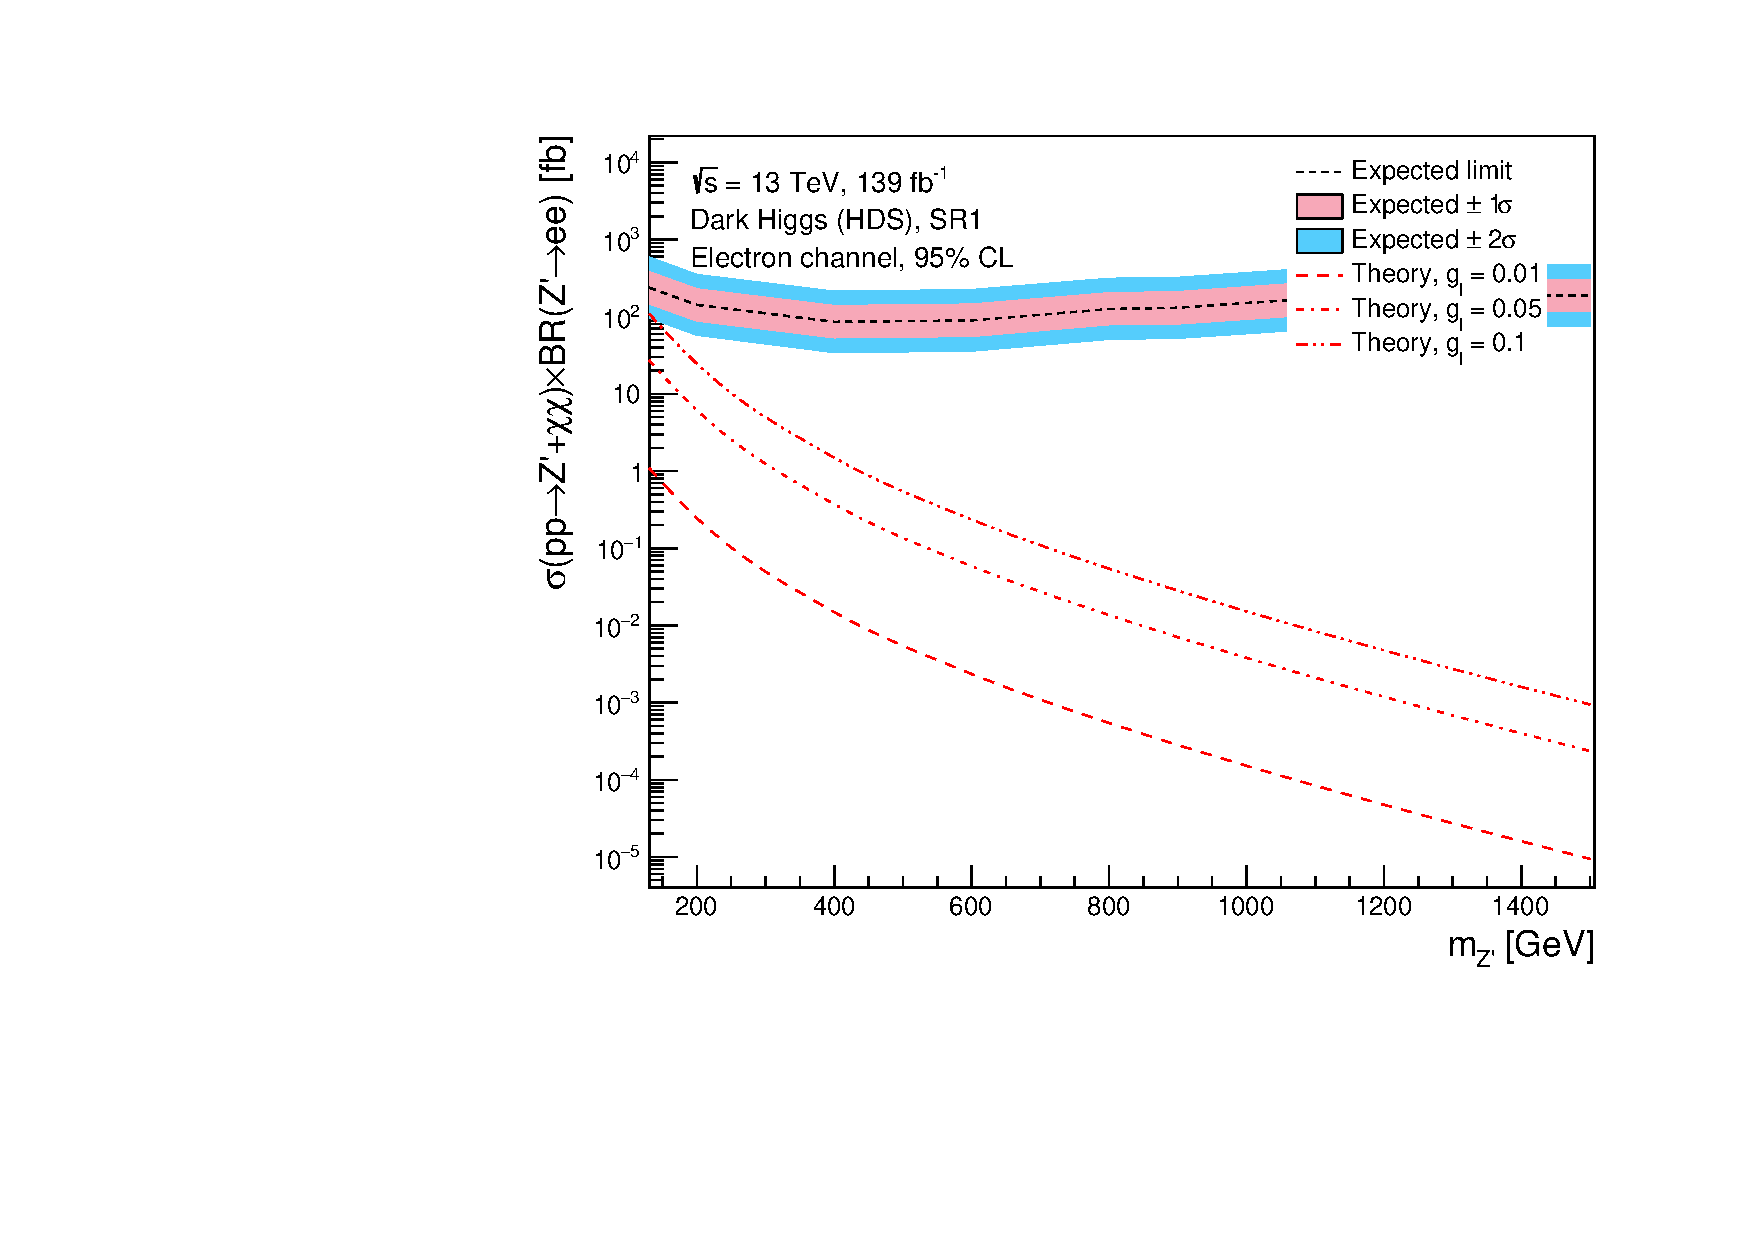
\includegraphics[width=1\textwidth]{Limits/Model_independent/50-100/DH_HDS/mass_exclusion_ee.pdf}
   \end{subfigure}
   \hfill
   \begin{subfigure}[b]{0.49\textwidth}
      \centering
      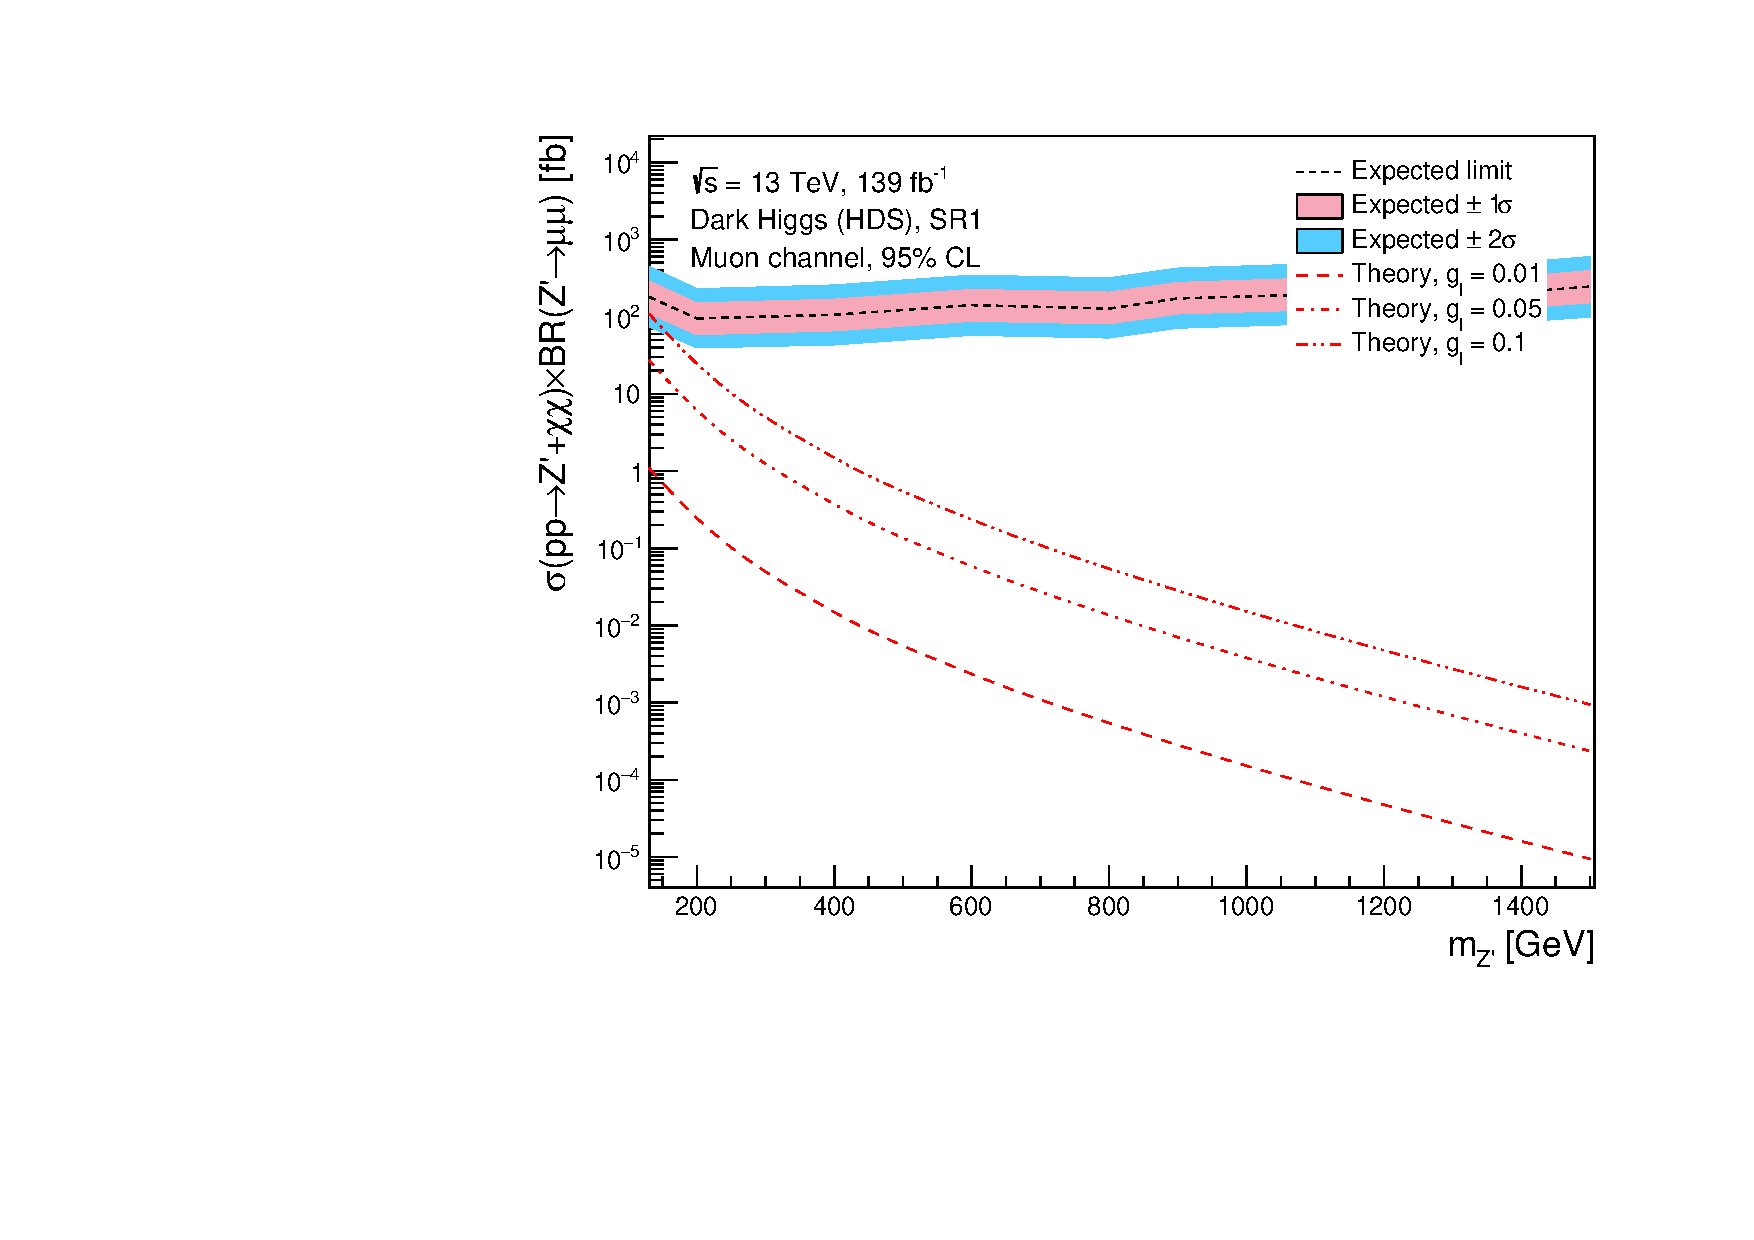
\includegraphics[width=1\textwidth]{Limits/Model_independent/50-100/DH_HDS/mass_exclusion_uu.pdf}
   \end{subfigure}
   \hfill
   \begin{subfigure}[b]{0.49\textwidth}
      \centering
      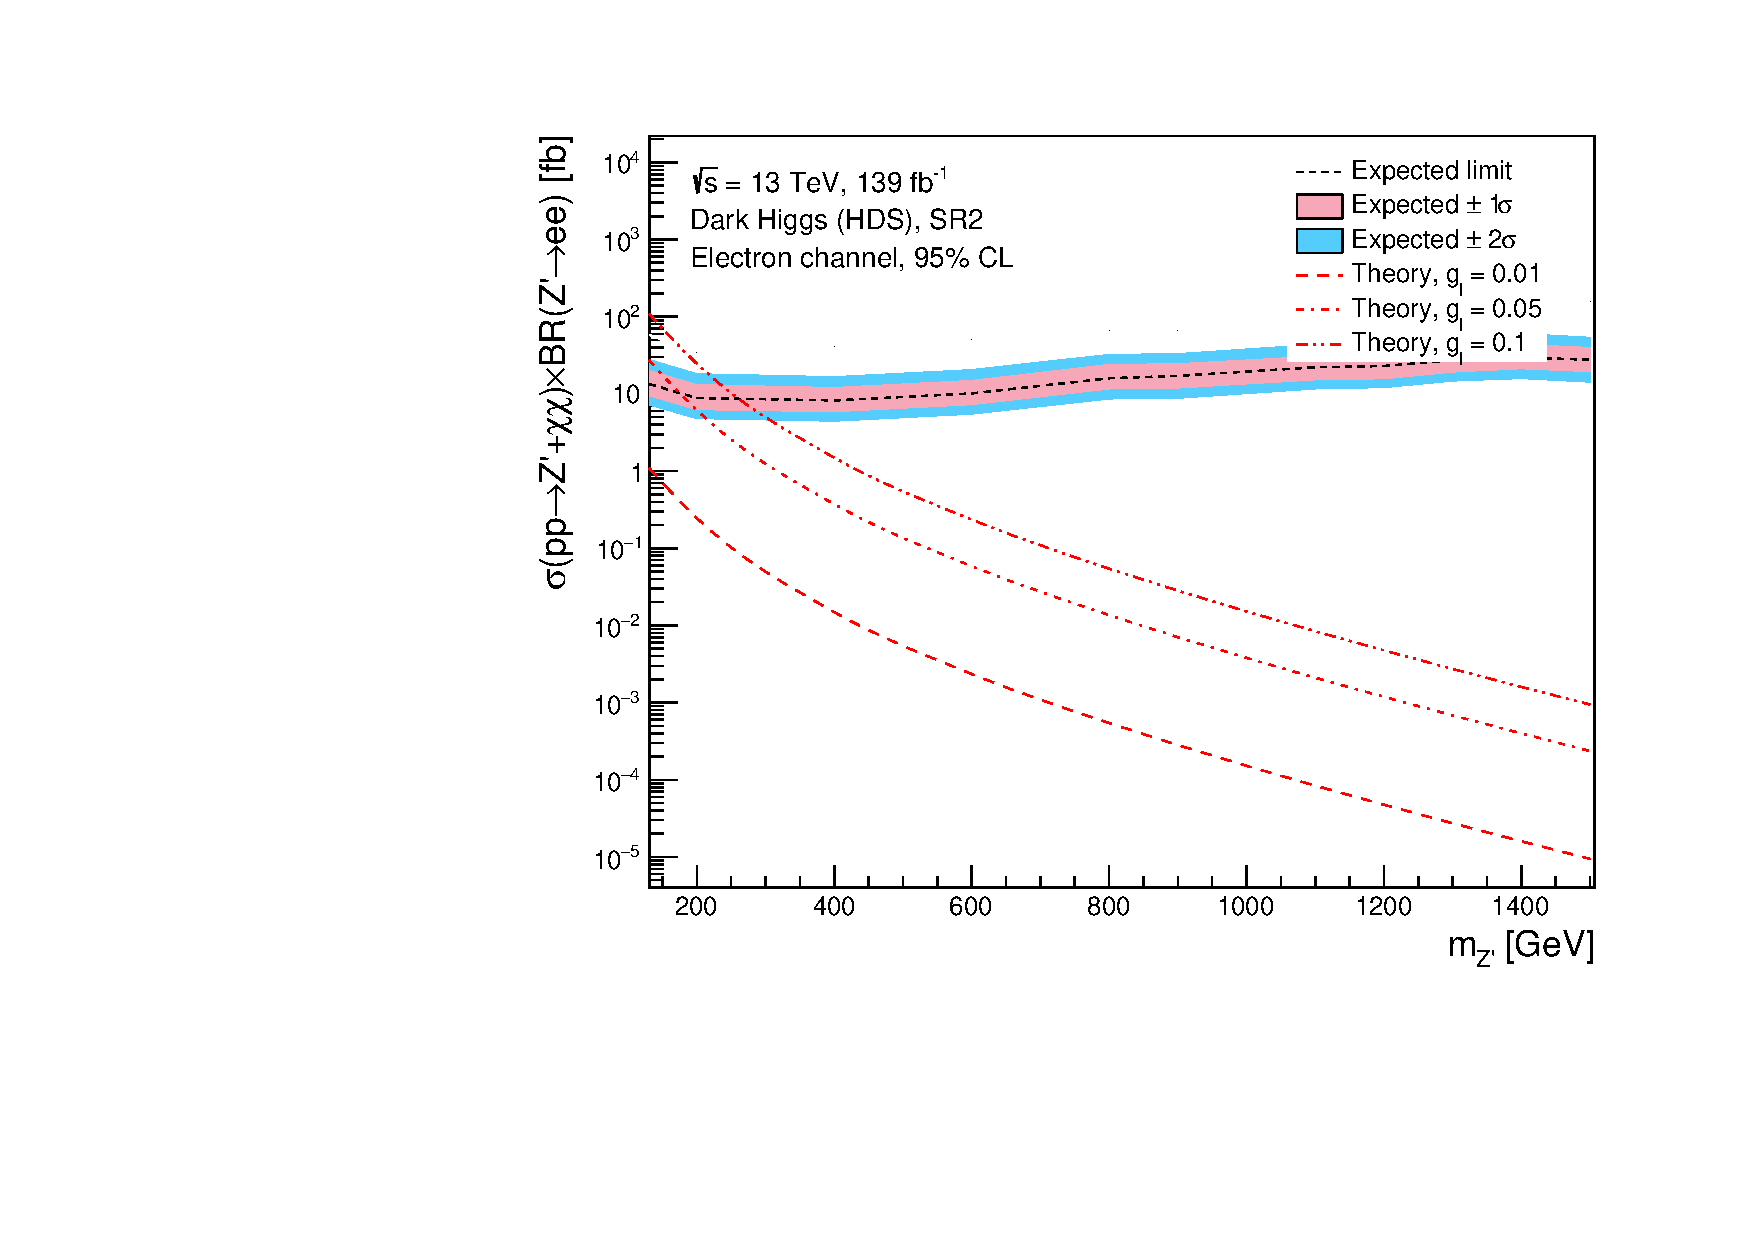
\includegraphics[width=1\textwidth]{Limits/Model_independent/100-150/DH_HDS/mass_exclusion_ee.pdf}
   \end{subfigure}
   \hfill
   \begin{subfigure}[b]{0.49\textwidth}
      \centering
      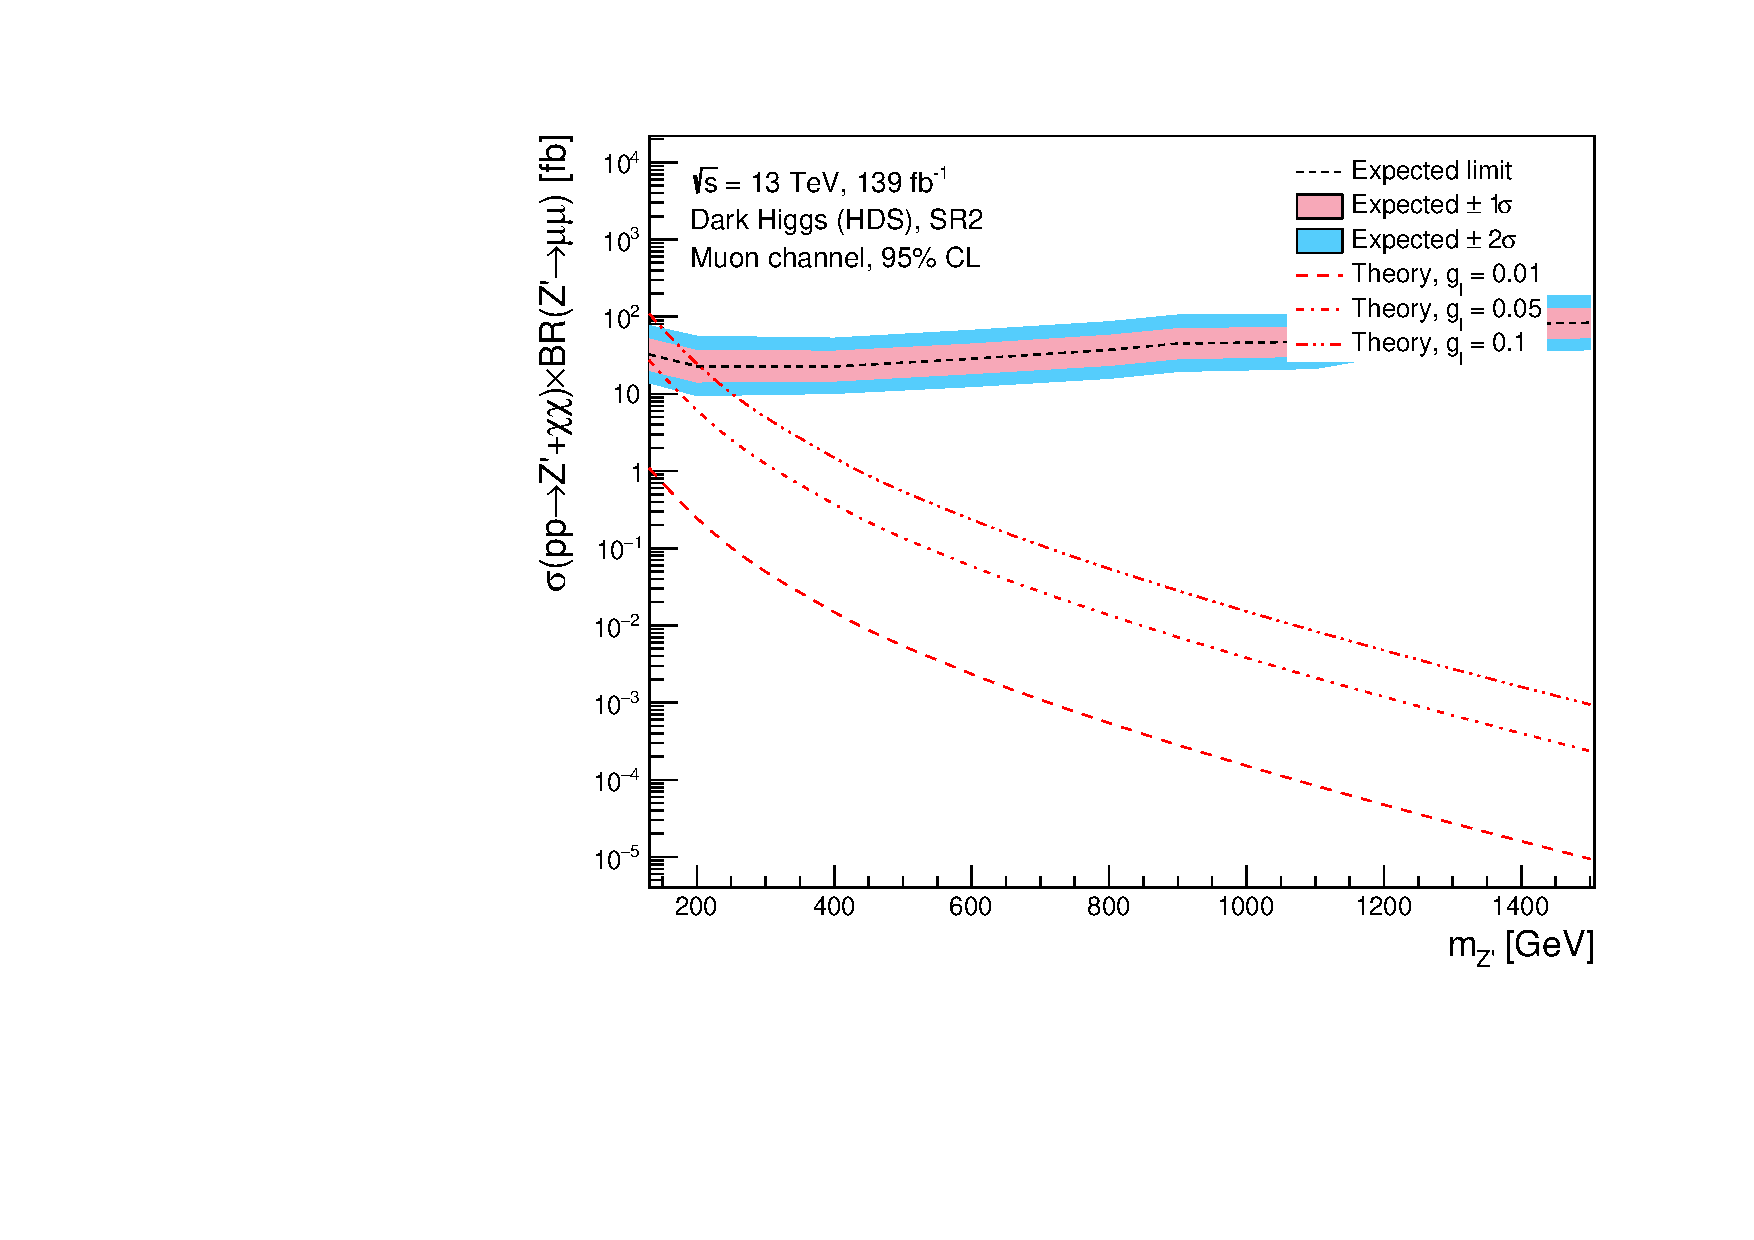
\includegraphics[width=1\textwidth]{Limits/Model_independent/100-150/DH_HDS/mass_exclusion_uu.pdf}
   \end{subfigure}
   \hfill
	\begin{subfigure}[b]{0.49\textwidth}
      \centering
      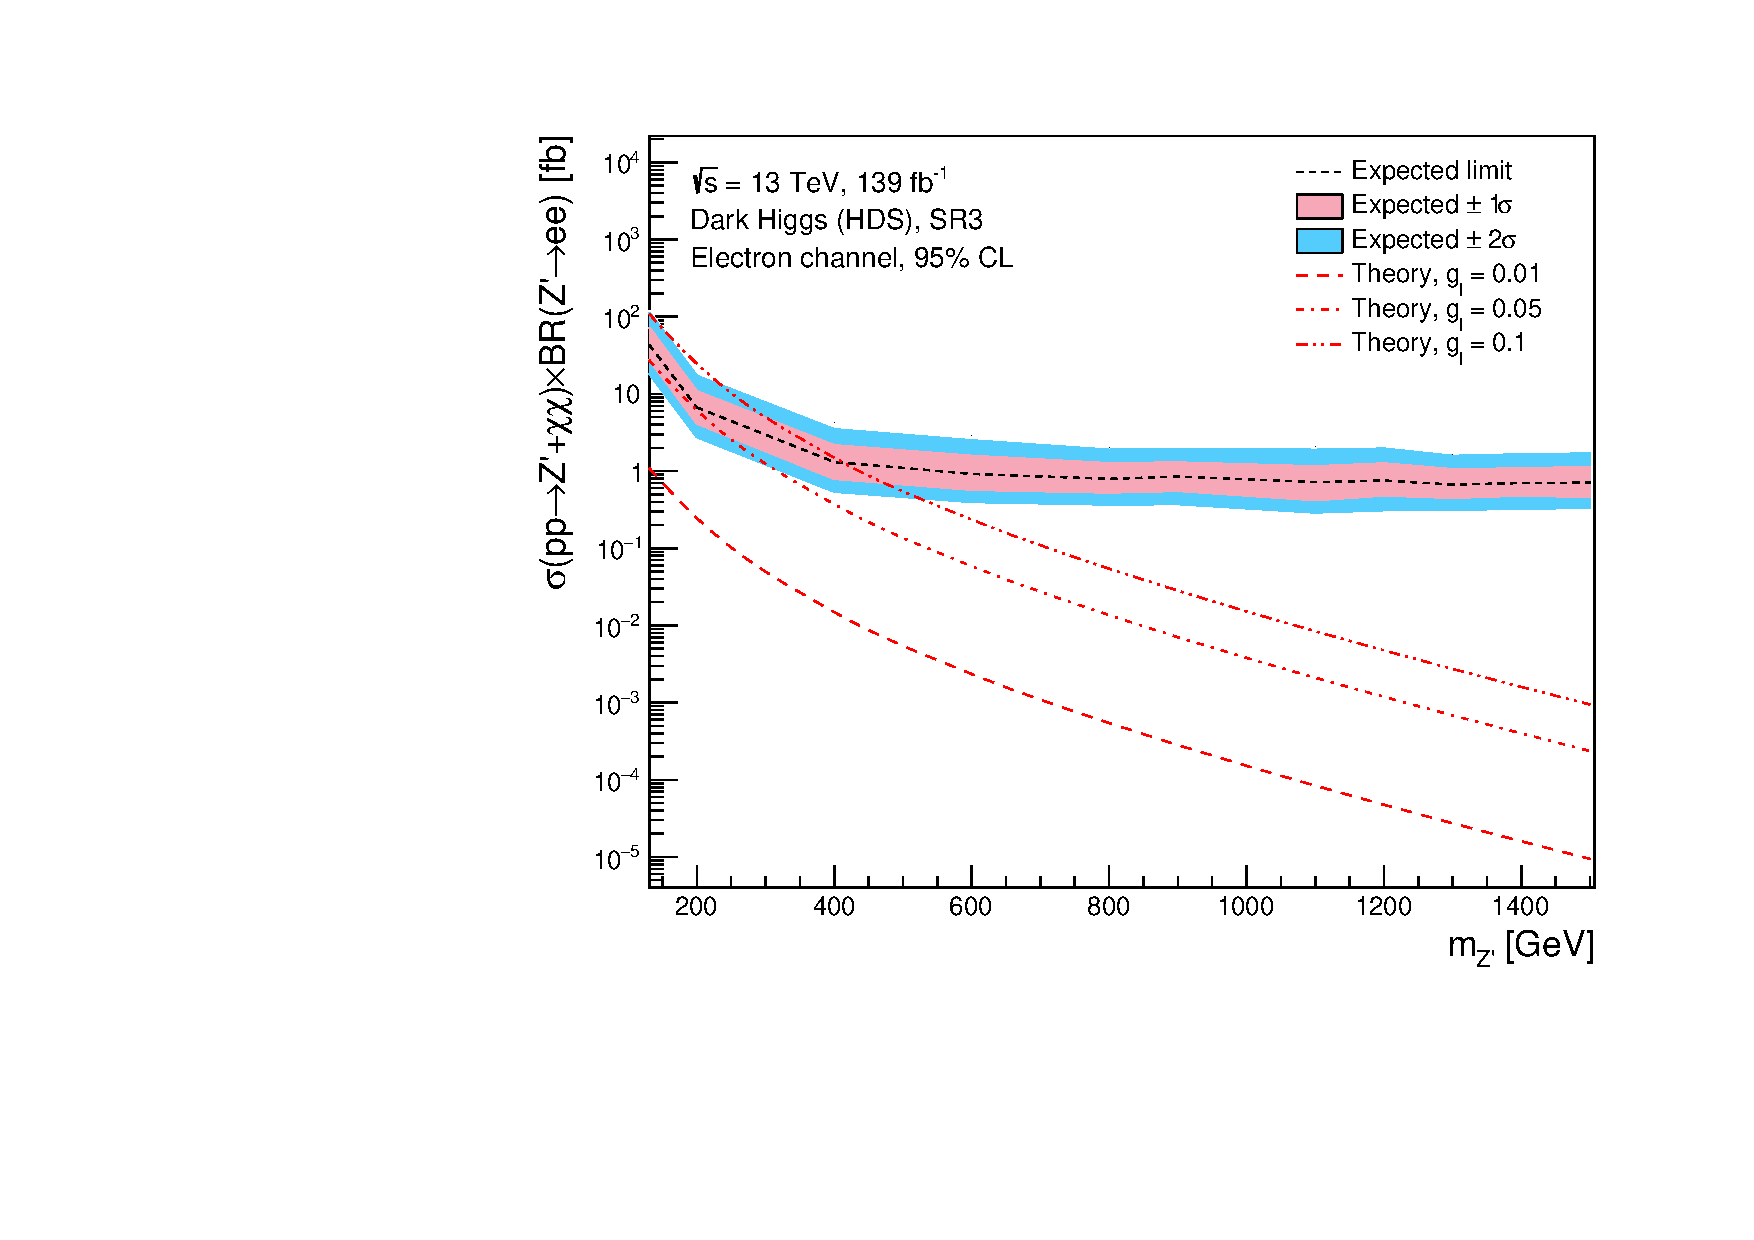
\includegraphics[width=1\textwidth]{Limits/Model_independent/150/DH_HDS/mass_exclusion_ee.pdf}
   \end{subfigure}
   \hfill
   \begin{subfigure}[b]{0.49\textwidth}
      \centering
      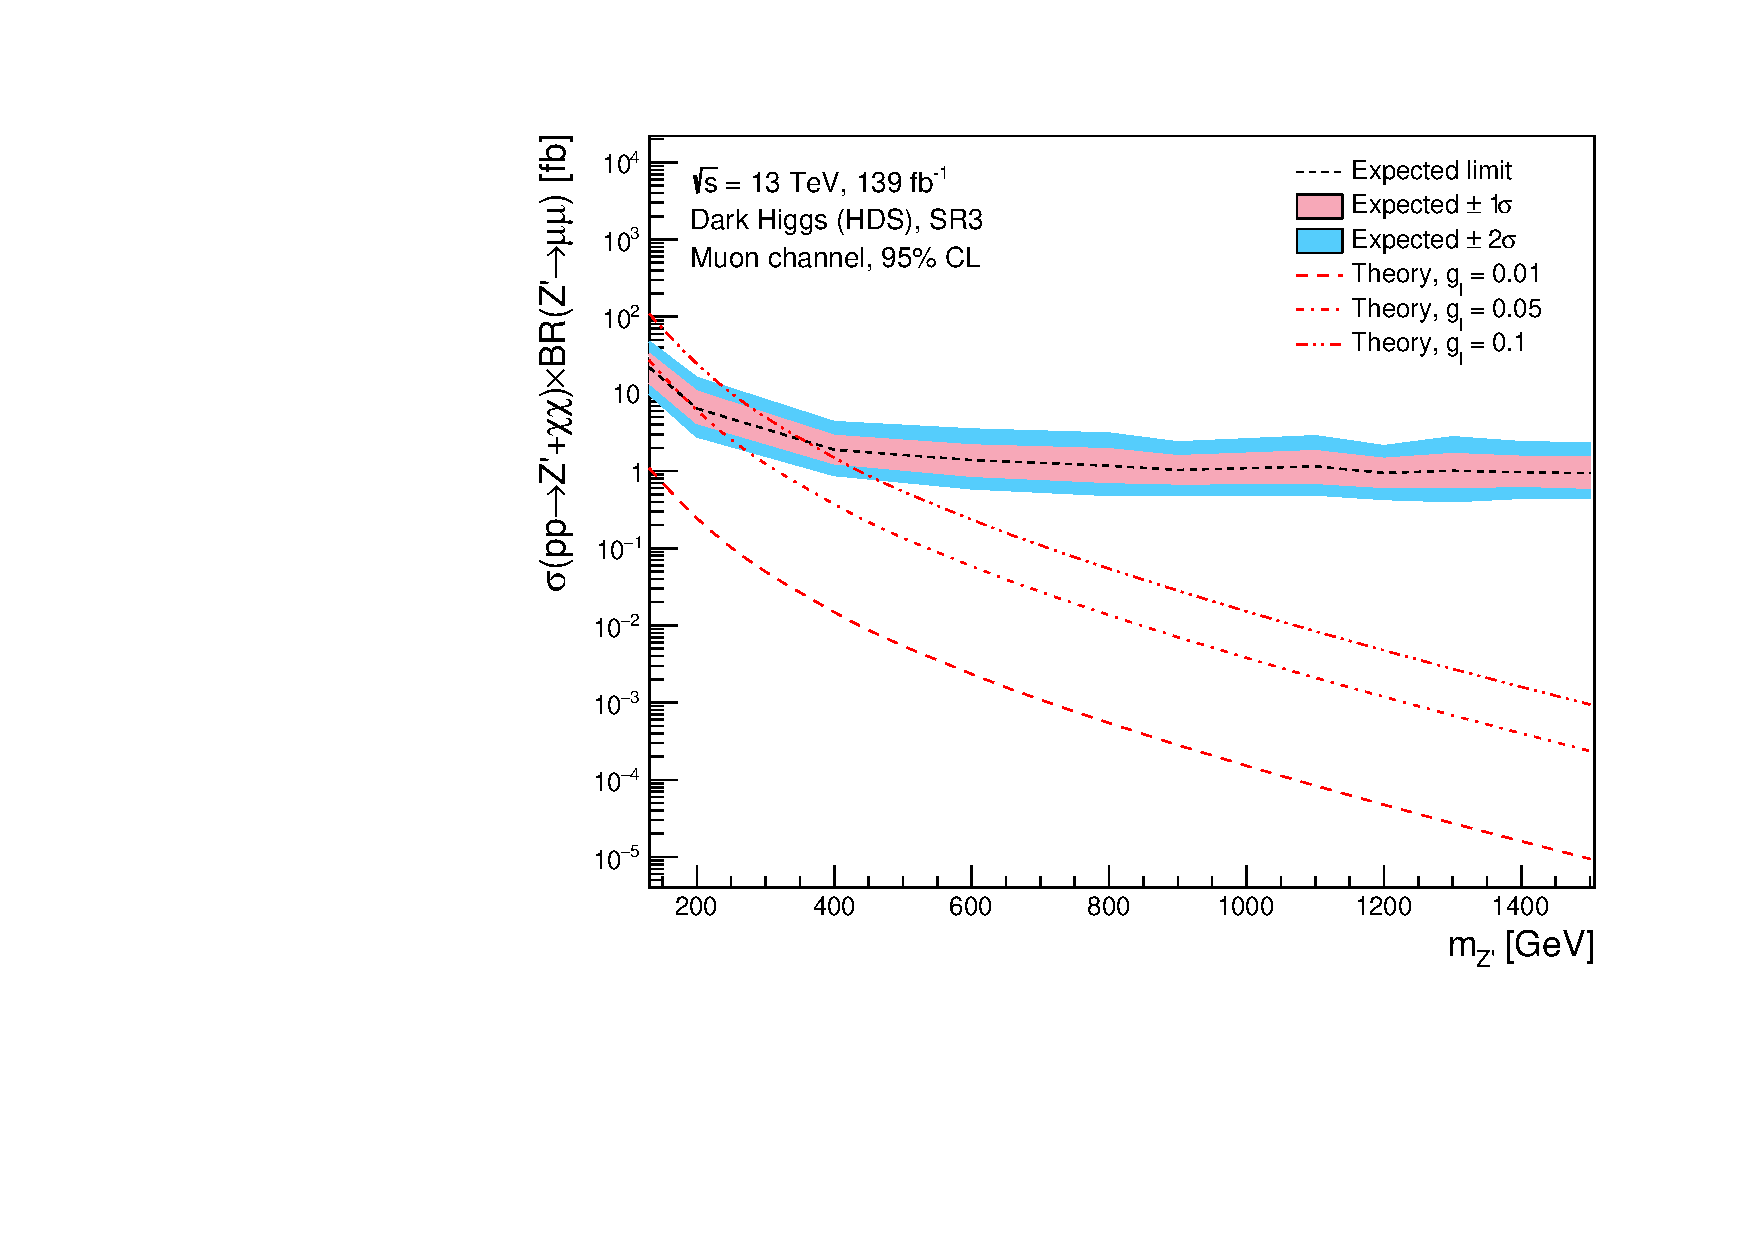
\includegraphics[width=1\textwidth]{Limits/Model_independent/150/DH_HDS/mass_exclusion_uu.pdf}
   \end{subfigure}
   \caption[Expected mass exclusion limits results for DH HDS model on $ee$ and $\mu\mu$ channel using the model independent approach]{Mass exclusion limits of $ee$ (left) and $\mu\mu$ (right) channel for Z' Dark Higgs Heavy Dark Sector model using the model independent approach. To remind what the SRs are: SR1 has $E_T^{miss}\in[50, 100]$ GeV, SR2 has $E_T^{miss}\in[100, 150]$ GeV, and SR3 has $E_T^{miss}>150$ GeV. The y-axis of both plots represents the cross-section times branching ratio of the process we are studying. The x-axis is the mass of the $Z'$ boson. We did not interpolate between the available masses we had simulated, 
   and have rather just connected the values calculated for each mass point by connecting the points. The dashed black line is the expected 95\% CL limit with a 1$\sigma$ and 2$\sigma$ variance. 
   The different red dashed lines represent the theoretical cross-section times branching ratio of the process when varying the value of the lepton coupling $g_l$ between the leptons and the $Z'$ boson. The simulated events in this thesis utilized the value $g_l=$ 0.01, we include the cross-section times branching ratio when increasing this coupling to 0.05 and 0.1 to see how the exclusions change.  }
\end{figure}


\clearpage
\section{Dark Higgs Light Dark Sector}
\begin{figure}[!ht]
	\centering
   \begin{subfigure}[b]{0.49\textwidth}
      \centering
      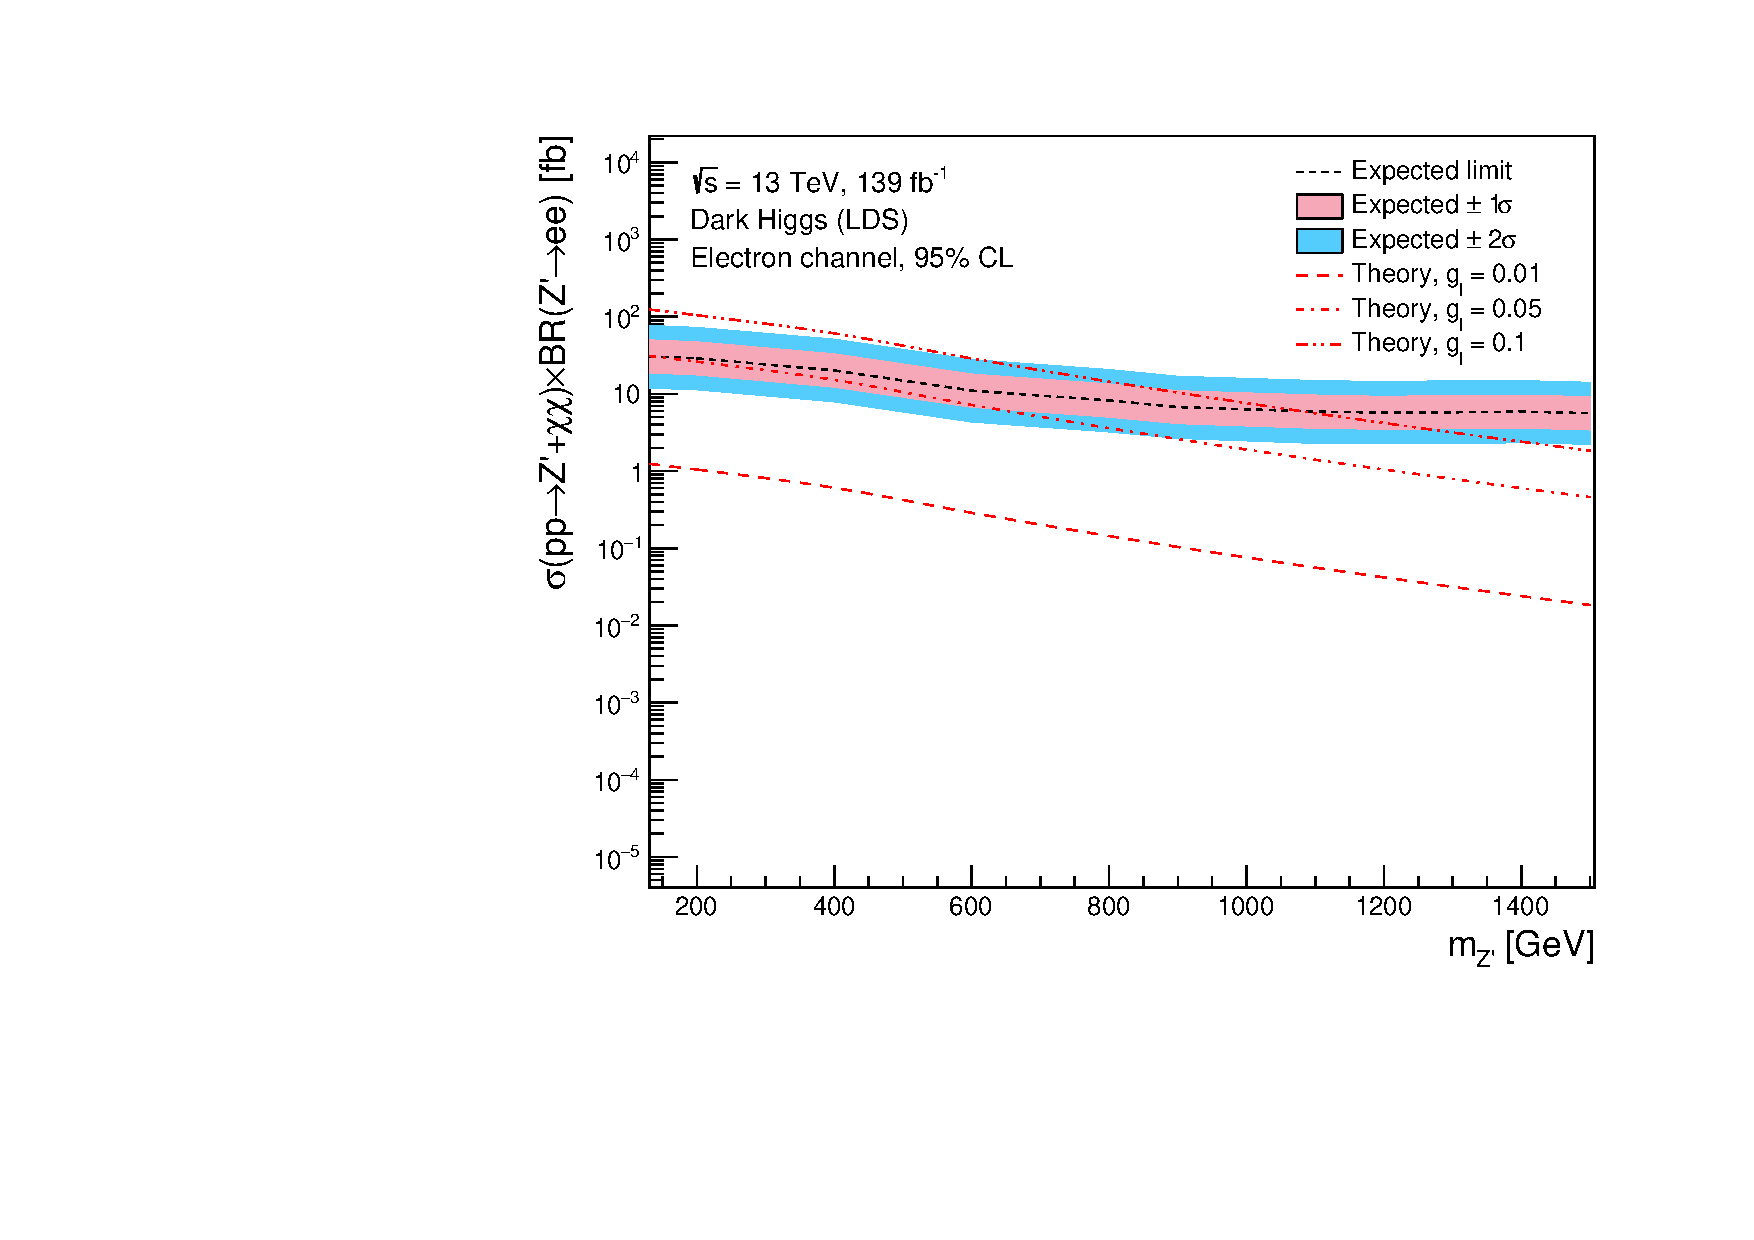
\includegraphics[width=1\textwidth]{Limits/DH_LDS/mass_exclusion_ee.pdf}
      \end{subfigure}
   \hfill
   \begin{subfigure}[b]{0.49\textwidth}
      \centering
      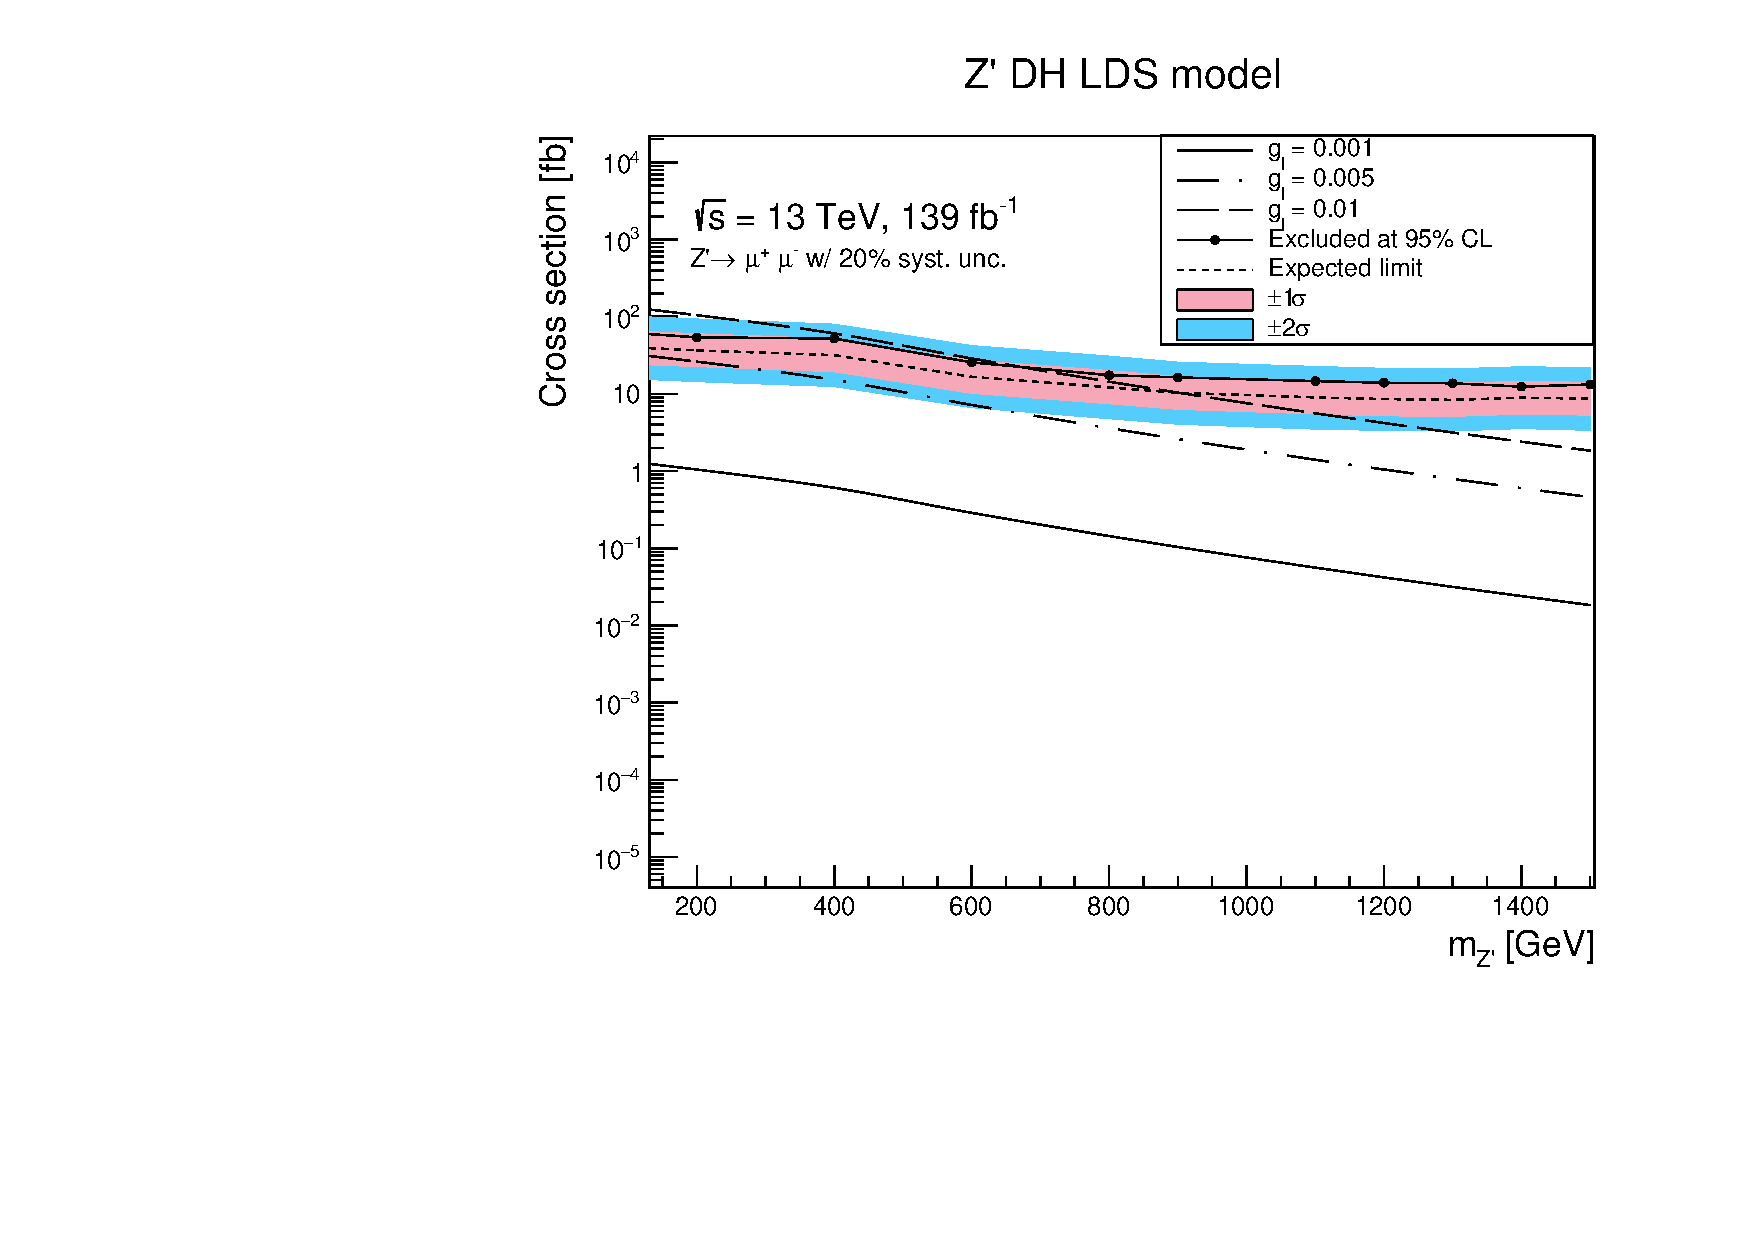
\includegraphics[width=1\textwidth]{Limits/DH_LDS/mass_exclusion_uu.pdf}
      \end{subfigure}
   \caption[Expected mass exclusion limits of $ee$ and $\mu\mu$ channel for all Z' DH LDS model using the model dependent approach]{Mass exclusion limits of $ee$ (left) and $\mu\mu$ (right) channel for Z' Dark Higgs Light Dark Sector model using the model dependent approach. The y-axis of both plots represents the cross-section times branching ratio of the process we are studying. The x-axis is the mass of the $Z'$ boson. We did not interpolate between the available masses we had simulated, 
   and have rather just connected the values calculated for each mass point by connecting the points. The dashed black line is the expected 95\% CL limit with a 1$\sigma$ and 2$\sigma$ variance. 
   The different red dashed lines represent the theoretical cross-section times branching ratio of the process when varying the value of the lepton coupling $g_l$ between the leptons and the $Z'$ boson. The simulated events in this thesis utilized the value $g_l=$ 0.01, we include the cross-section times branching ratio when increasing this coupling to 0.05 and 0.1 to see how the exclusions change.  }\label{fig:DH_LDS_exclusion_ee_uu}
\end{figure}

\begin{figure}[!ht]
	\centering
	\begin{subfigure}[b]{0.49\textwidth}
      \centering
      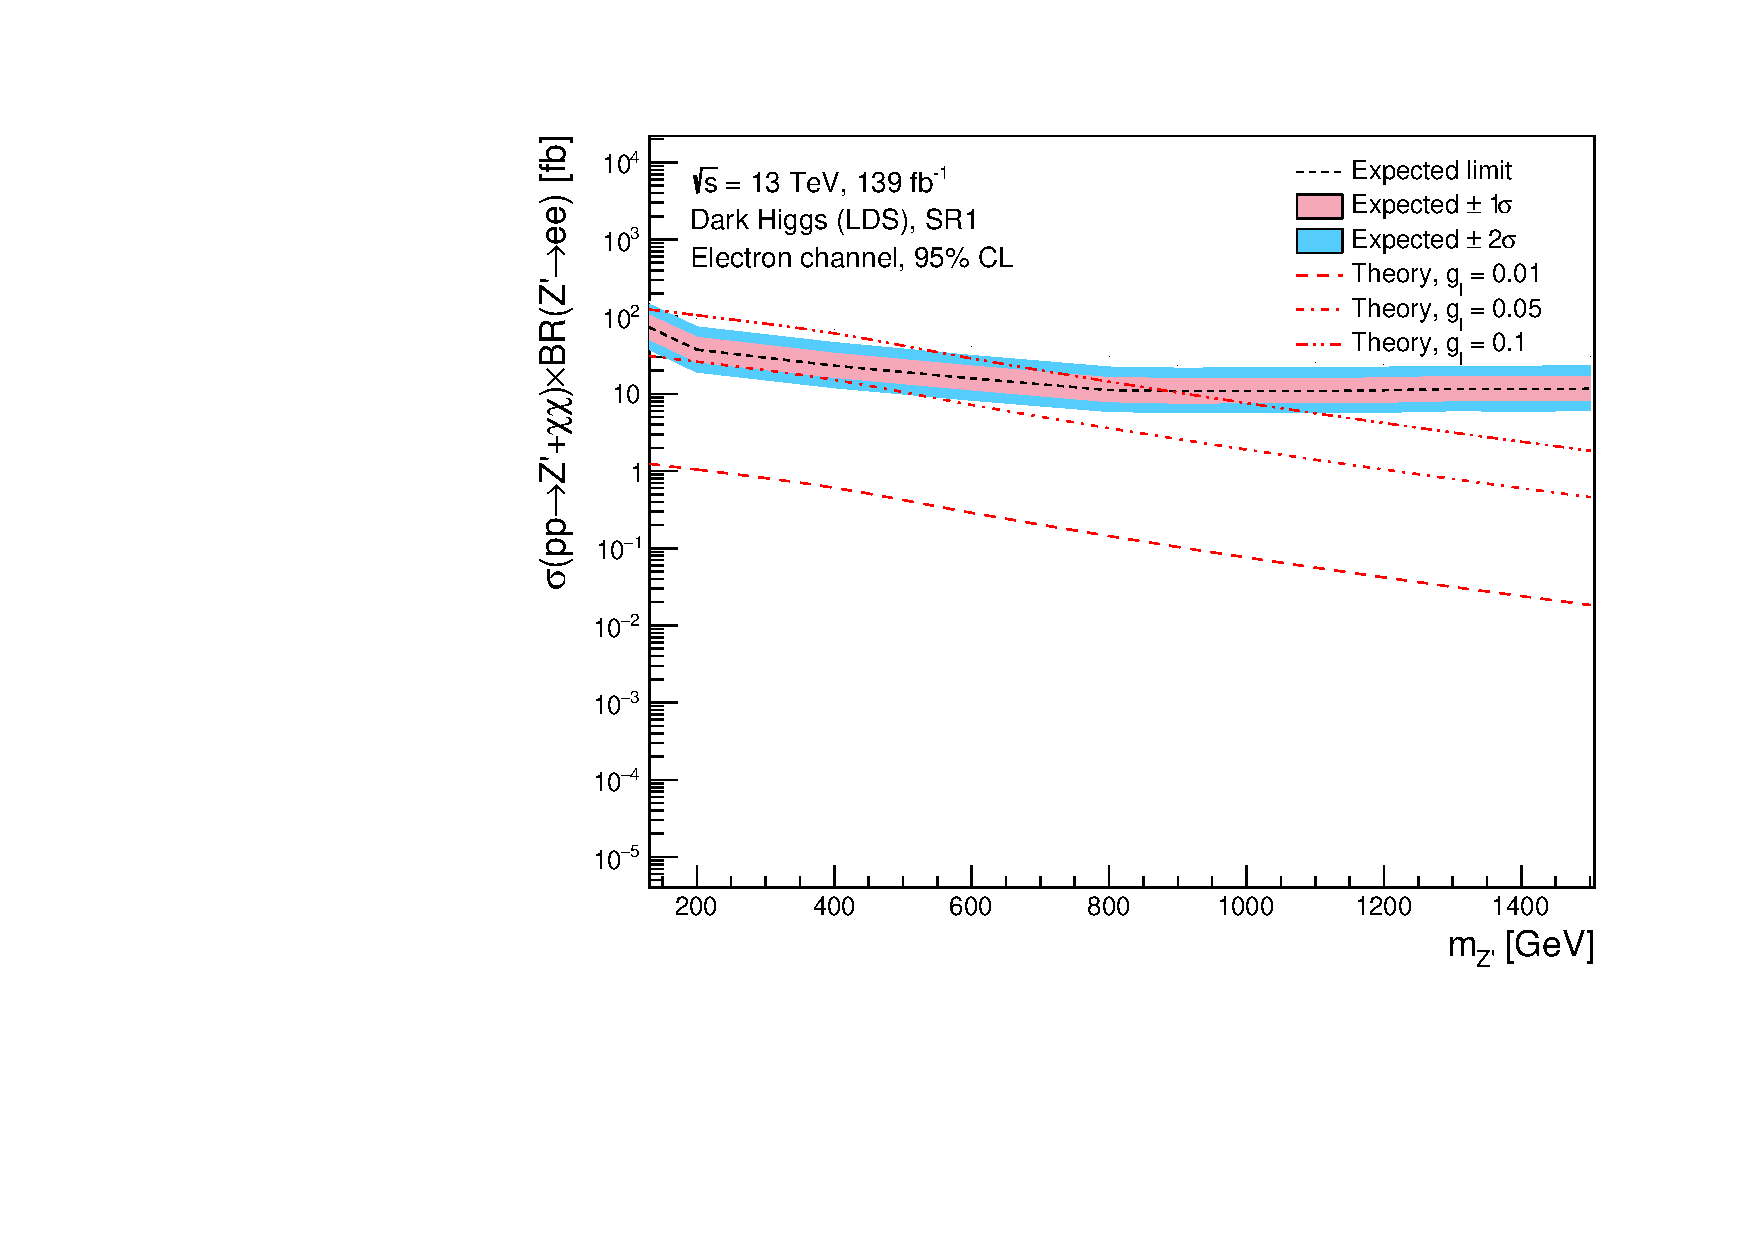
\includegraphics[width=1\textwidth]{Limits/Model_independent/50-100/DH_LDS/mass_exclusion_ee.pdf}
   \end{subfigure}
   \hfill
   \begin{subfigure}[b]{0.49\textwidth}
      \centering
      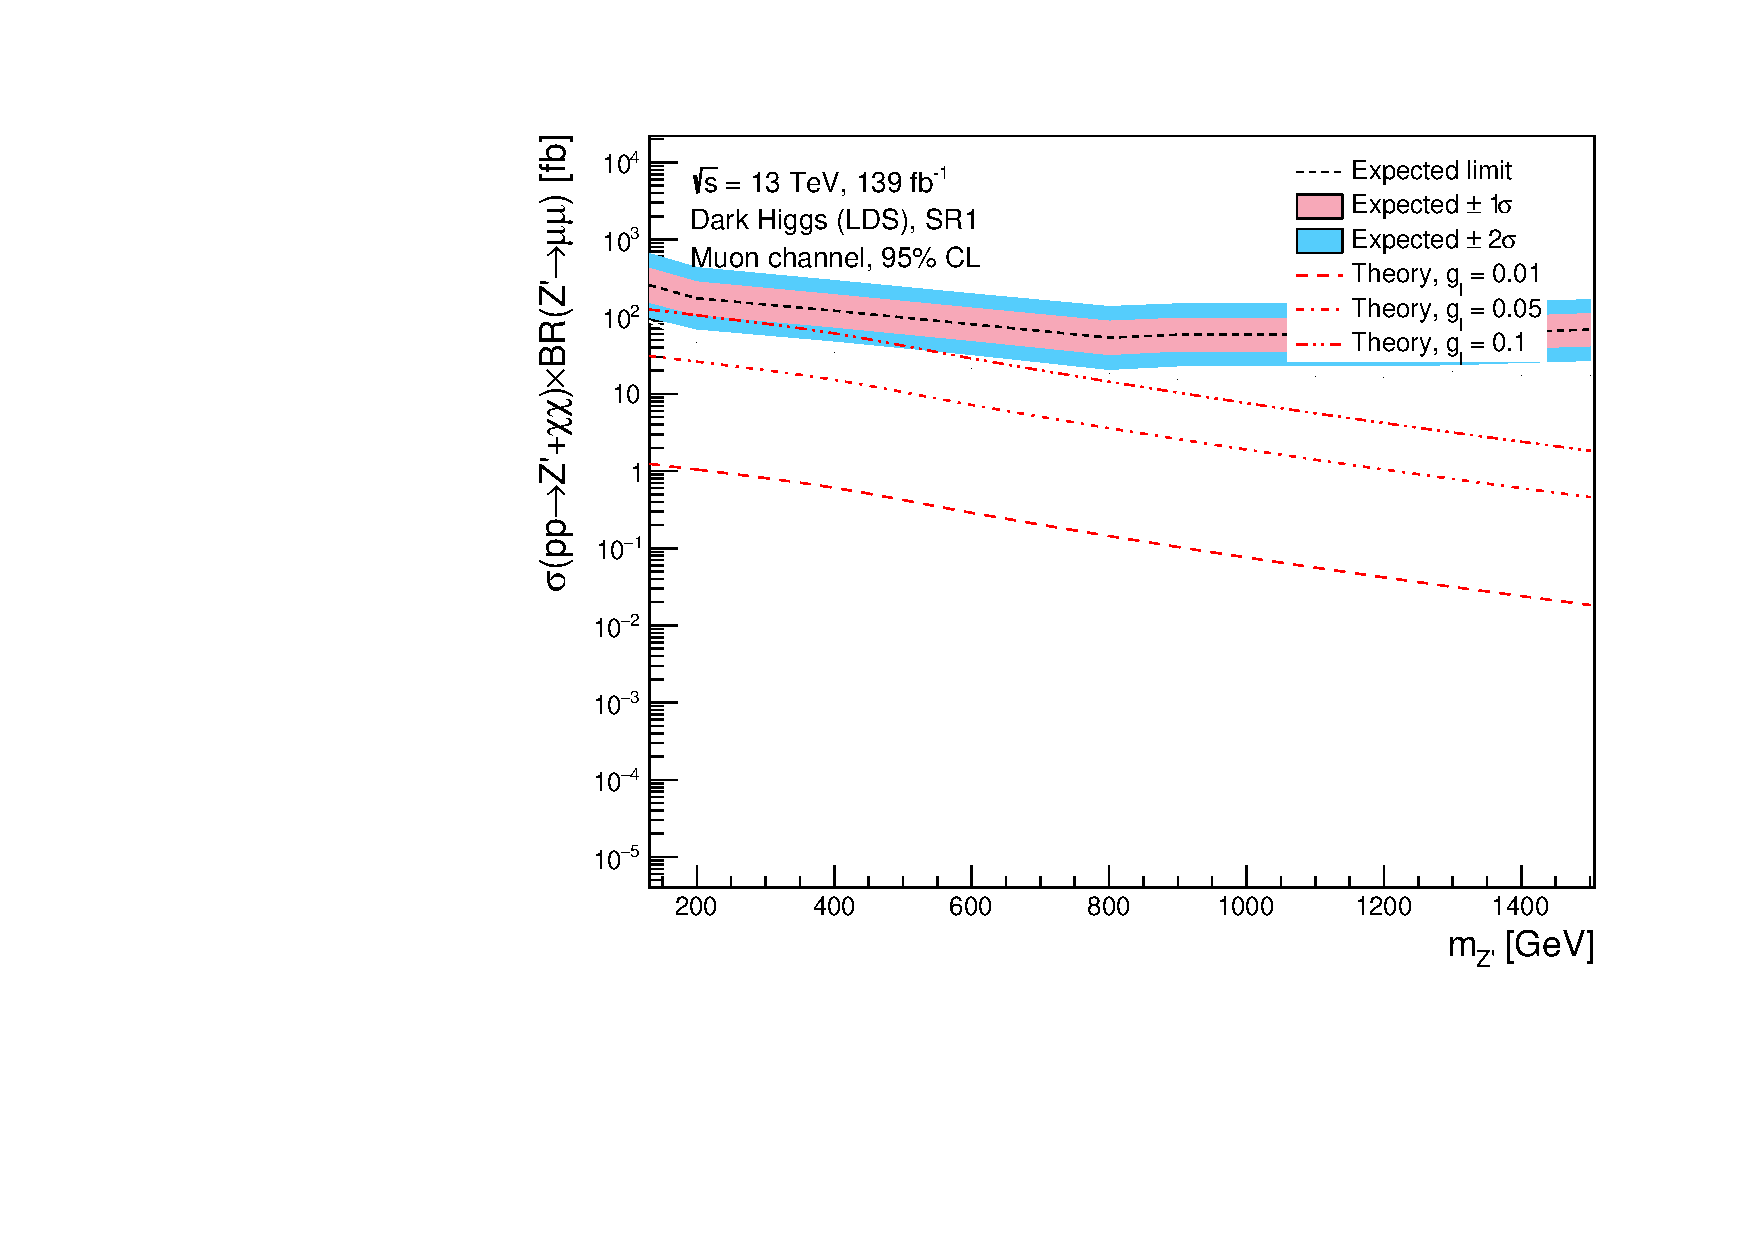
\includegraphics[width=1\textwidth]{Limits/Model_independent/50-100/DH_LDS/mass_exclusion_uu.pdf}
   \end{subfigure}
   \hfill
   \begin{subfigure}[b]{0.49\textwidth}
      \centering
      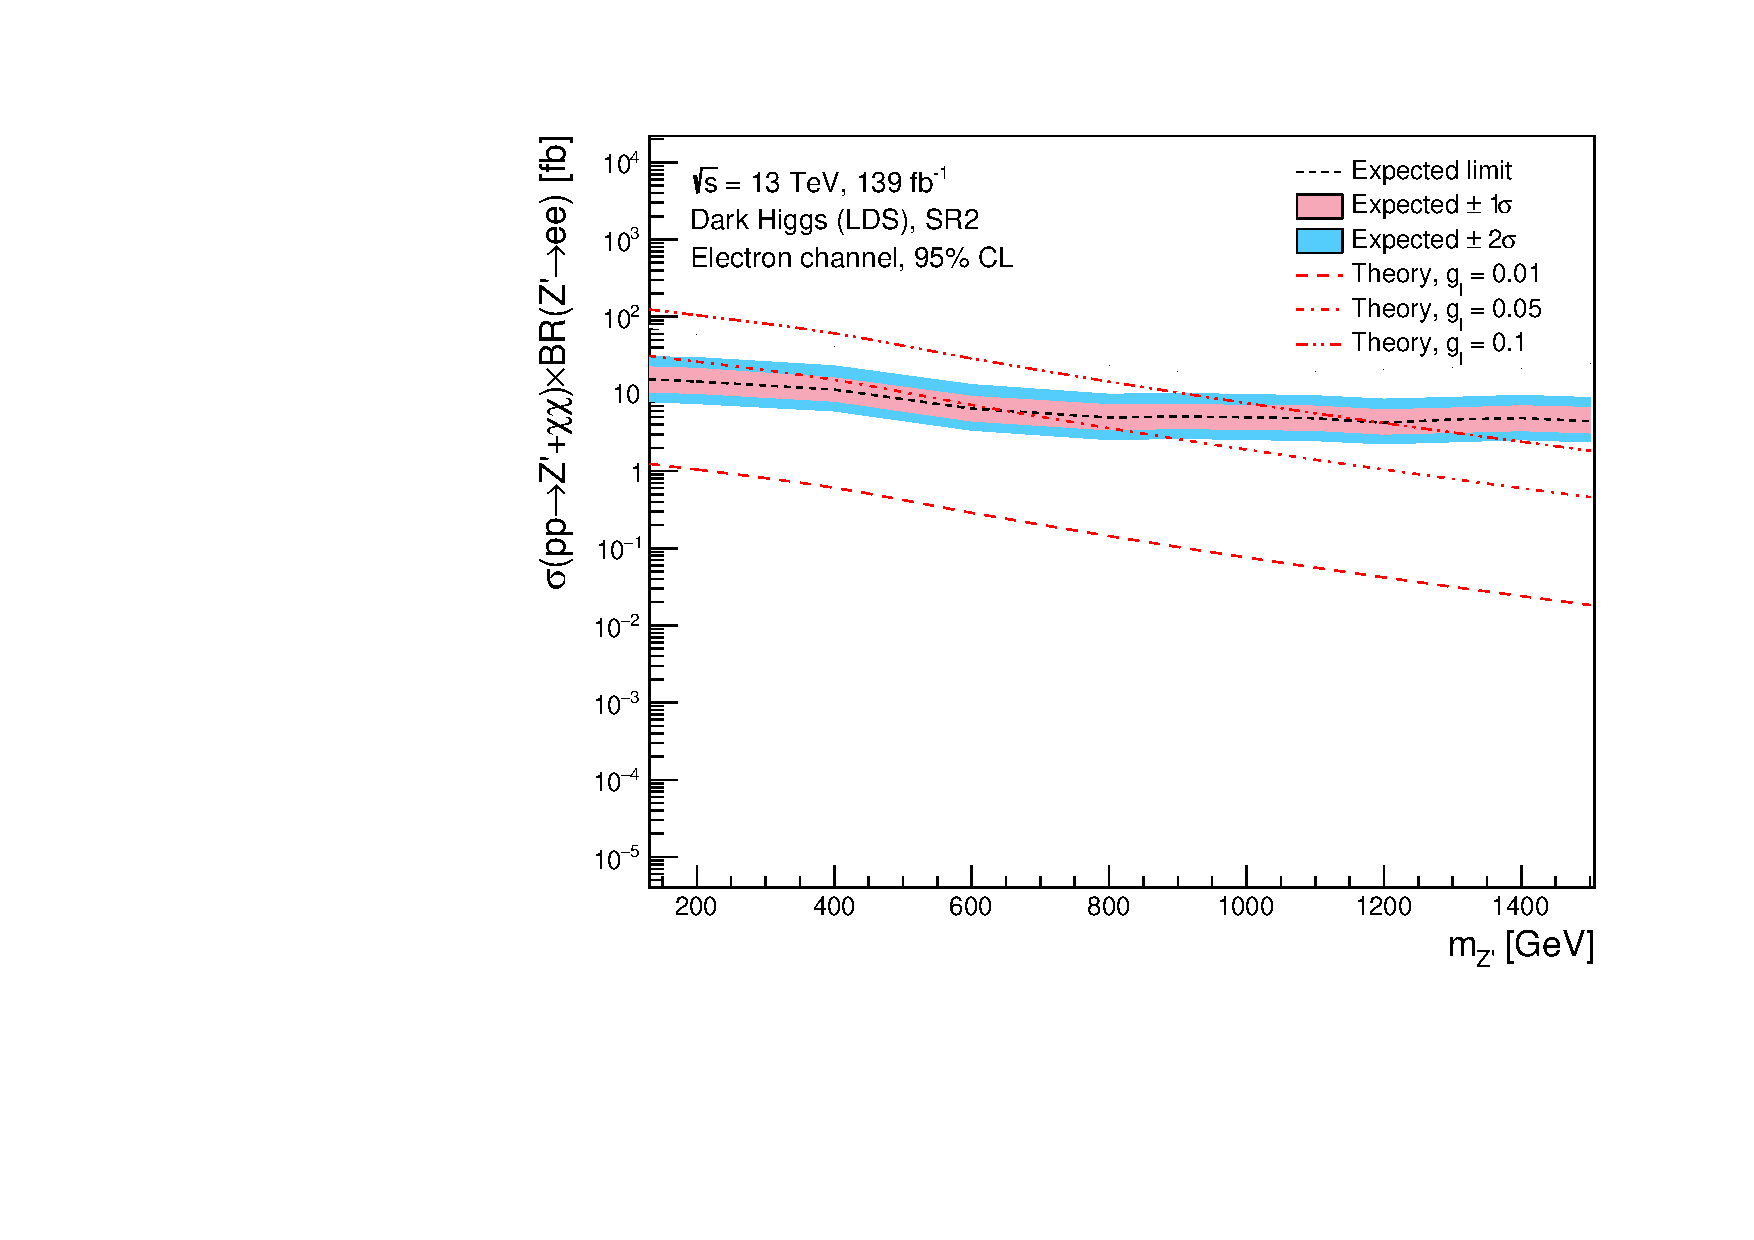
\includegraphics[width=1\textwidth]{Limits/Model_independent/100-150/DH_LDS/mass_exclusion_ee.pdf}
   \end{subfigure}
   \hfill
   \begin{subfigure}[b]{0.49\textwidth}
      \centering
      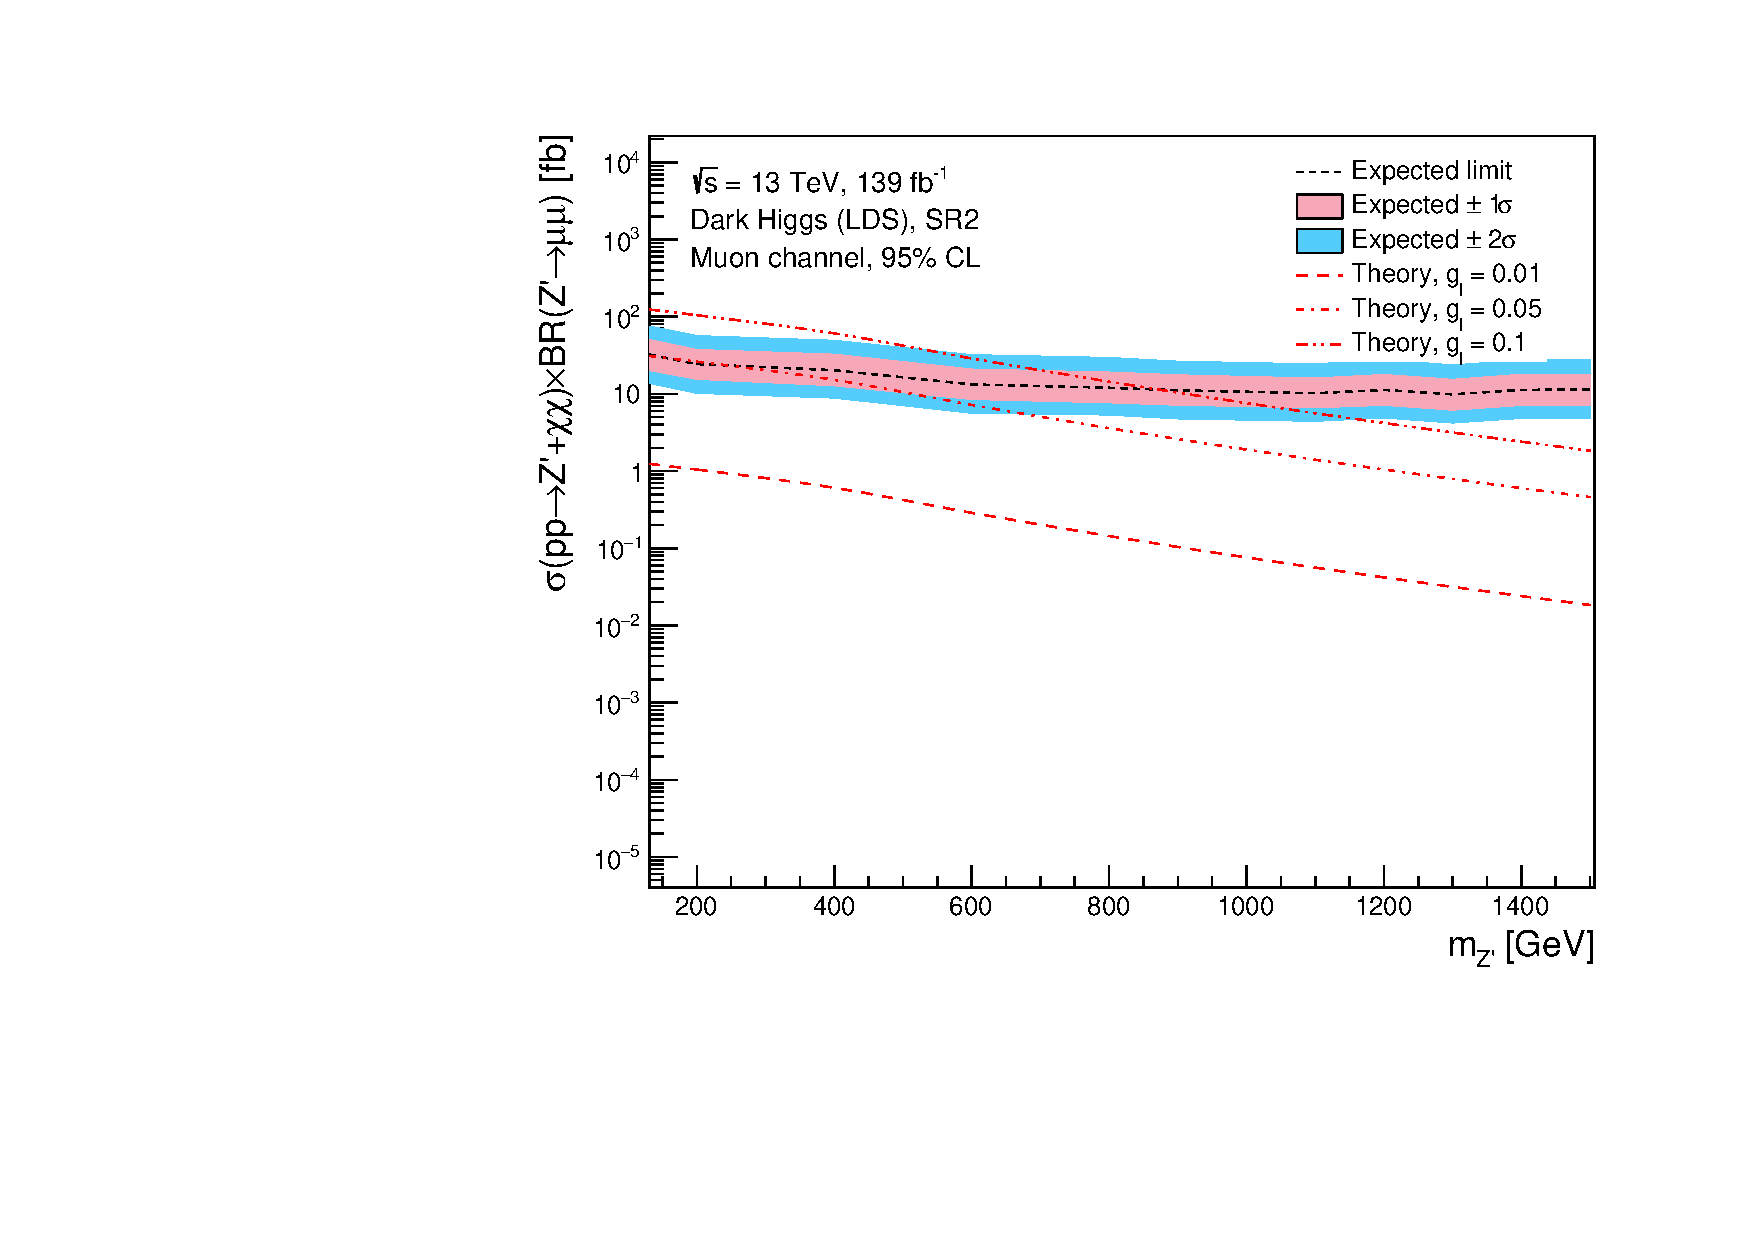
\includegraphics[width=1\textwidth]{Limits/Model_independent/100-150/DH_LDS/mass_exclusion_uu.pdf}
   \end{subfigure}
   \hfill
	\begin{subfigure}[b]{0.49\textwidth}
      \centering
      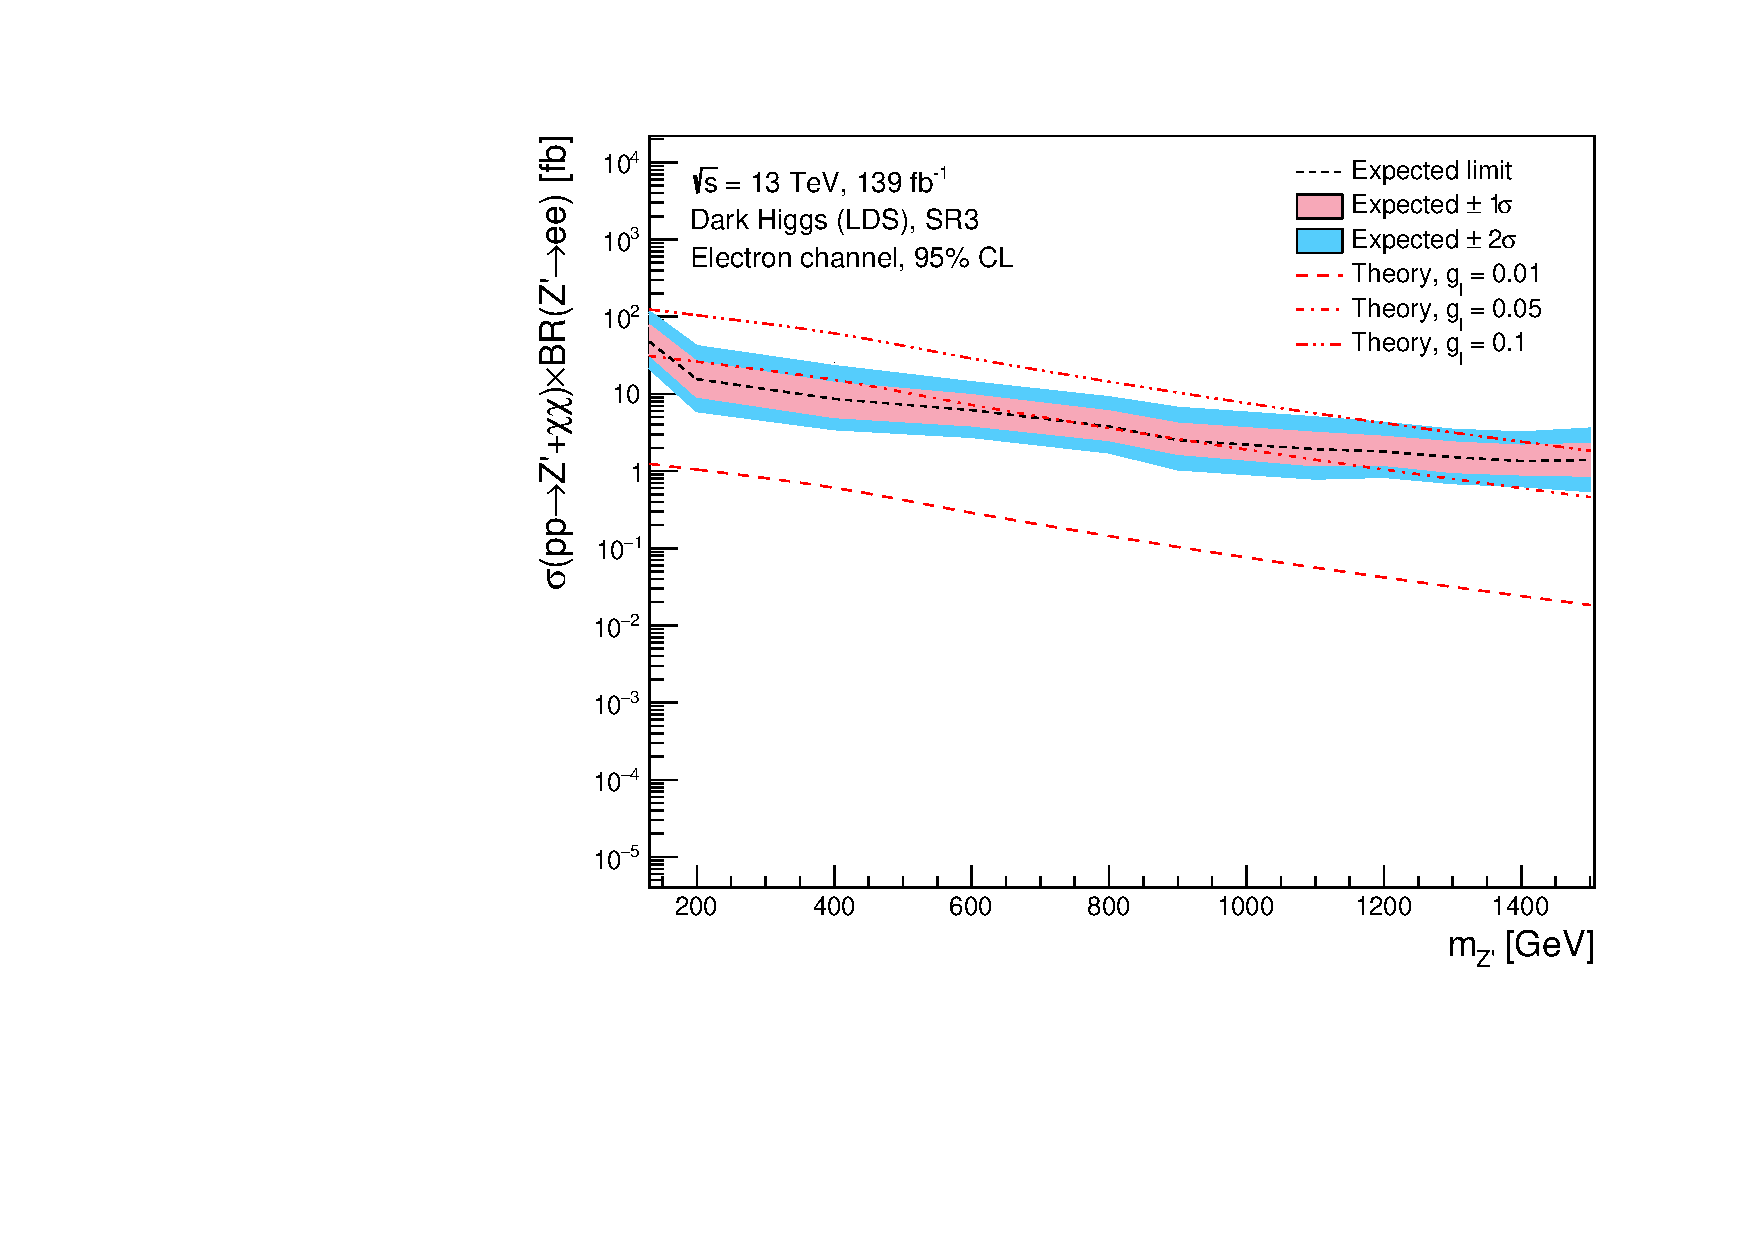
\includegraphics[width=1\textwidth]{Limits/Model_independent/150/DH_LDS/mass_exclusion_ee.pdf}
   \end{subfigure}
   \hfill
   \begin{subfigure}[b]{0.49\textwidth}
      \centering
      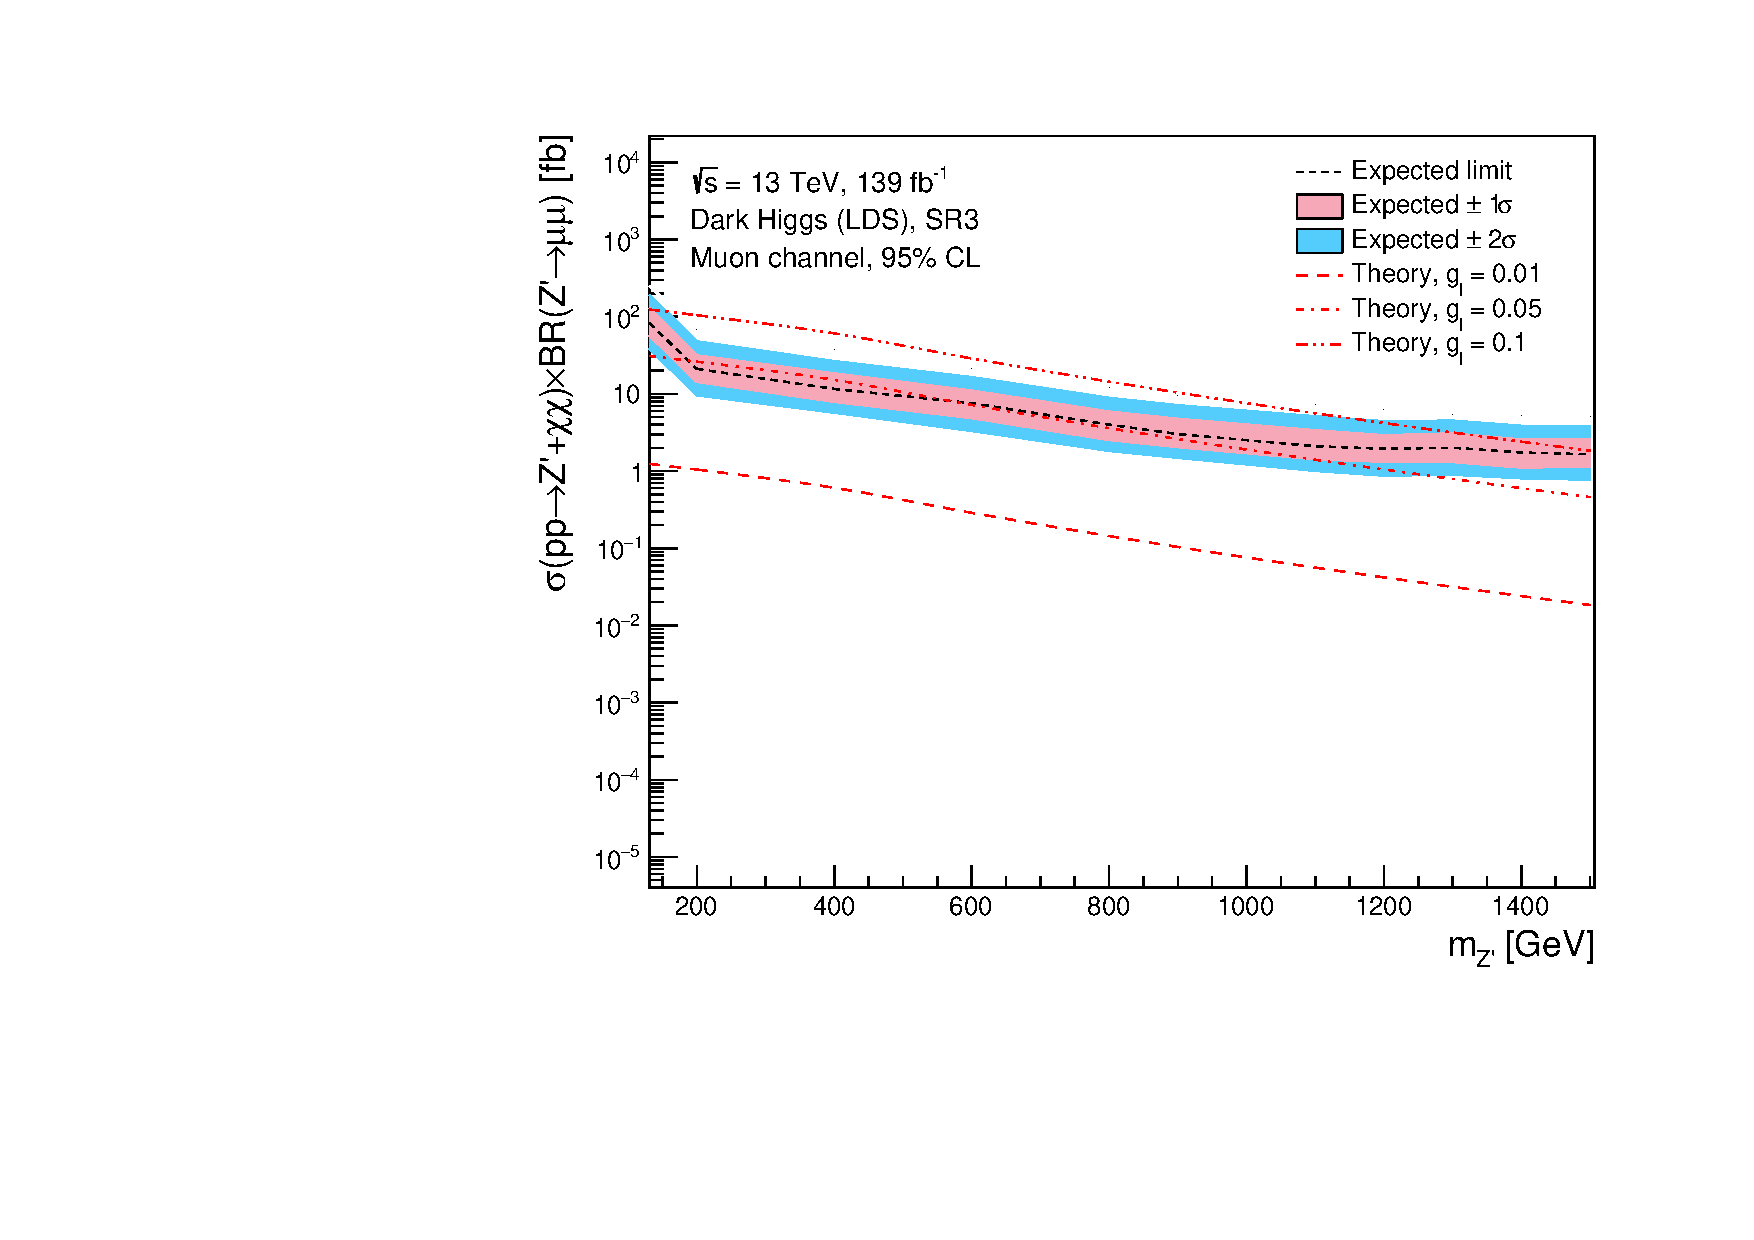
\includegraphics[width=1\textwidth]{Limits/Model_independent/150/DH_LDS/mass_exclusion_uu.pdf}
   \end{subfigure}
   \caption[Expected mass exclusion limits results for DH LDS model on $ee$ and $\mu\mu$ channel using the model independent approach]{Mass exclusion limits of $ee$ (left) and $\mu\mu$ (right) channel for Z' Dark Higgs Light Dark Sector model using the model independent approach. The y-axis of both plots represents the cross-section times branching ratio of the process we are studying. The x-axis is the mass of the $Z'$ boson. We did not interpolate between the available masses we had simulated, 
   and have rather just connected the values calculated for each mass point by connecting the points. The dashed black line is the expected 95\% CL limit with a 1$\sigma$ and 2$\sigma$ variance. 
   The different red dashed lines represent the theoretical cross-section times branching ratio of the process when varying the value of the lepton coupling $g_l$ between the leptons and the $Z'$ boson. The simulated events in this thesis utilized the value $g_l=$ 0.01, we include the cross-section times branching ratio when increasing this coupling to 0.05 and 0.1 to see how the exclusions change.  }\label{fig:DH_LDS_me_SRS}
\end{figure}





\clearpage
\section{Light Vector Heavy Dark Sector}
\begin{figure}[!ht]
	\centering
   \begin{subfigure}[b]{0.49\textwidth}
      \centering
      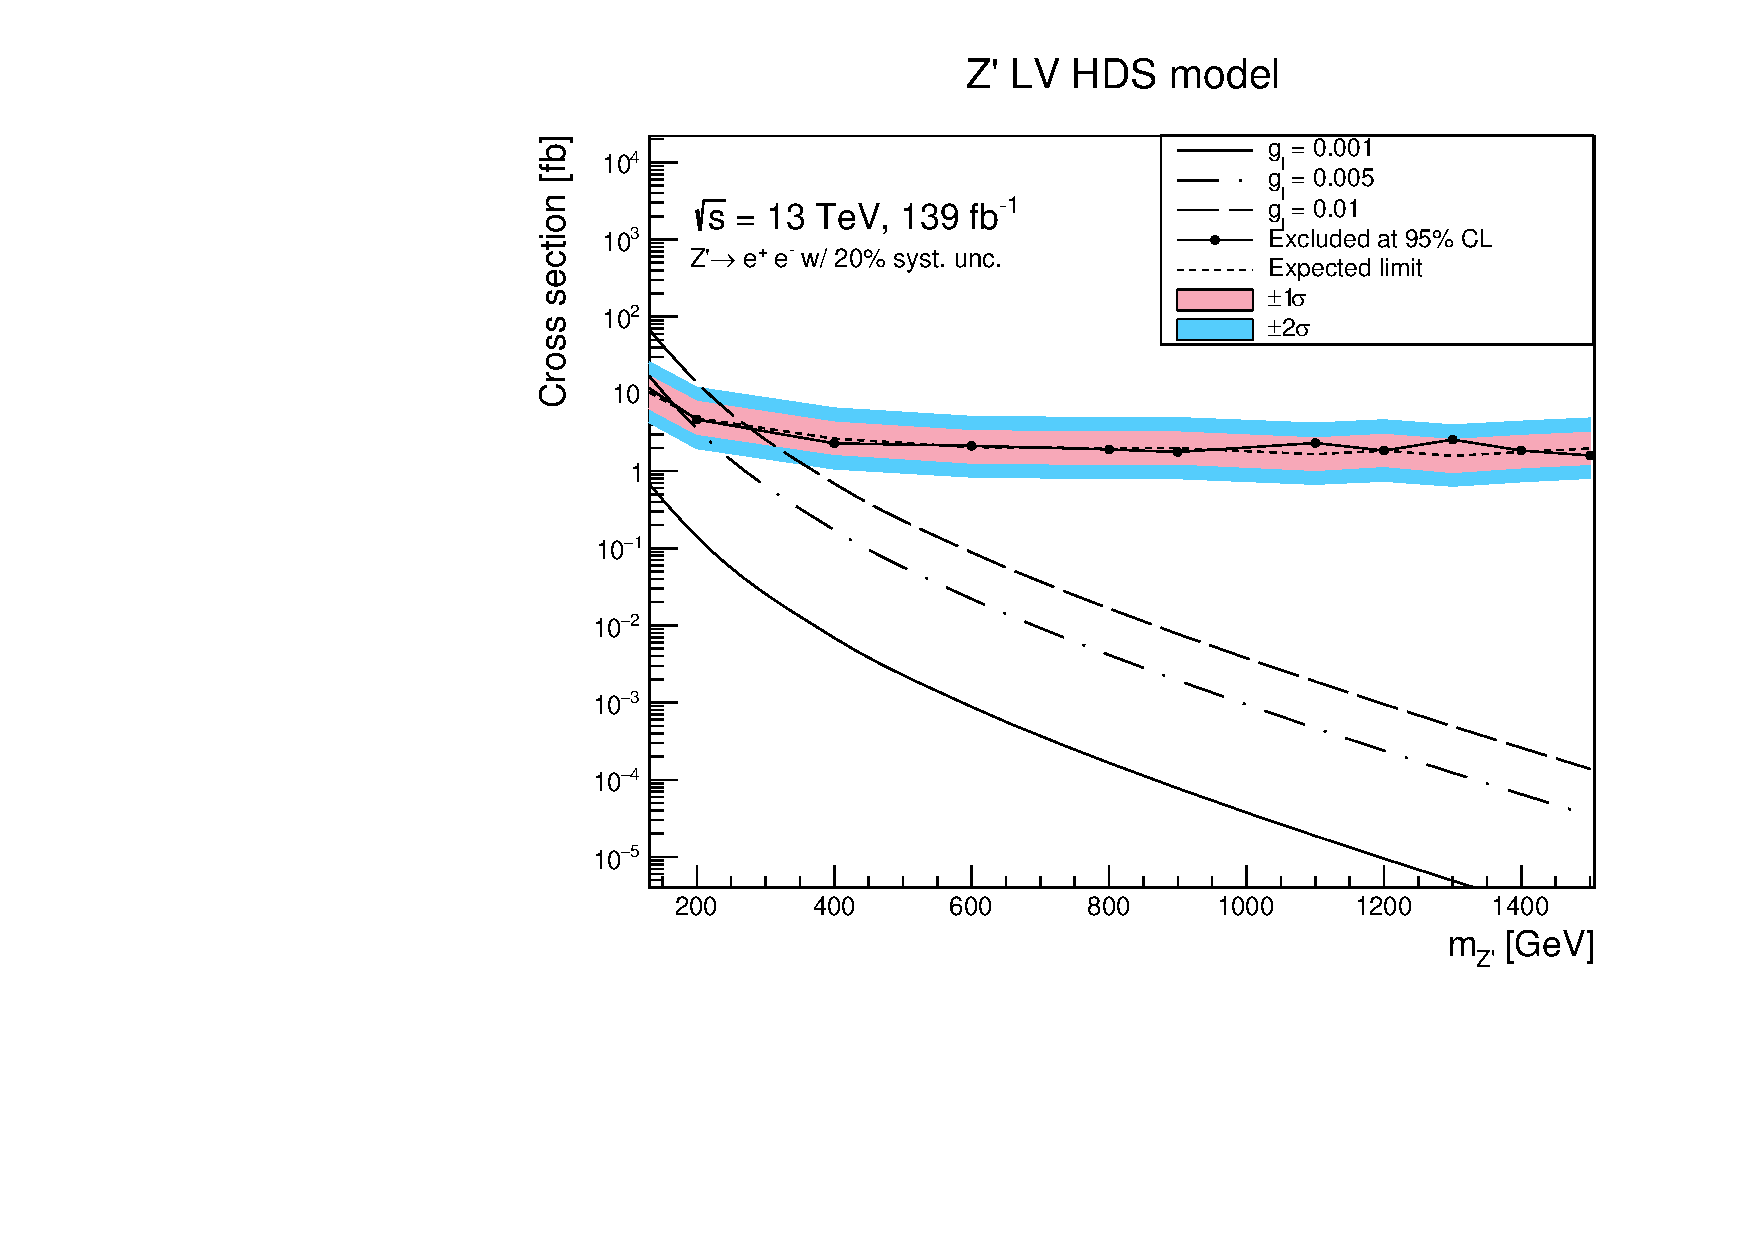
\includegraphics[width=1\textwidth]{Limits/LV_HDS/mass_exclusion_ee.pdf}
      \end{subfigure}
   \hfill
   \begin{subfigure}[b]{0.49\textwidth}
      \centering
      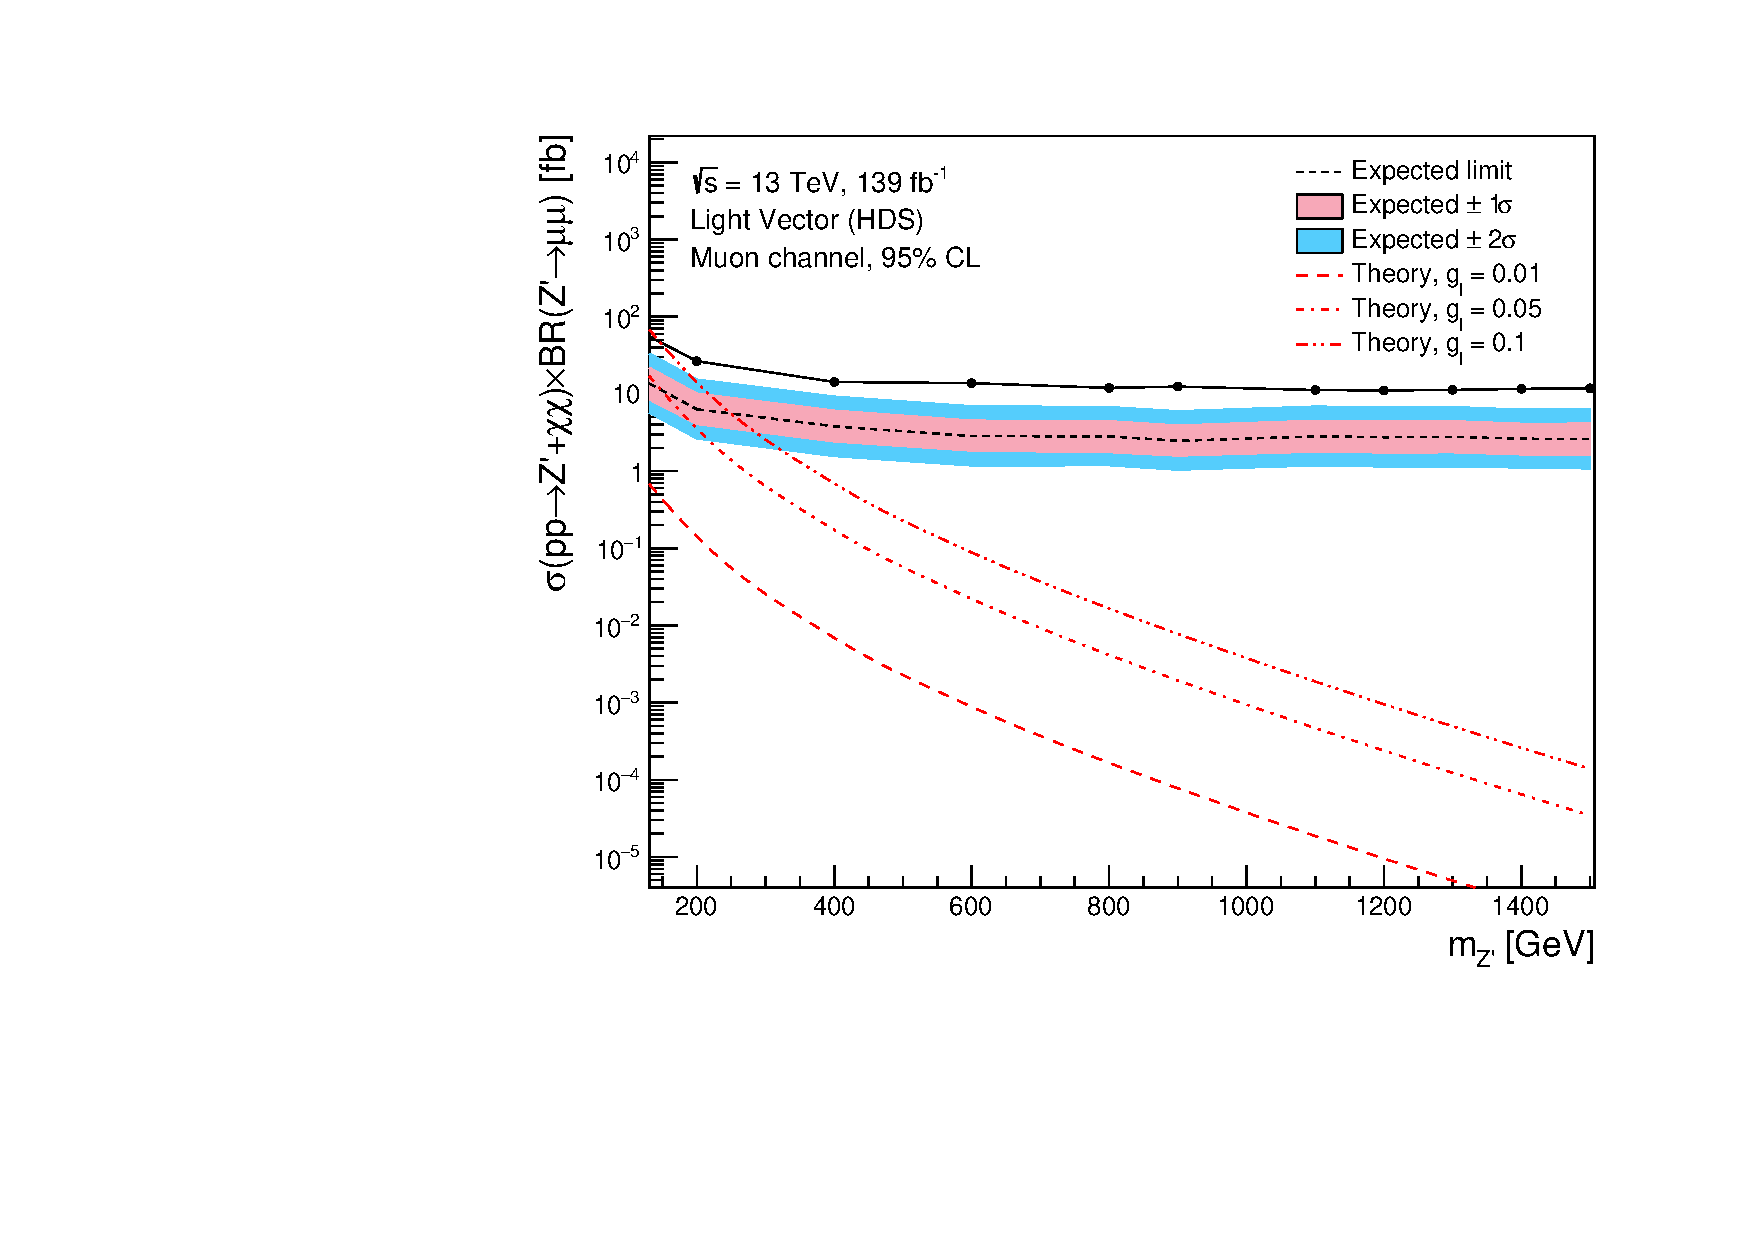
\includegraphics[width=1\textwidth]{Limits/LV_HDS/mass_exclusion_uu.pdf}
      \end{subfigure}
   \caption[Expected mass exclusion limits of $ee$ and $\mu\mu$ channel for all Z' LV HDS model using the model dependent approach]{Mass exclusion limits of $ee$ (left) and $\mu\mu$ (right) channel for Z' Light Vector Heavy Dark Sector model using the model dependent approach. The y-axis of both plots represents the cross-section times branching ratio of the process we are studying. The x-axis is the mass of the $Z'$ boson. We did not interpolate between the available masses we had simulated, 
   and have rather just connected the values calculated for each mass point by connecting the points. The dashed black line is the expected 95\% CL limit with a 1$\sigma$ and 2$\sigma$ variance. 
   The different red dashed lines represent the theoretical cross-section times branching ratio of the process when varying the value of the lepton coupling $g_l$ between the leptons and the $Z'$ boson. The simulated events in this thesis utilized the value $g_l=$ 0.01, we include the cross-section times branching ratio when increasing this coupling to 0.05 and 0.1 to see how the exclusions change.  }\label{fig:LV_HDS_exclusion_ee_uu}
\end{figure}

\begin{figure}[!ht]
	\centering
	\begin{subfigure}[b]{0.49\textwidth}
      \centering
      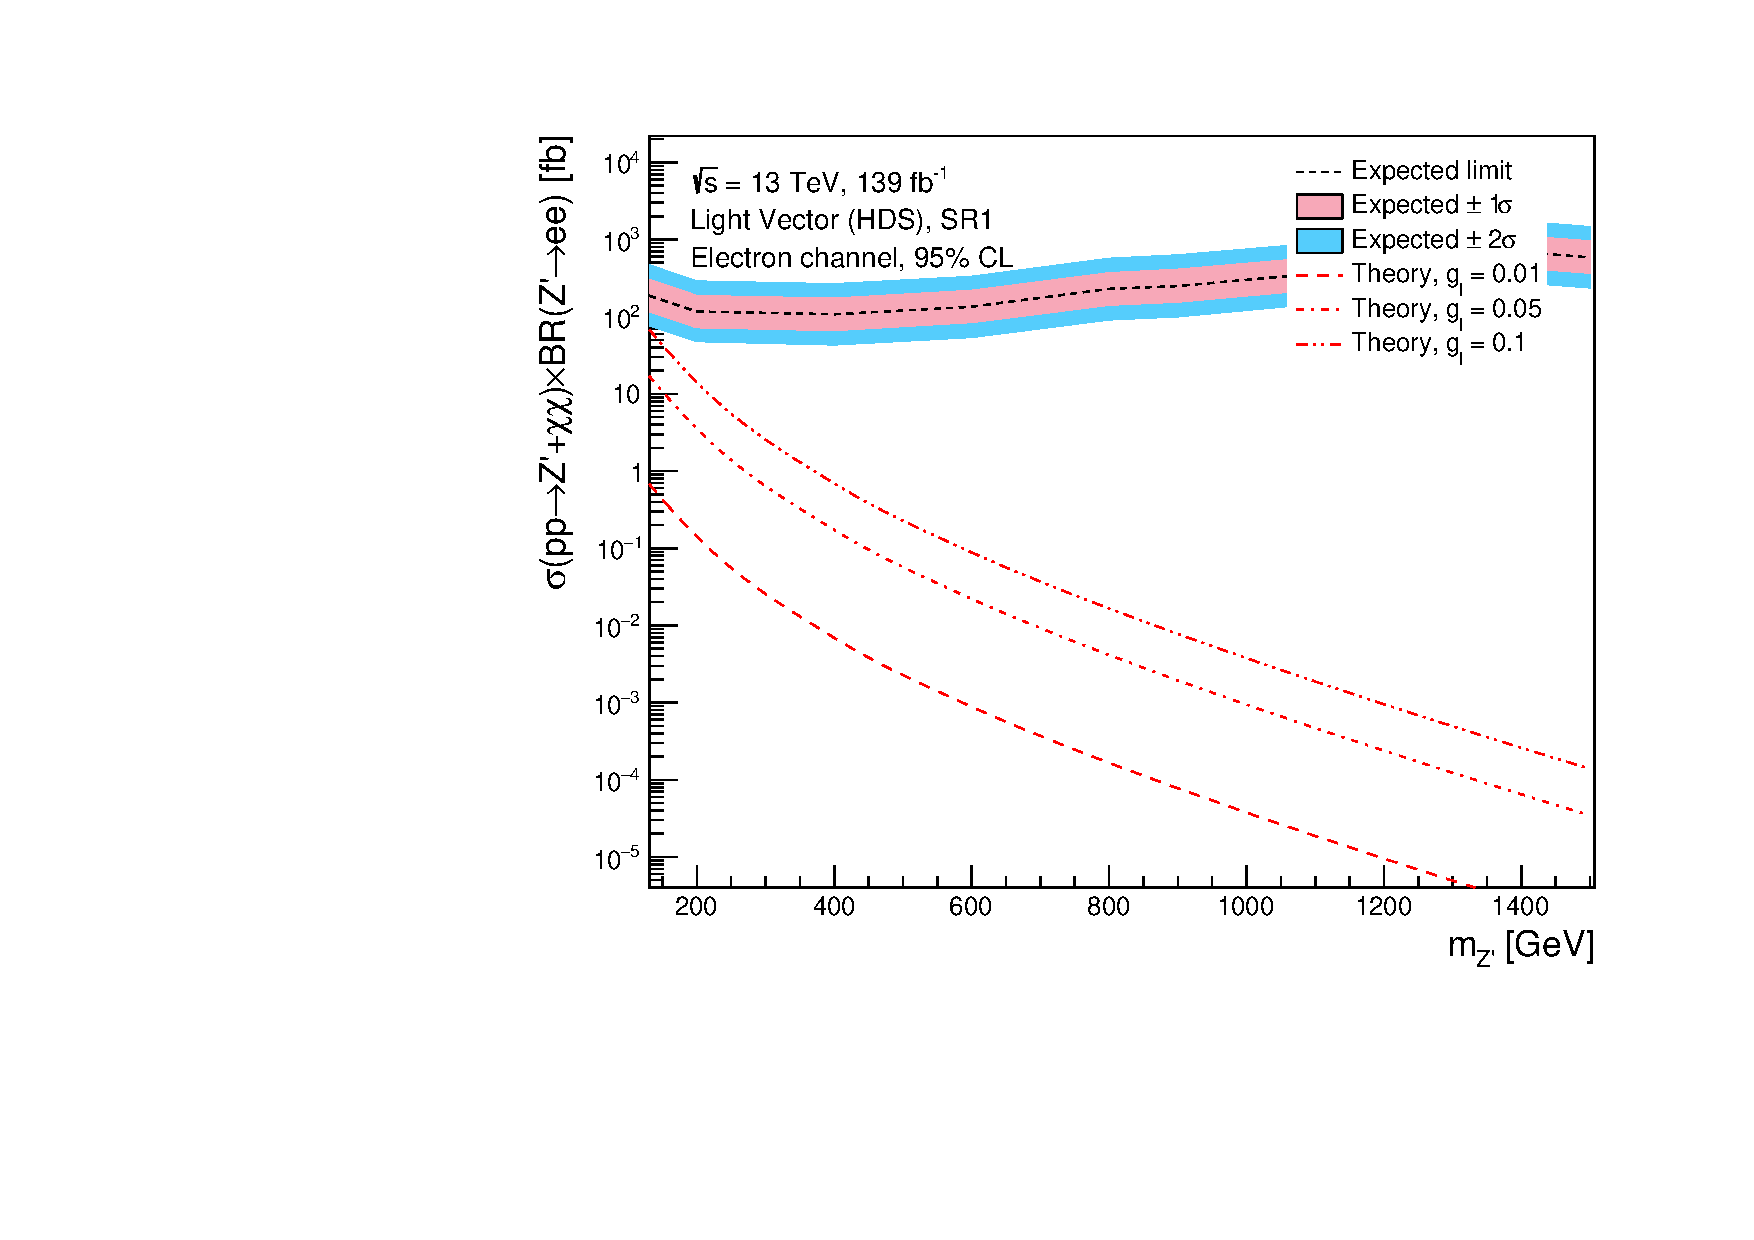
\includegraphics[width=1\textwidth]{Limits/Model_independent/50-100/LV_HDS/mass_exclusion_ee.pdf}
   \end{subfigure}
   \hfill
   \begin{subfigure}[b]{0.49\textwidth}
      \centering
      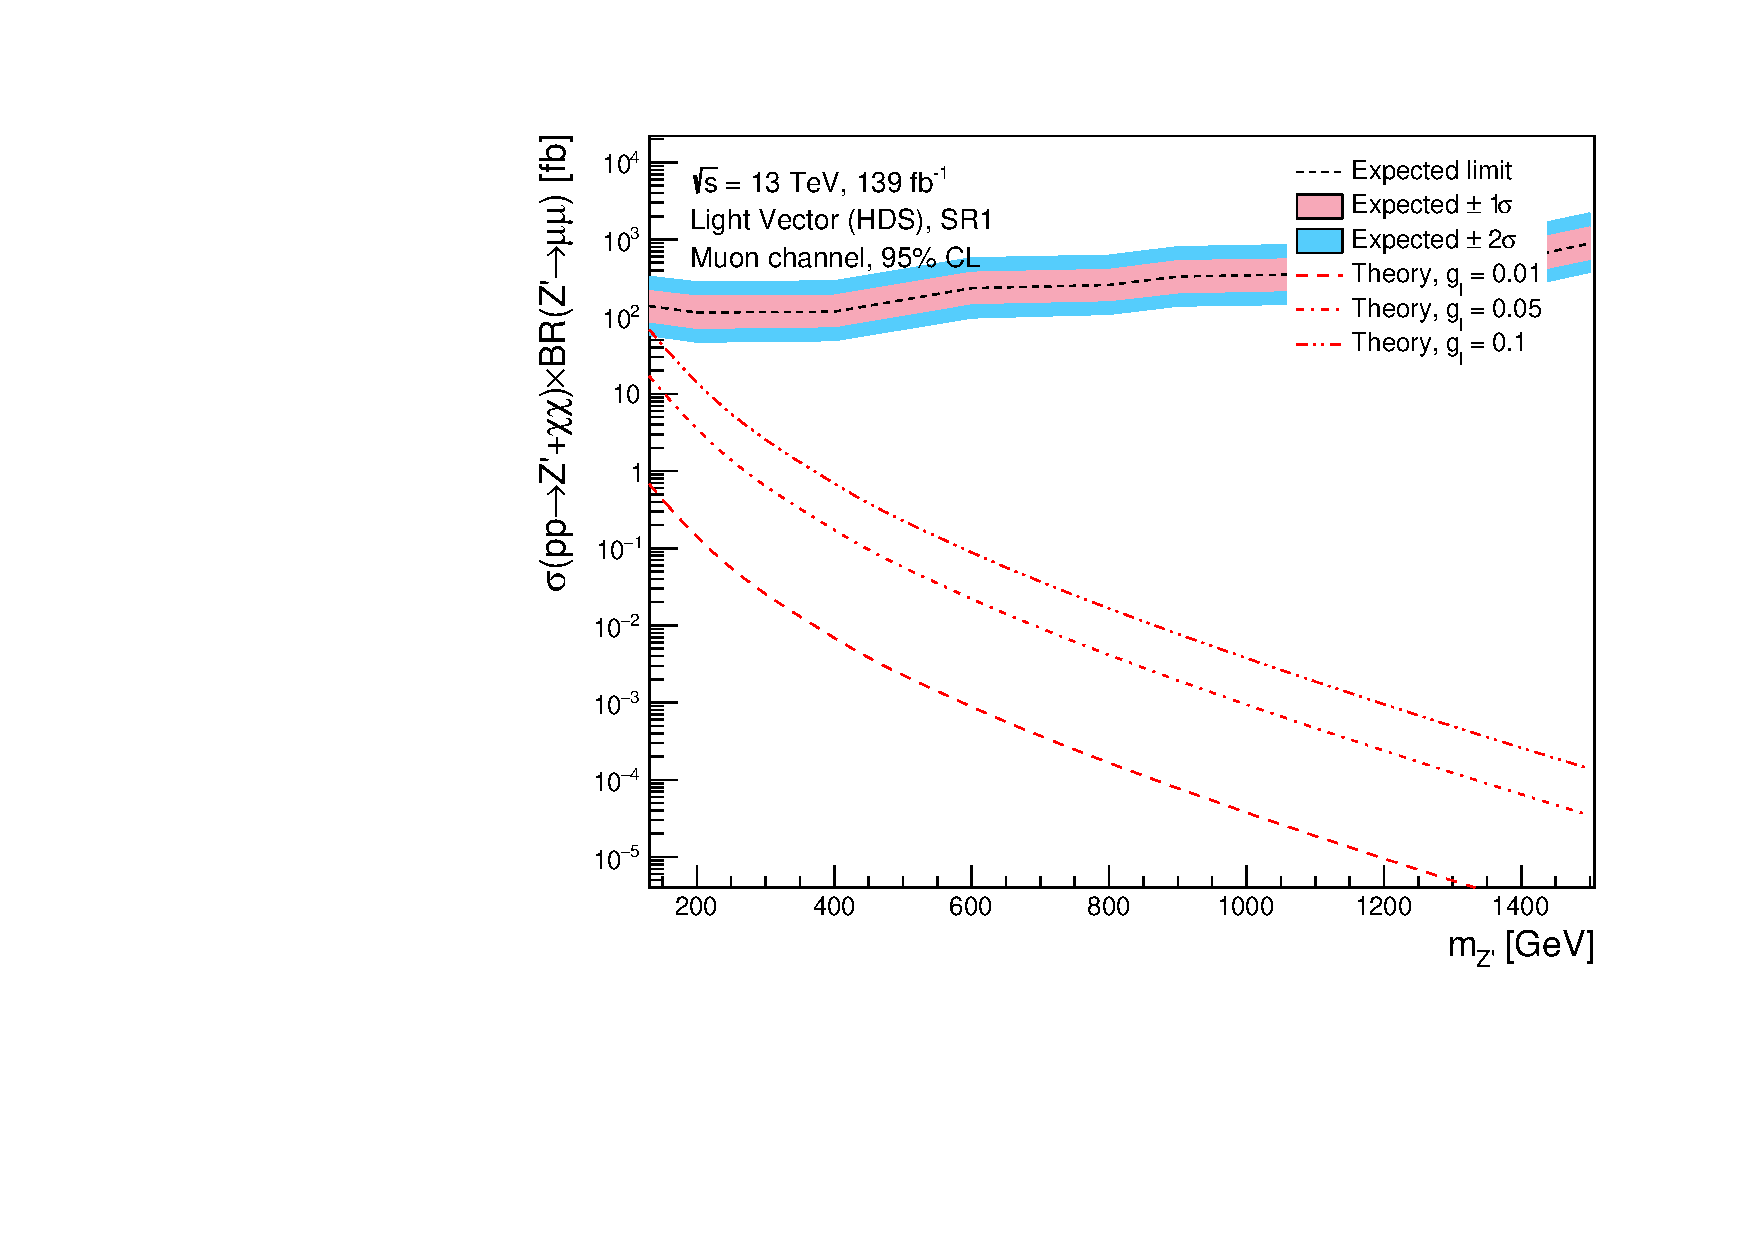
\includegraphics[width=1\textwidth]{Limits/Model_independent/50-100/LV_HDS/mass_exclusion_uu.pdf}
   \end{subfigure}
   \hfill
   \begin{subfigure}[b]{0.49\textwidth}
      \centering
      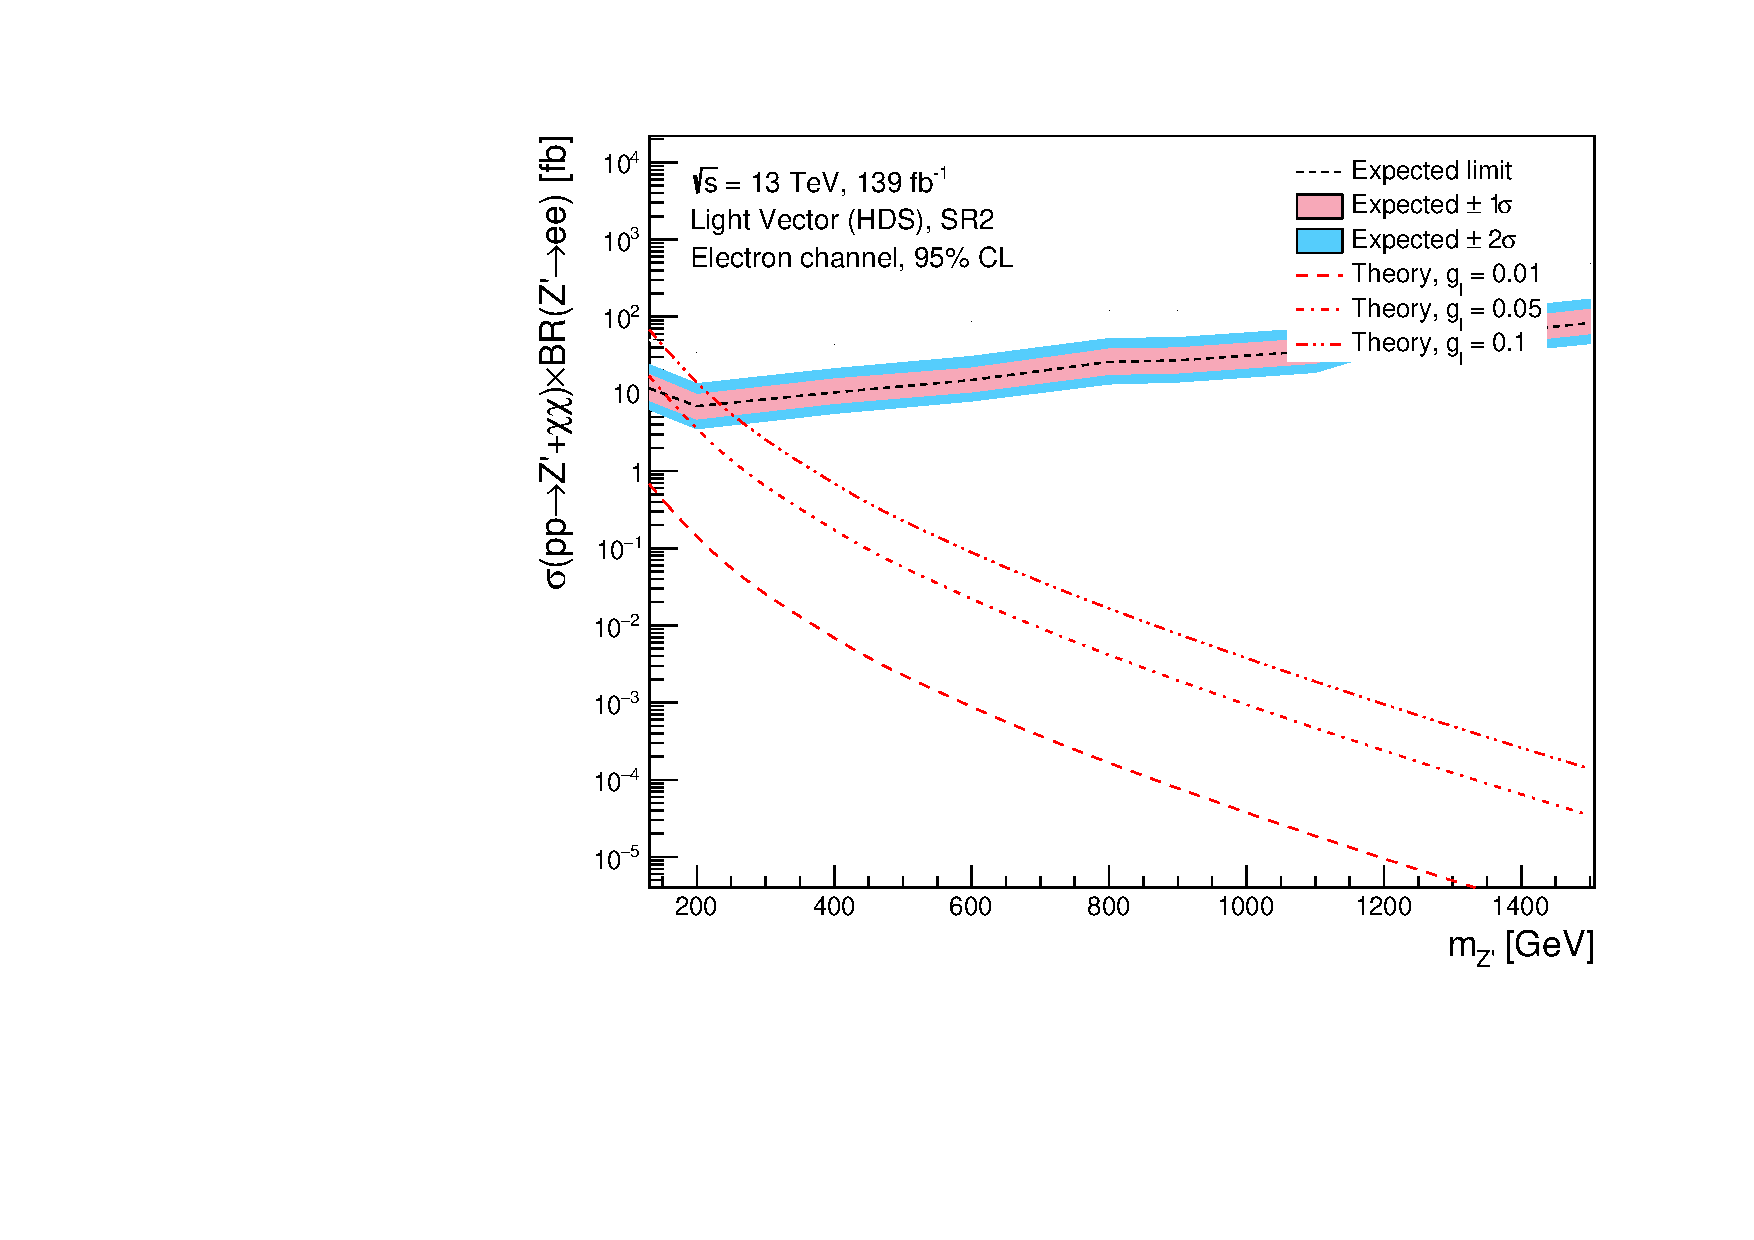
\includegraphics[width=1\textwidth]{Limits/Model_independent/100-150/LV_HDS/mass_exclusion_ee.pdf}
   \end{subfigure}
   \hfill
   \begin{subfigure}[b]{0.49\textwidth}
      \centering
      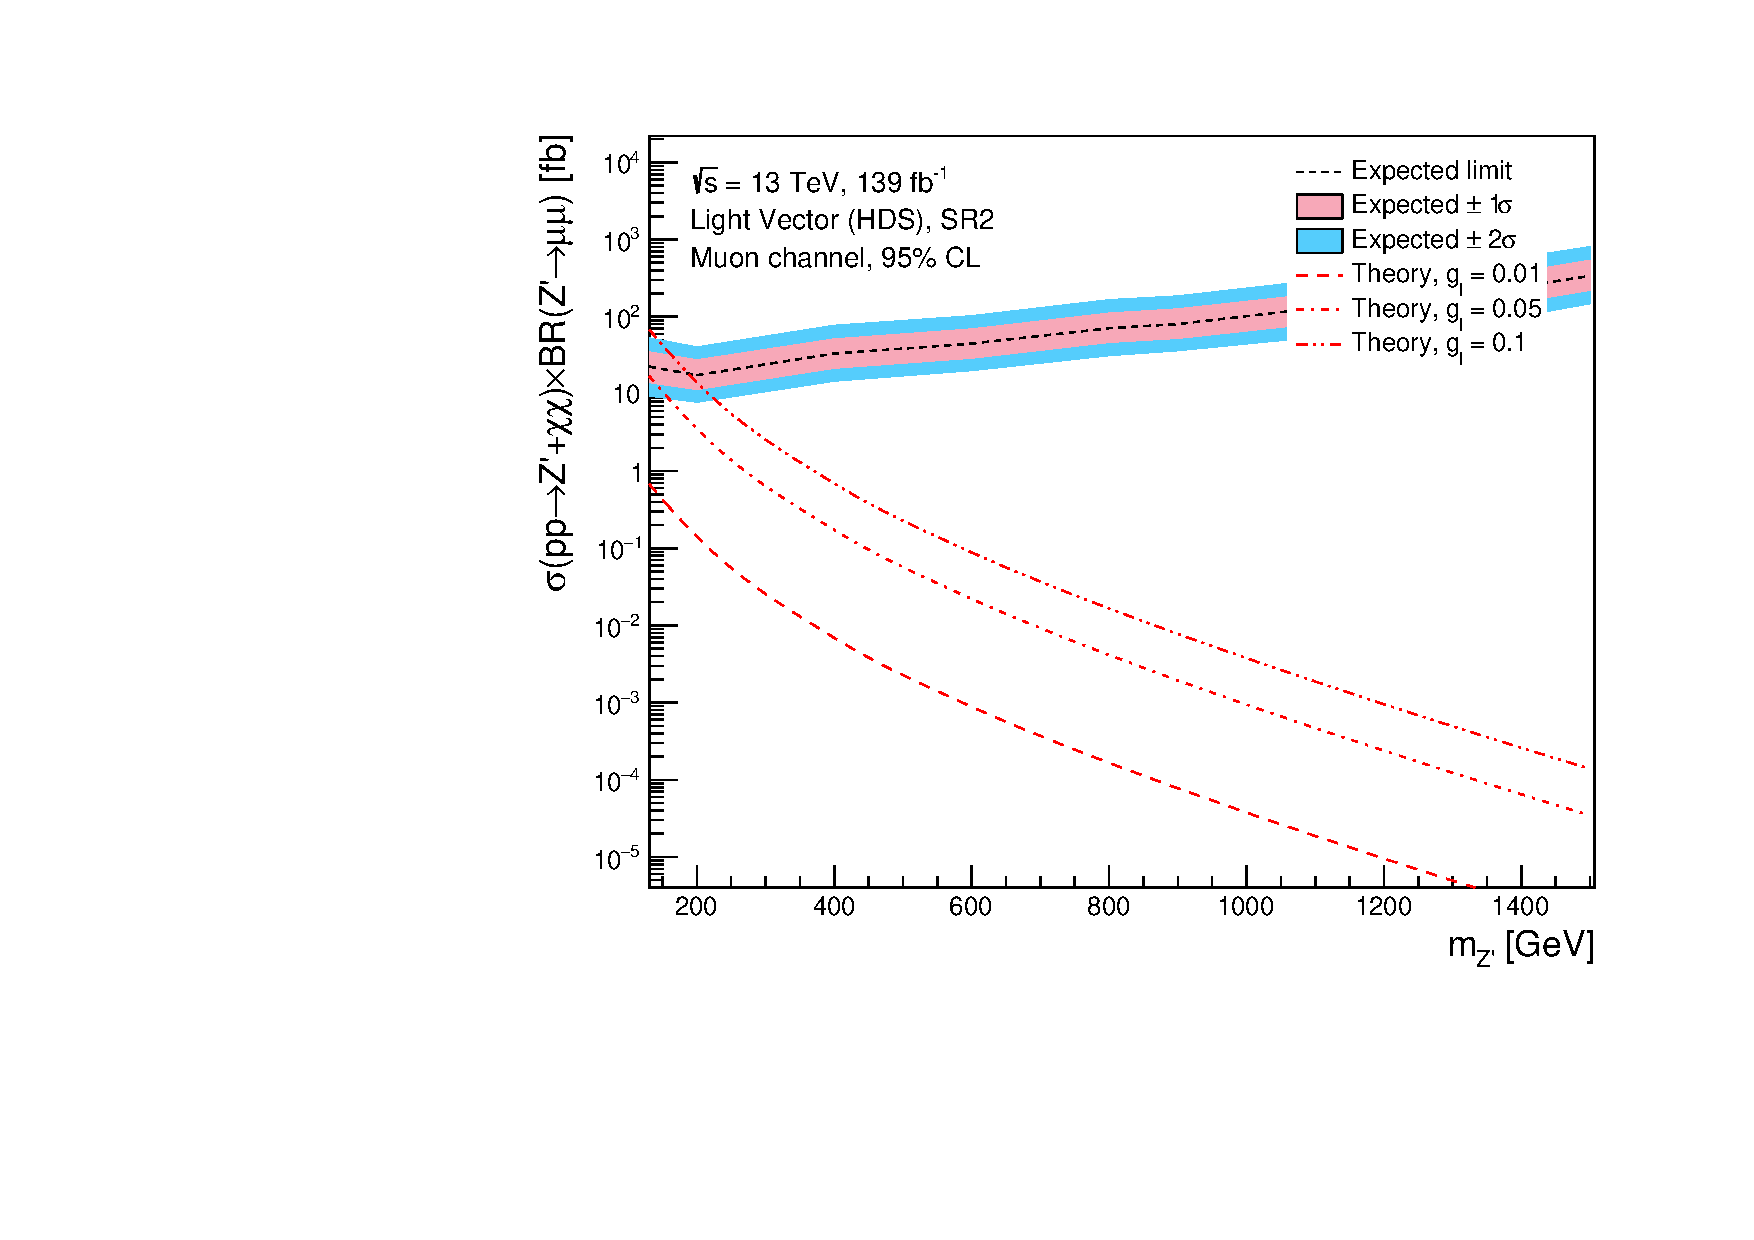
\includegraphics[width=1\textwidth]{Limits/Model_independent/100-150/LV_HDS/mass_exclusion_uu.pdf}
   \end{subfigure}
   \hfill
	\begin{subfigure}[b]{0.49\textwidth}
      \centering
      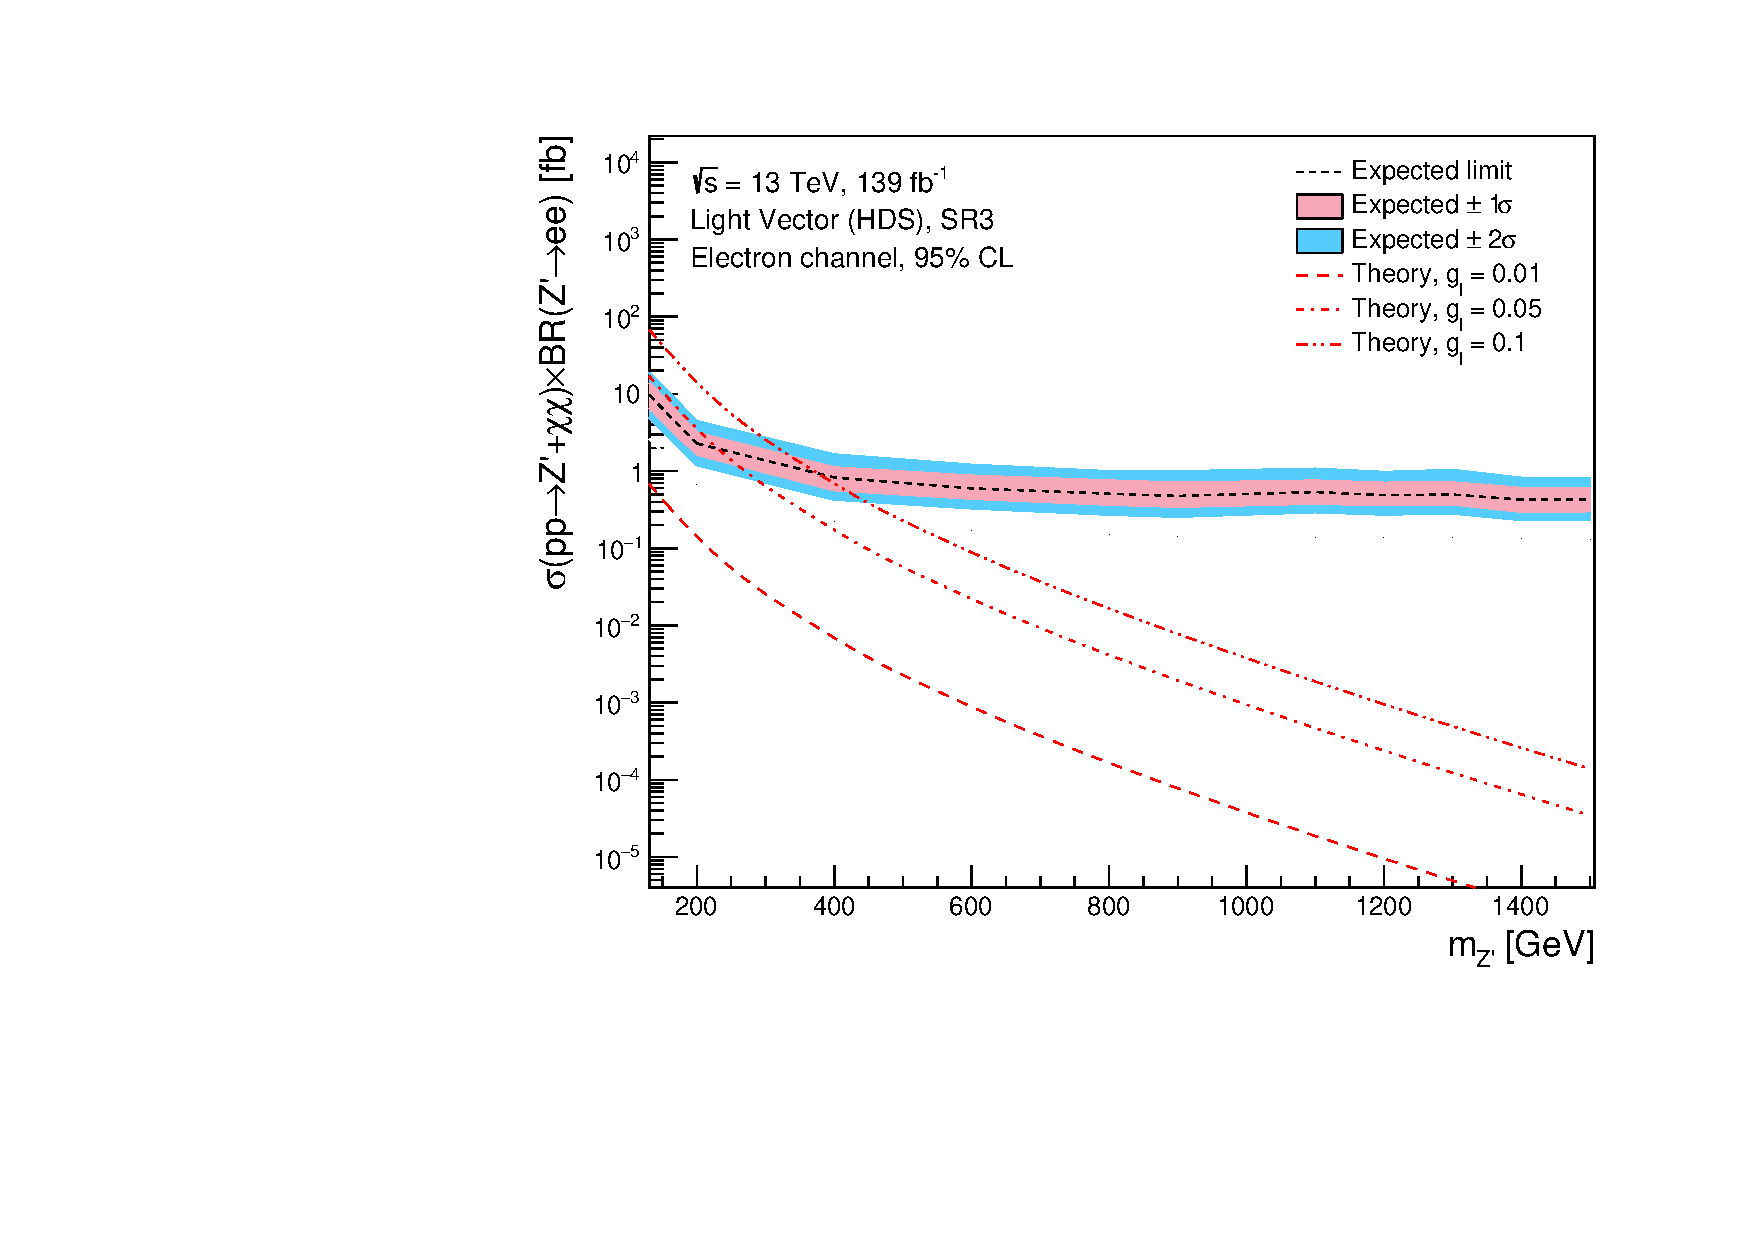
\includegraphics[width=1\textwidth]{Limits/Model_independent/150/LV_HDS/mass_exclusion_ee.pdf}
   \end{subfigure}
   \hfill
   \begin{subfigure}[b]{0.49\textwidth}
      \centering
      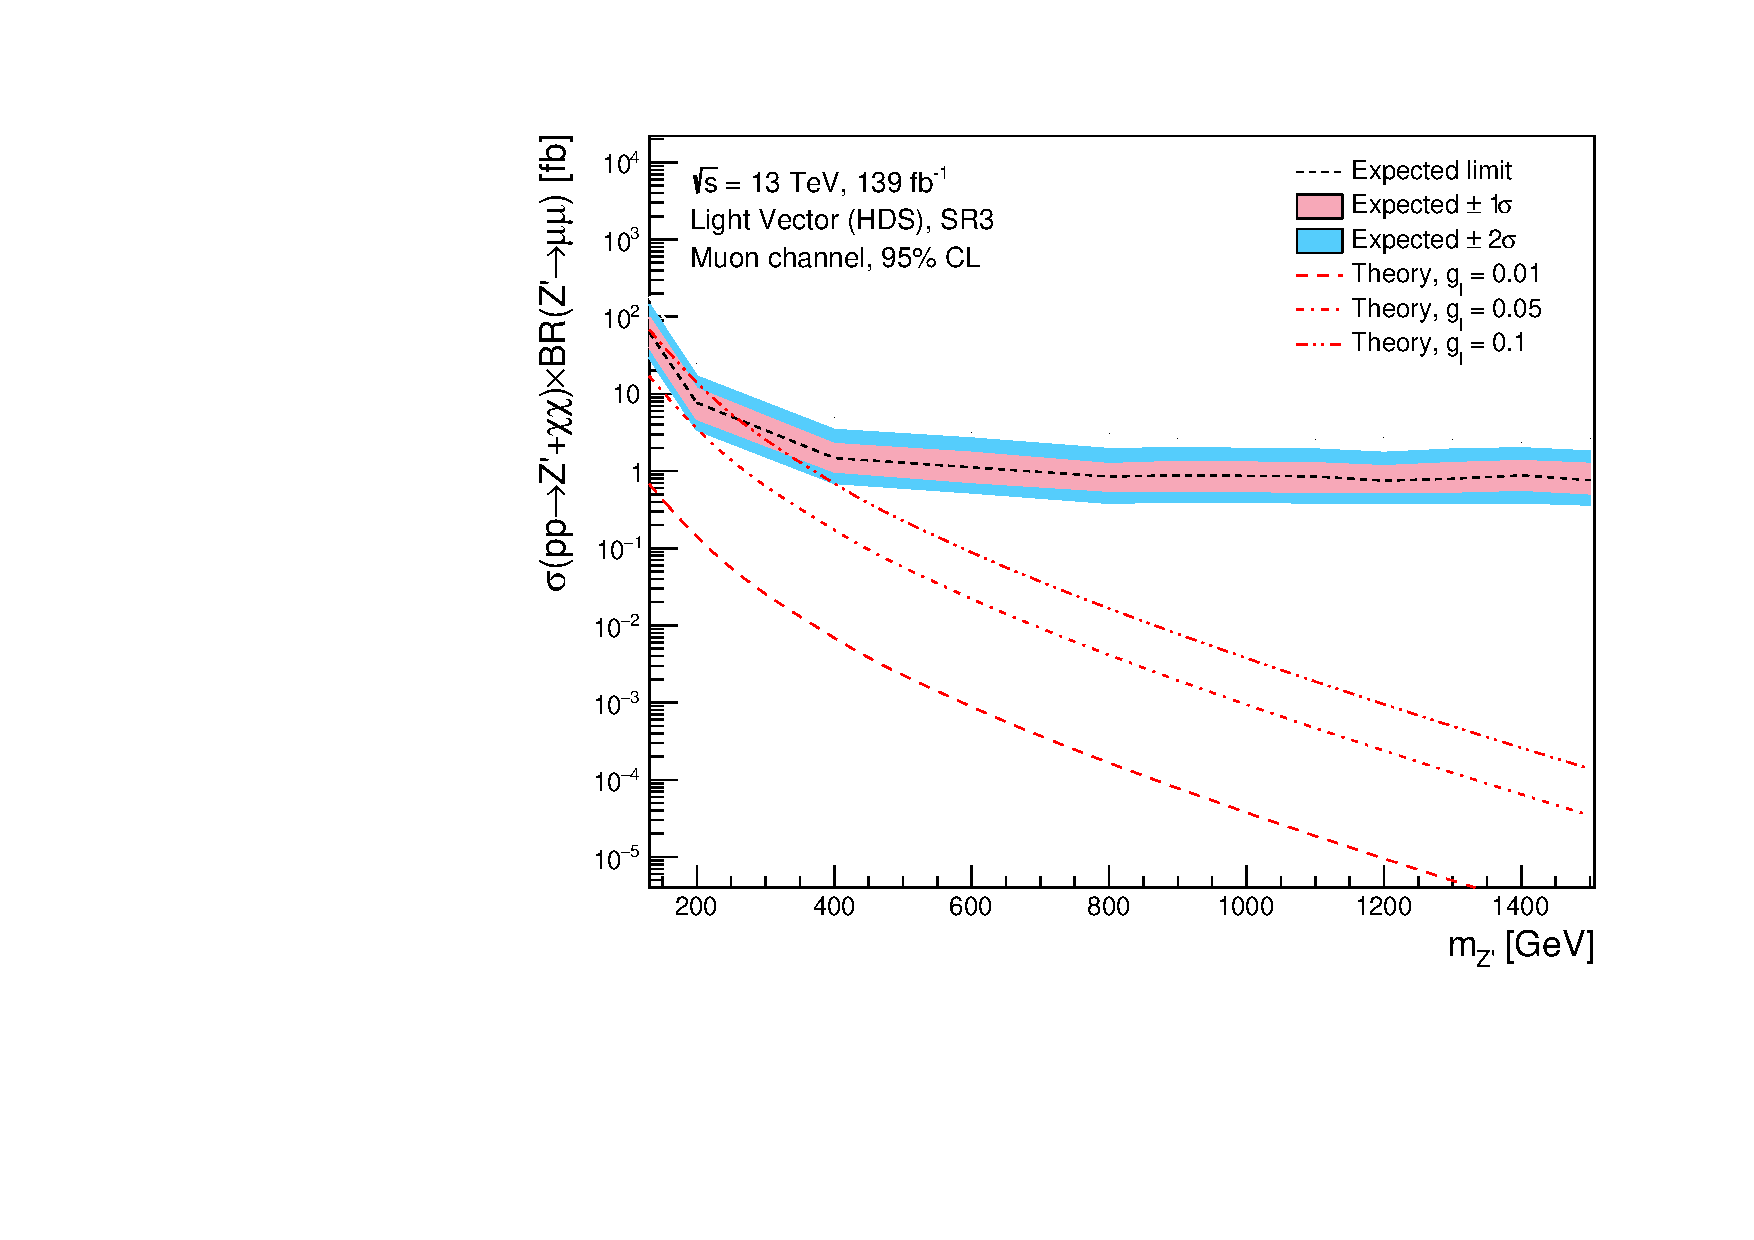
\includegraphics[width=1\textwidth]{Limits/Model_independent/150/LV_HDS/mass_exclusion_uu.pdf}
   \end{subfigure}
   \caption[Expected mass exclusion limits results for LV HDS model on $ee$ and $\mu\mu$ channel using the model independent approach]{Mass exclusion limits of $ee$ (left) and $\mu\mu$ (right) channel for Z' Light Vector Heavy Dark Sector model using the model independent approach. To remind what the SRs are: SR1 has $E_T^{miss}\in[50, 100]$ GeV, SR2 has $E_T^{miss}\in[100, 150]$ GeV, and SR3 has $E_T^{miss}>150$ GeV. The y-axis of both plots represents the cross-section times branching ratio of the process we are studying. The x-axis is the mass of the $Z'$ boson. We did not interpolate between the available masses we had simulated, 
   and have rather just connected the values calculated for each mass point by connecting the points. The dashed black line is the expected 95\% CL limit with a 1$\sigma$ and 2$\sigma$ variance. 
   The different red dashed lines represent the theoretical cross-section times branching ratio of the process when varying the value of the lepton coupling $g_l$ between the leptons and the $Z'$ boson. The simulated events in this thesis utilized the value $g_l=$ 0.01, we include the cross-section times branching ratio when increasing this coupling to 0.05 and 0.1 to see how the exclusions change.  }\label{fig:LV_HDS_me_SRS}
\end{figure}


\clearpage
\section{Light Vector Light Dark Sector}
\begin{figure}[!ht]
	\centering
   \begin{subfigure}[b]{0.49\textwidth}
      \centering
      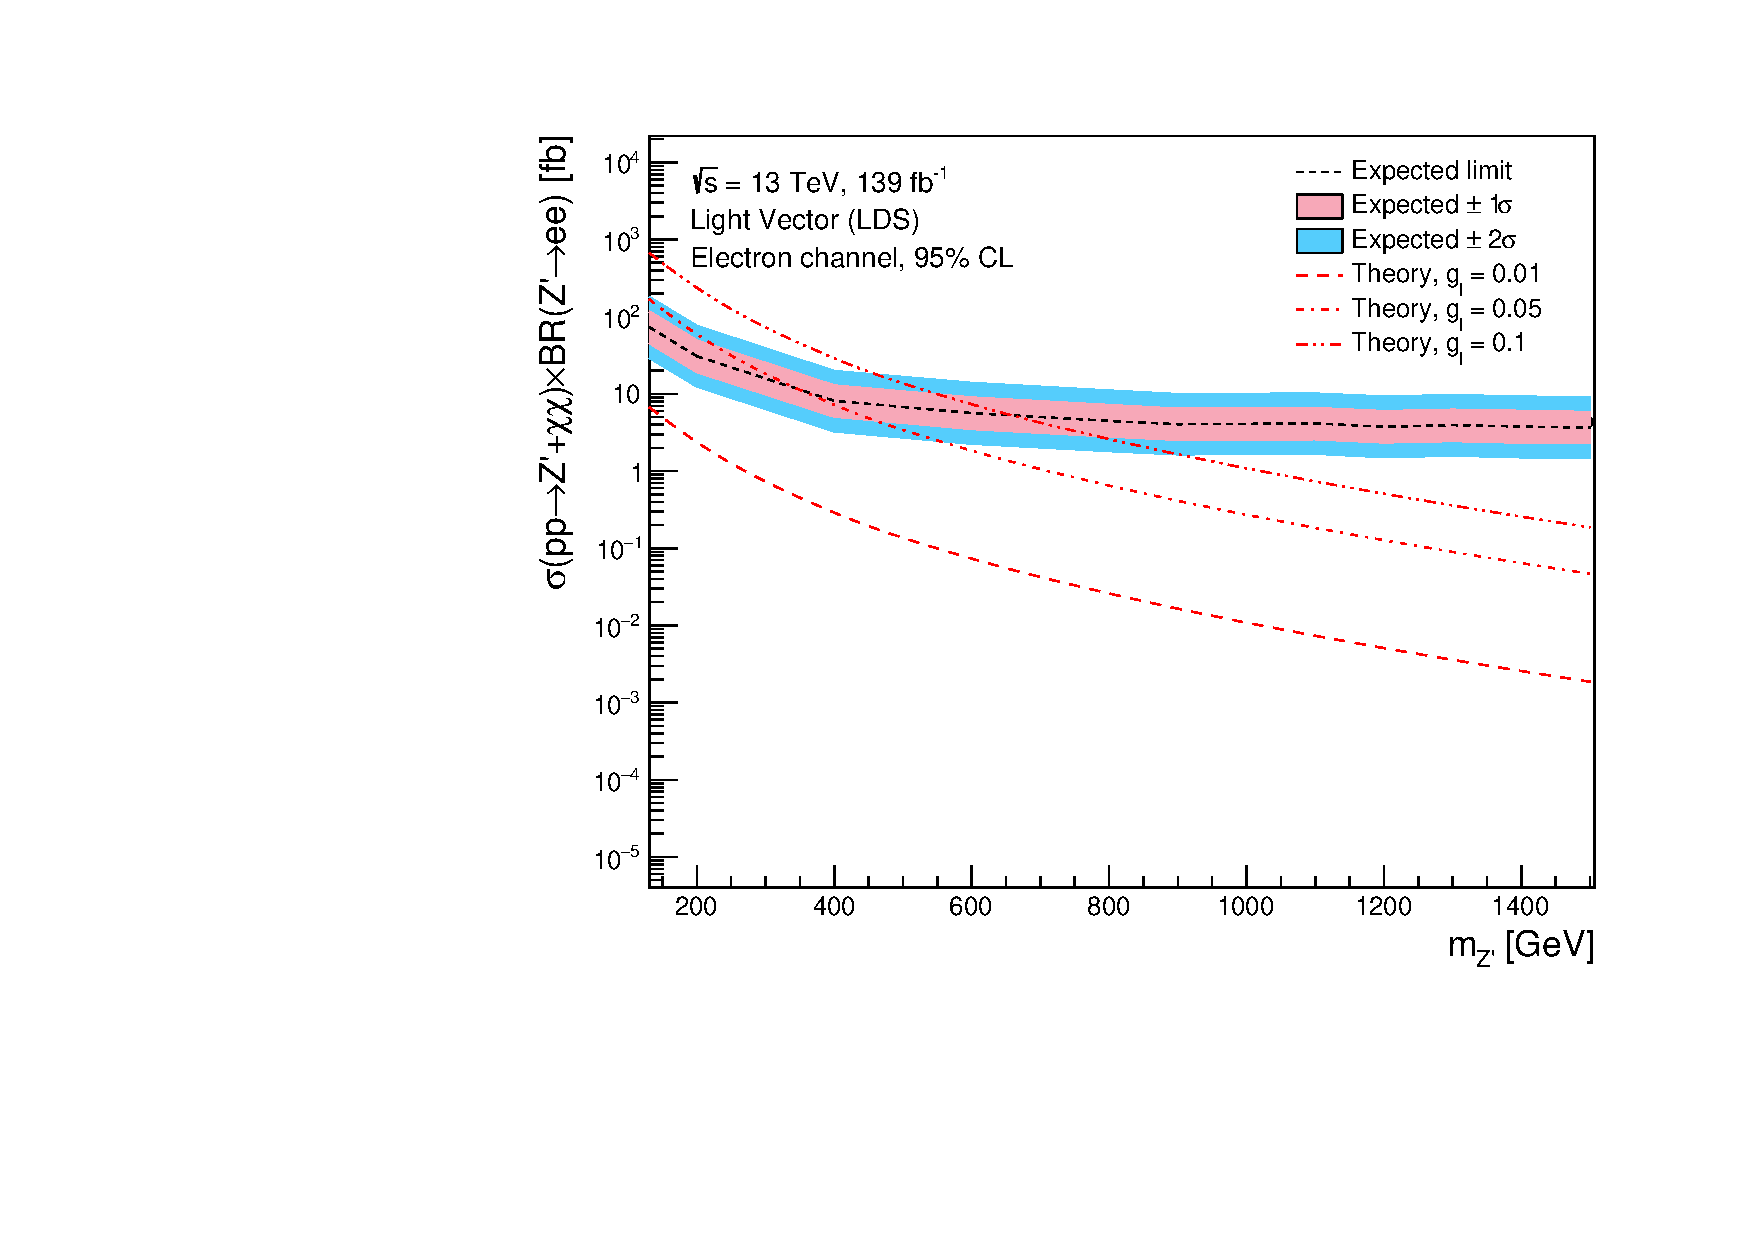
\includegraphics[width=1\textwidth]{Limits/LV_LDS/mass_exclusion_ee.pdf}
      \end{subfigure}
   \hfill
   \begin{subfigure}[b]{0.49\textwidth}
      \centering
      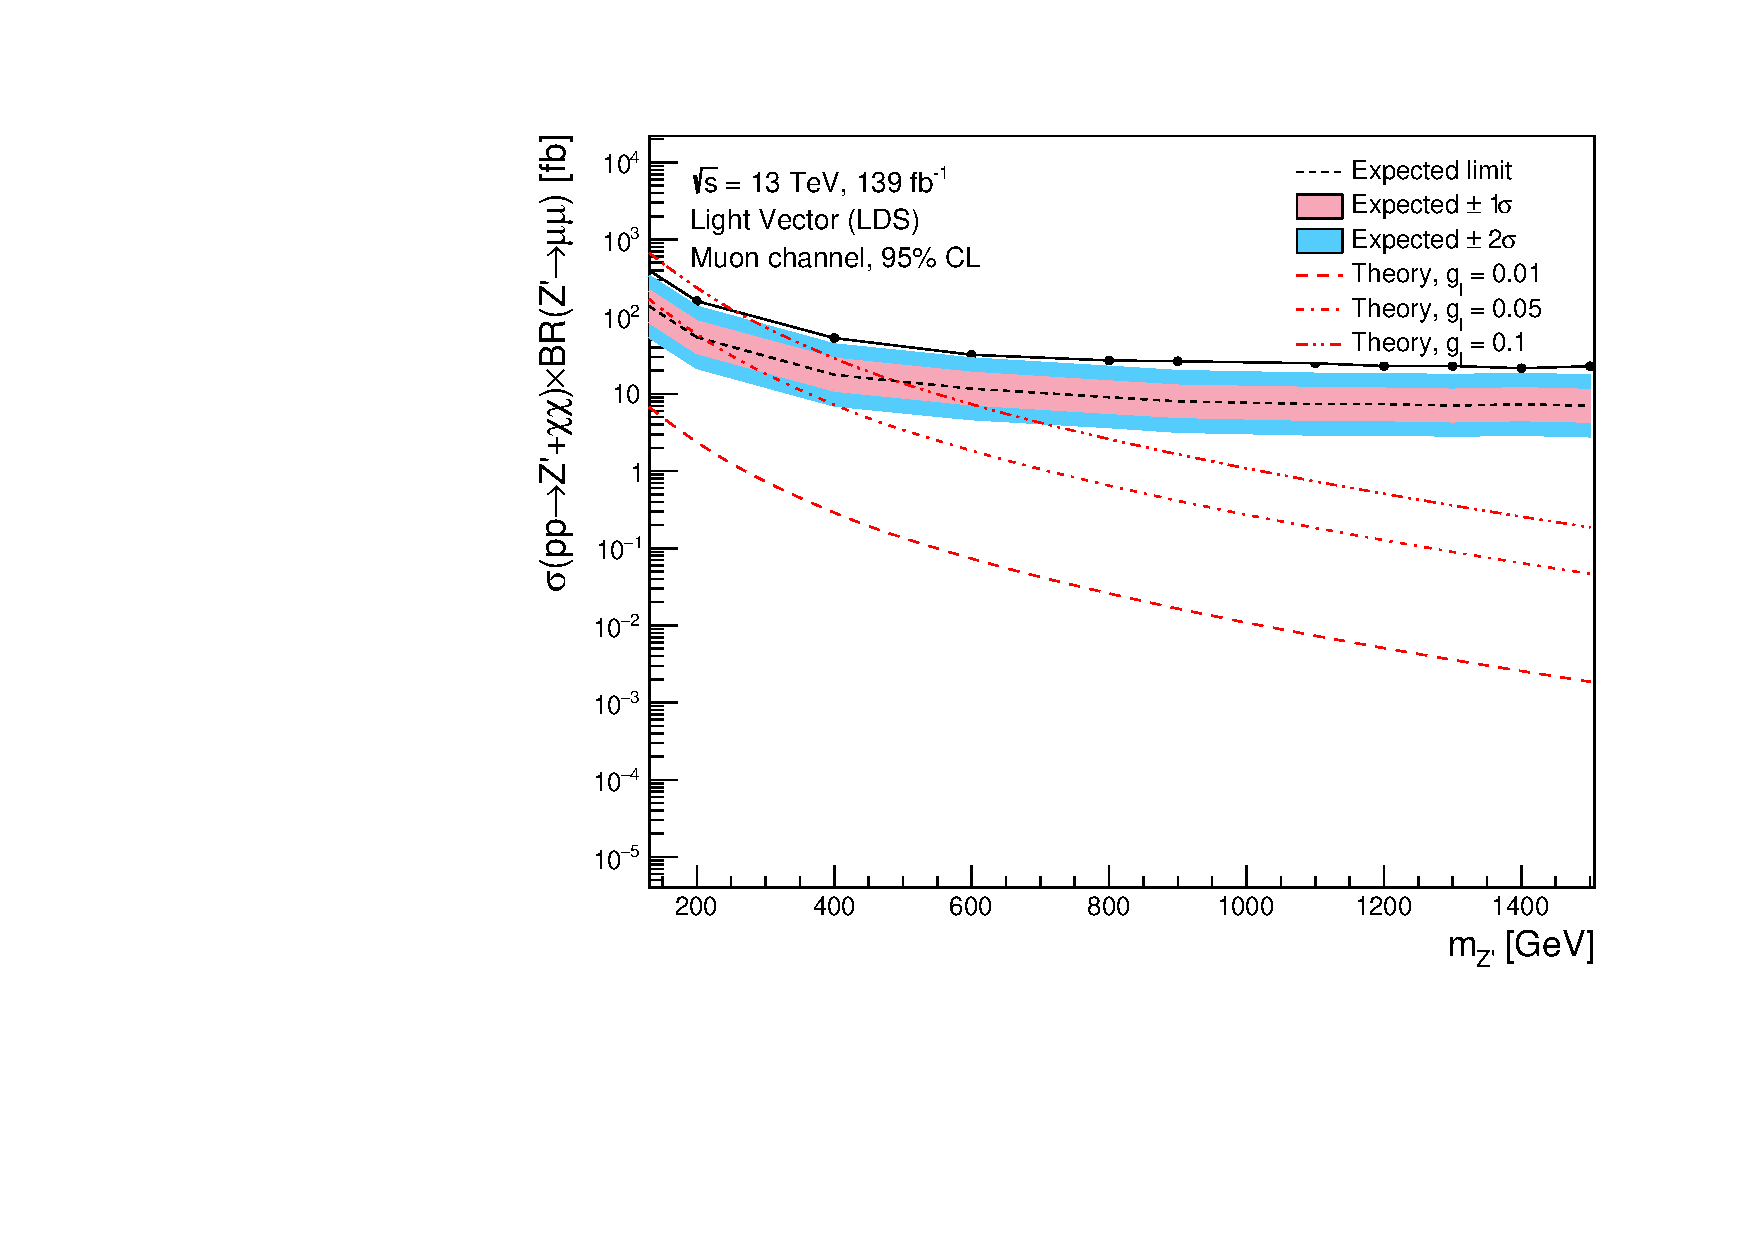
\includegraphics[width=1\textwidth]{Limits/LV_LDS/mass_exclusion_uu.pdf}
      \end{subfigure}
   \caption[Expected mass exclusion limits of $ee$ and $\mu\mu$ channel for all Z' LV LDS model using the model dependent approach]{Mass exclusion limits of $ee$ (left) and $\mu\mu$ (right) channel for Z' Light Vector Light Dark Sector model using the model dependent approach. The y-axis of both plots represents the cross-section times branching ratio of the process we are studying. The x-axis is the mass of the $Z'$ boson. We did not interpolate between the available masses we had simulated, 
   and have rather just connected the values calculated for each mass point by connecting the points. The dashed black line is the expected 95\% CL limit with a 1$\sigma$ and 2$\sigma$ variance. 
   The different red dashed lines represent the theoretical cross-section times branching ratio of the process when varying the value of the lepton coupling $g_l$ between the leptons and the $Z'$ boson. The simulated events in this thesis utilized the value $g_l=$ 0.01, we include the cross-section times branching ratio when increasing this coupling to 0.05 and 0.1 to see how the exclusions change.  }\label{fig:LV_LDS_exclusion_ee_uu}
\end{figure}

\begin{figure}[!ht]
	\centering
	\begin{subfigure}[b]{0.49\textwidth}
      \centering
      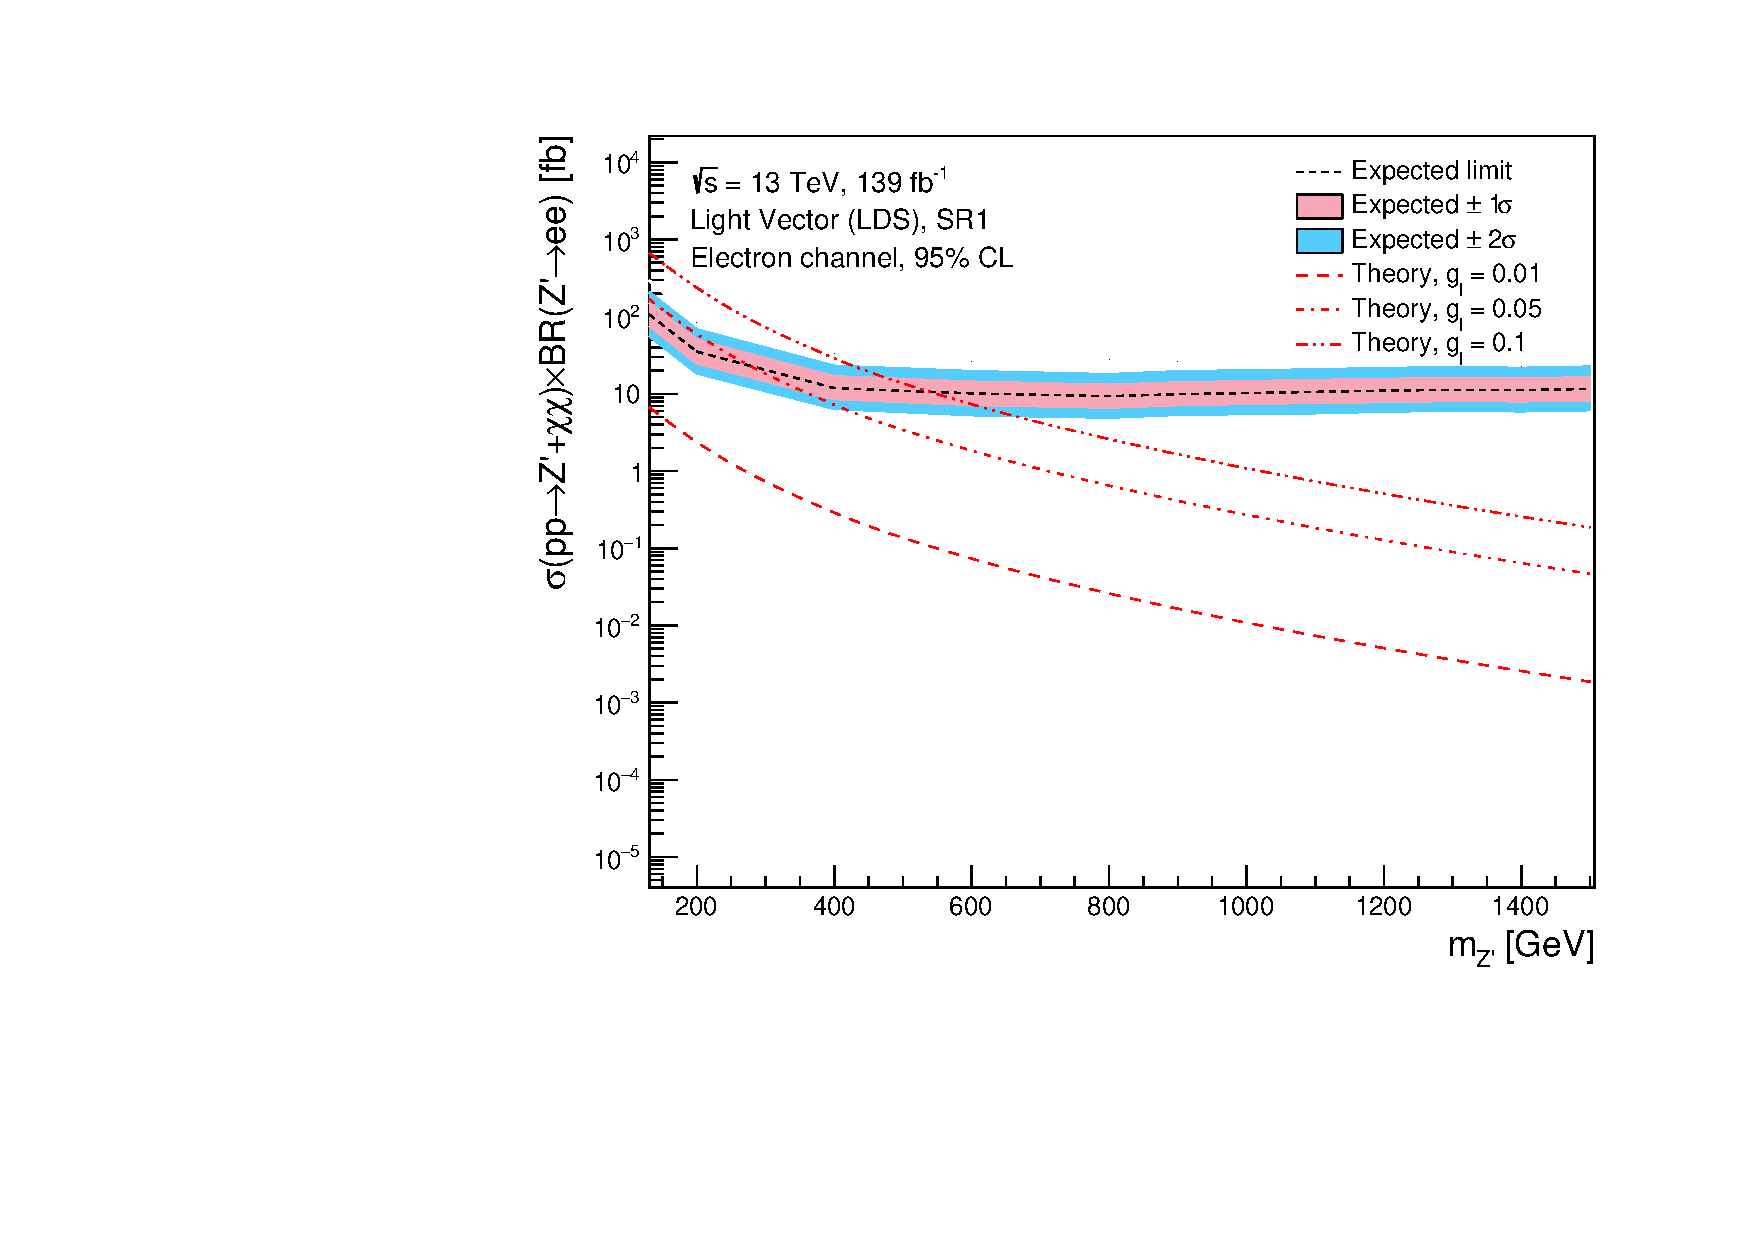
\includegraphics[width=1\textwidth]{Limits/Model_independent/50-100/LV_LDS/mass_exclusion_ee.pdf}
   \end{subfigure}
   \hfill
   \begin{subfigure}[b]{0.49\textwidth}
      \centering
      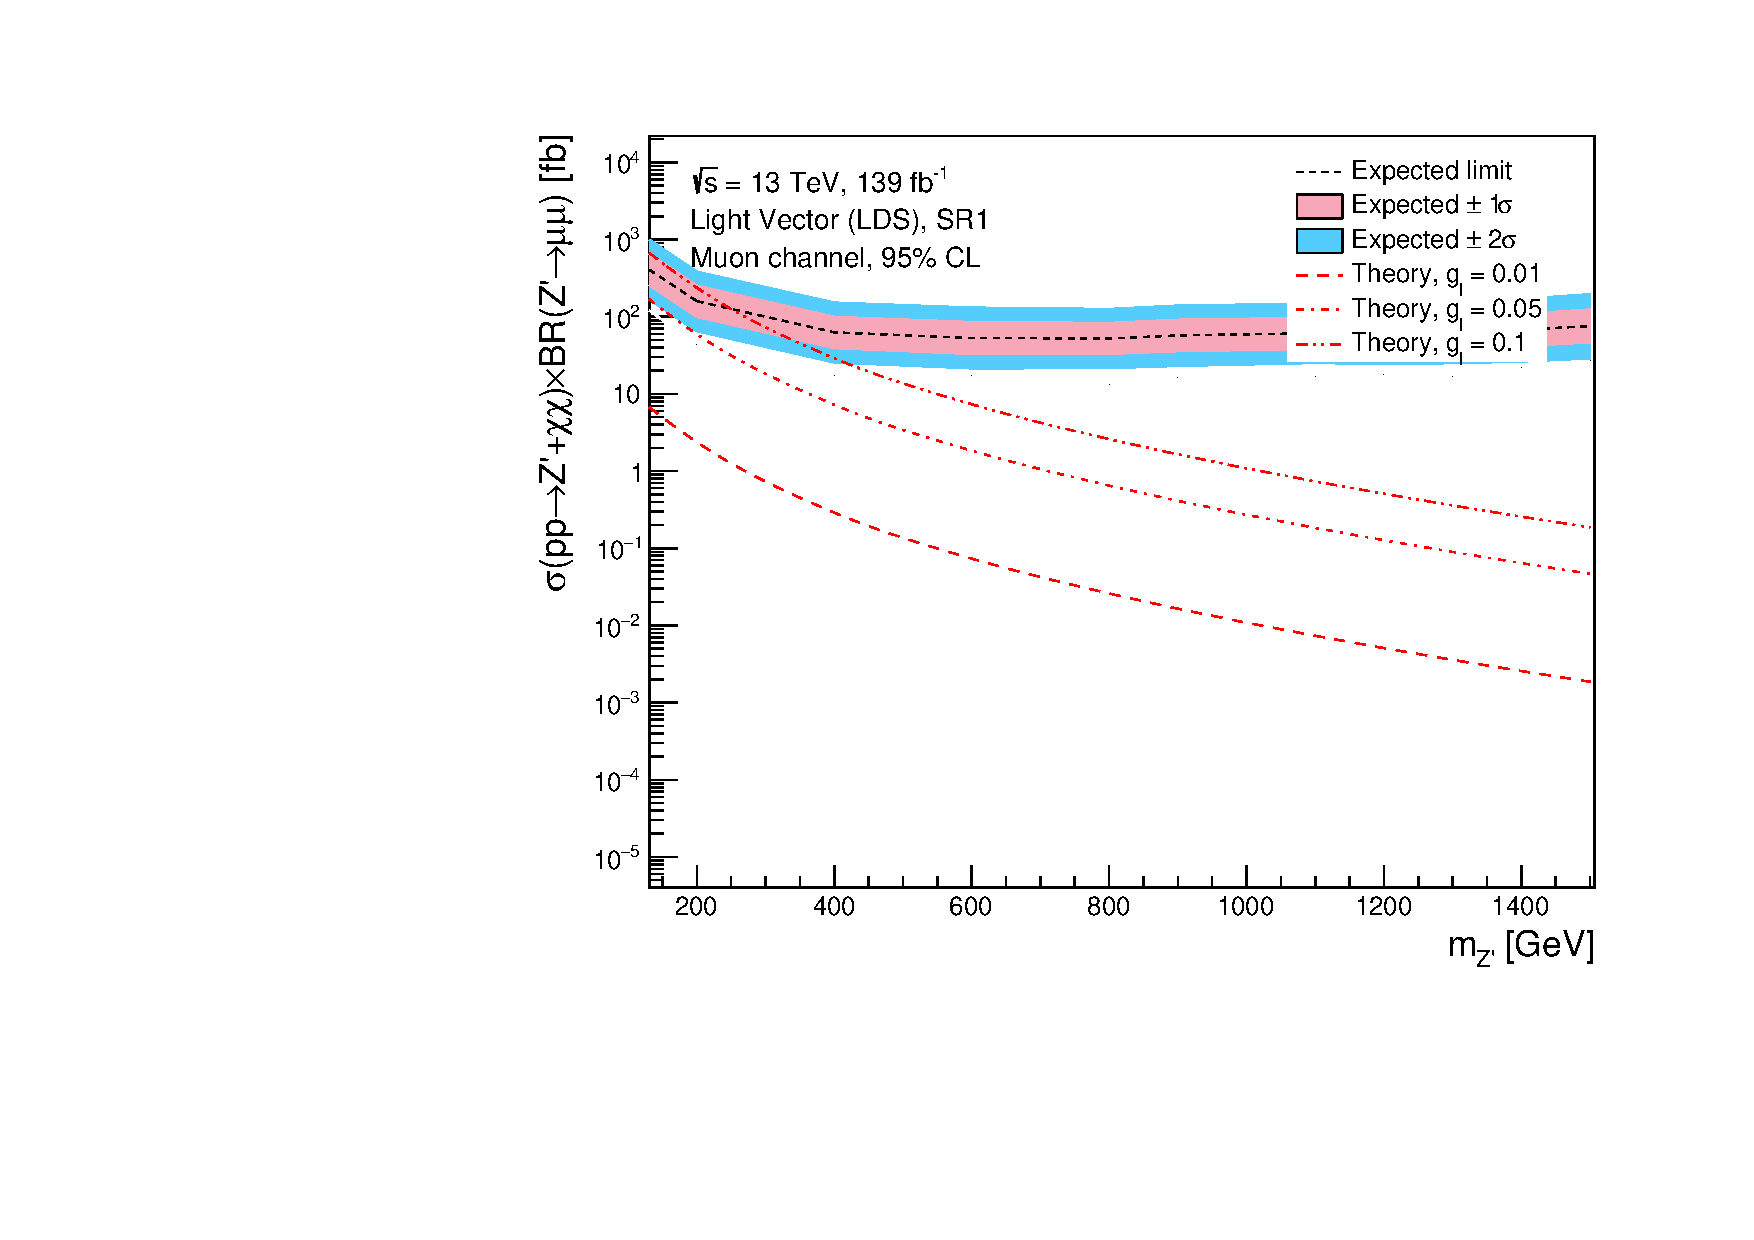
\includegraphics[width=1\textwidth]{Limits/Model_independent/50-100/LV_LDS/mass_exclusion_uu.pdf}
   \end{subfigure}
   \hfill
   \begin{subfigure}[b]{0.49\textwidth}
      \centering
      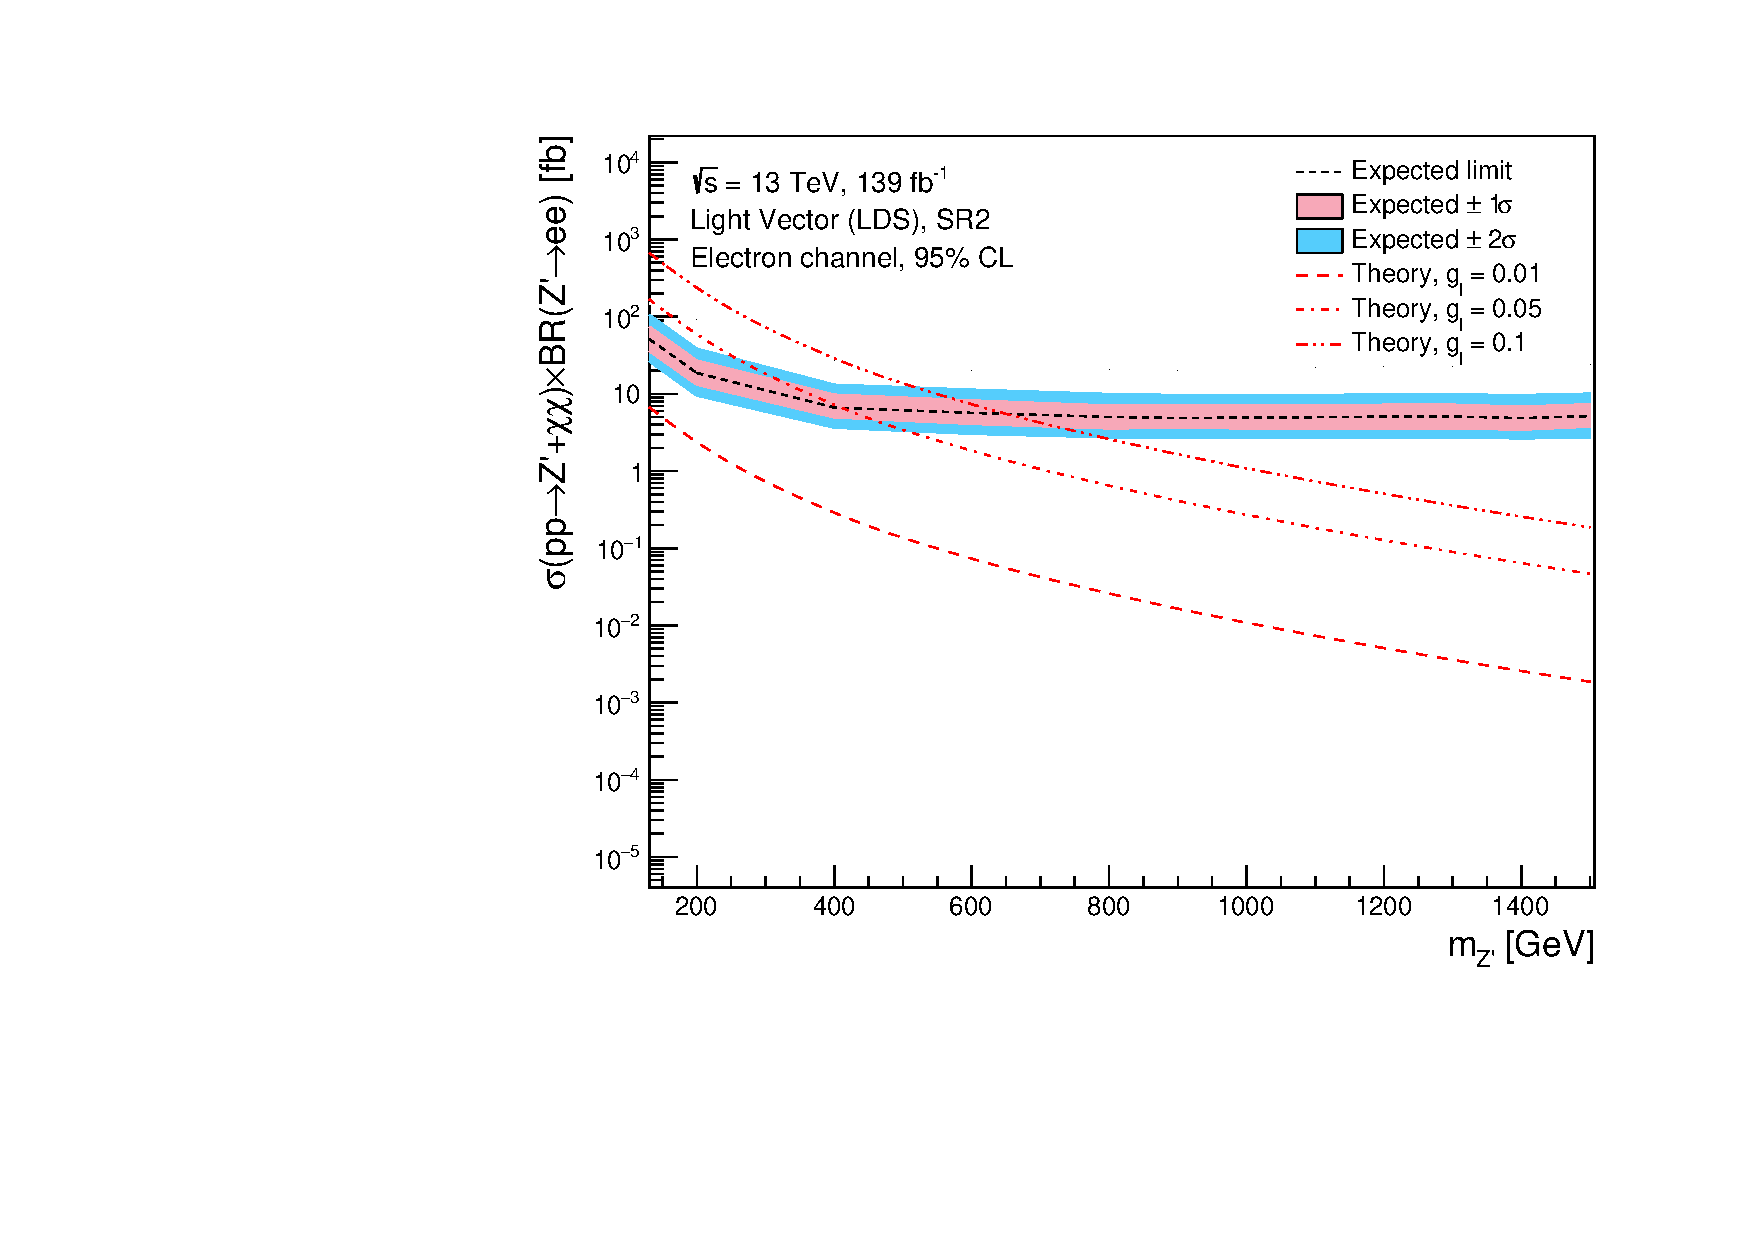
\includegraphics[width=1\textwidth]{Limits/Model_independent/100-150/LV_LDS/mass_exclusion_ee.pdf}
   \end{subfigure}
   \hfill
   \begin{subfigure}[b]{0.49\textwidth}
      \centering
      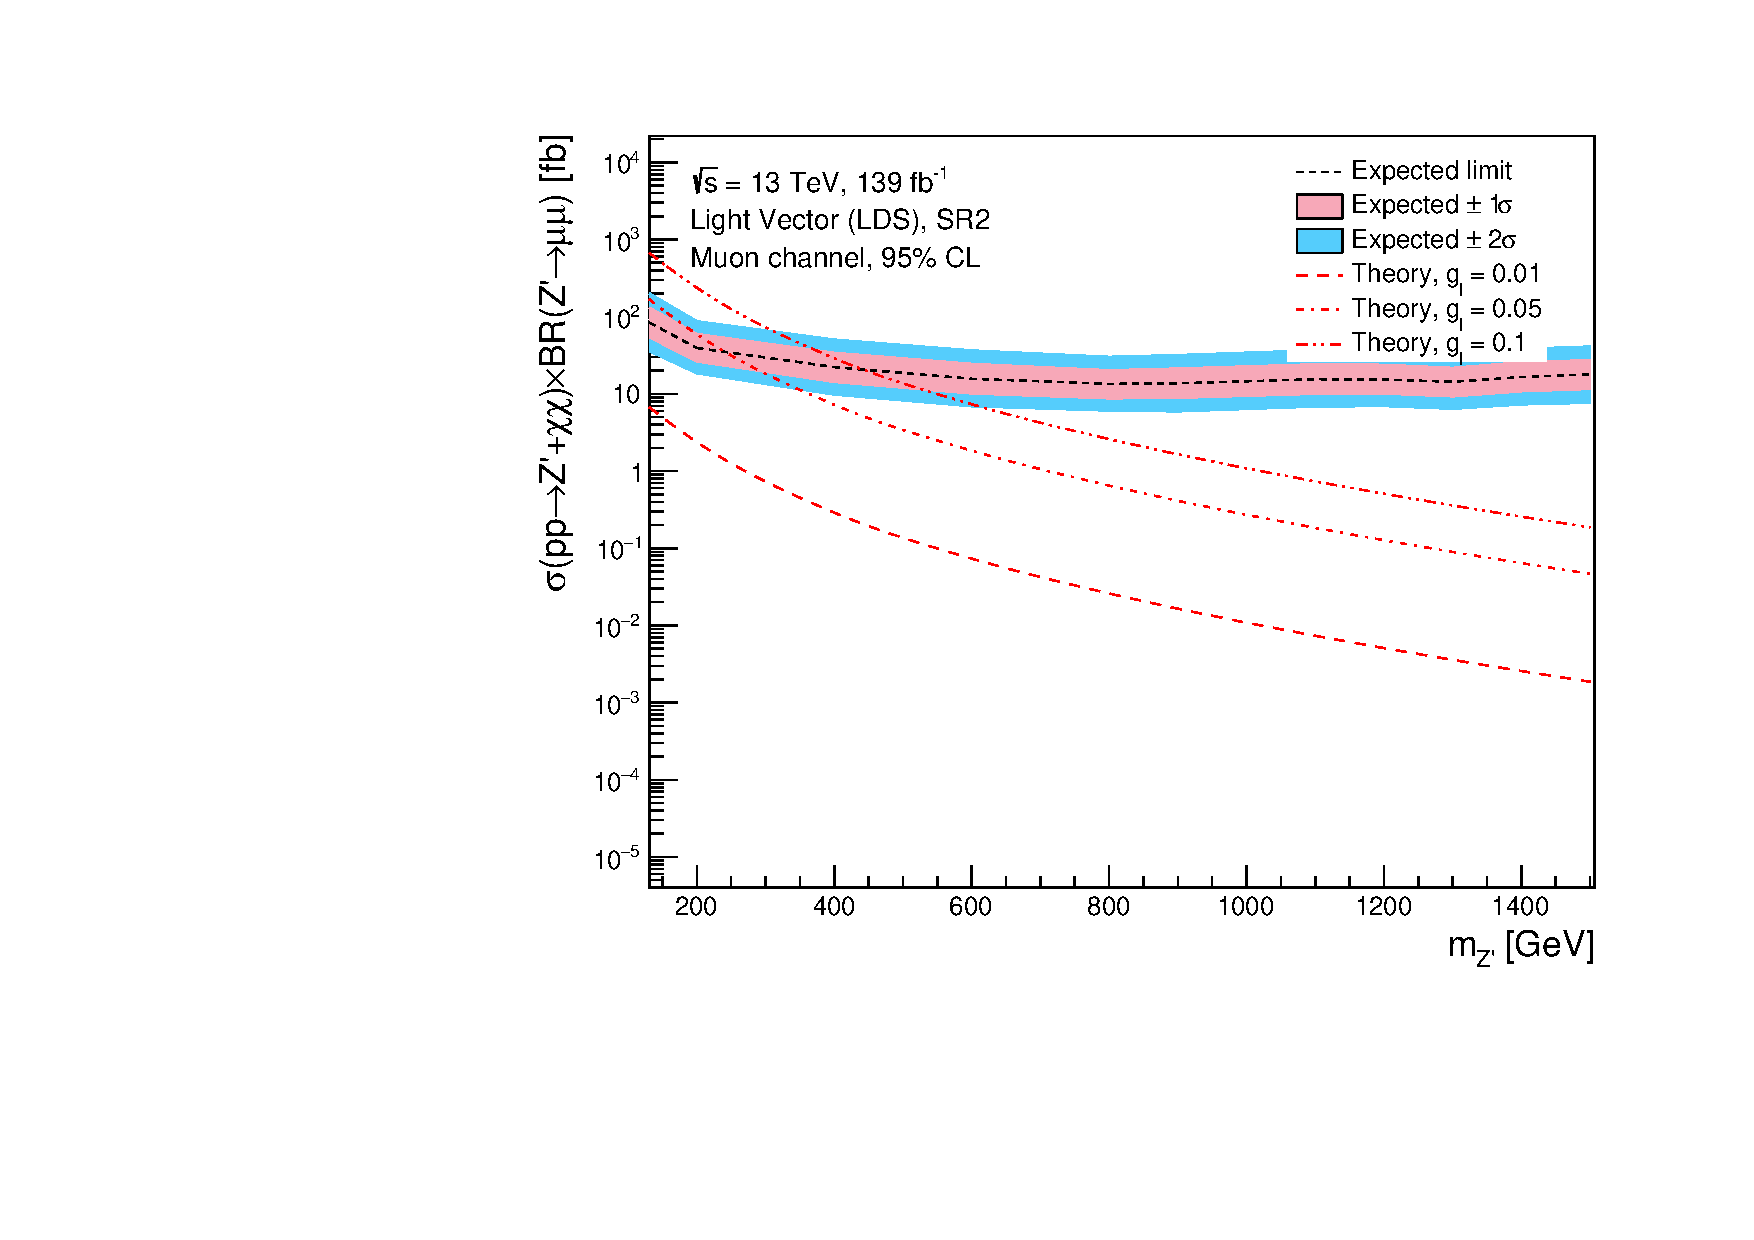
\includegraphics[width=1\textwidth]{Limits/Model_independent/100-150/LV_LDS/mass_exclusion_uu.pdf}
   \end{subfigure}
   \hfill
	\begin{subfigure}[b]{0.49\textwidth}
      \centering
      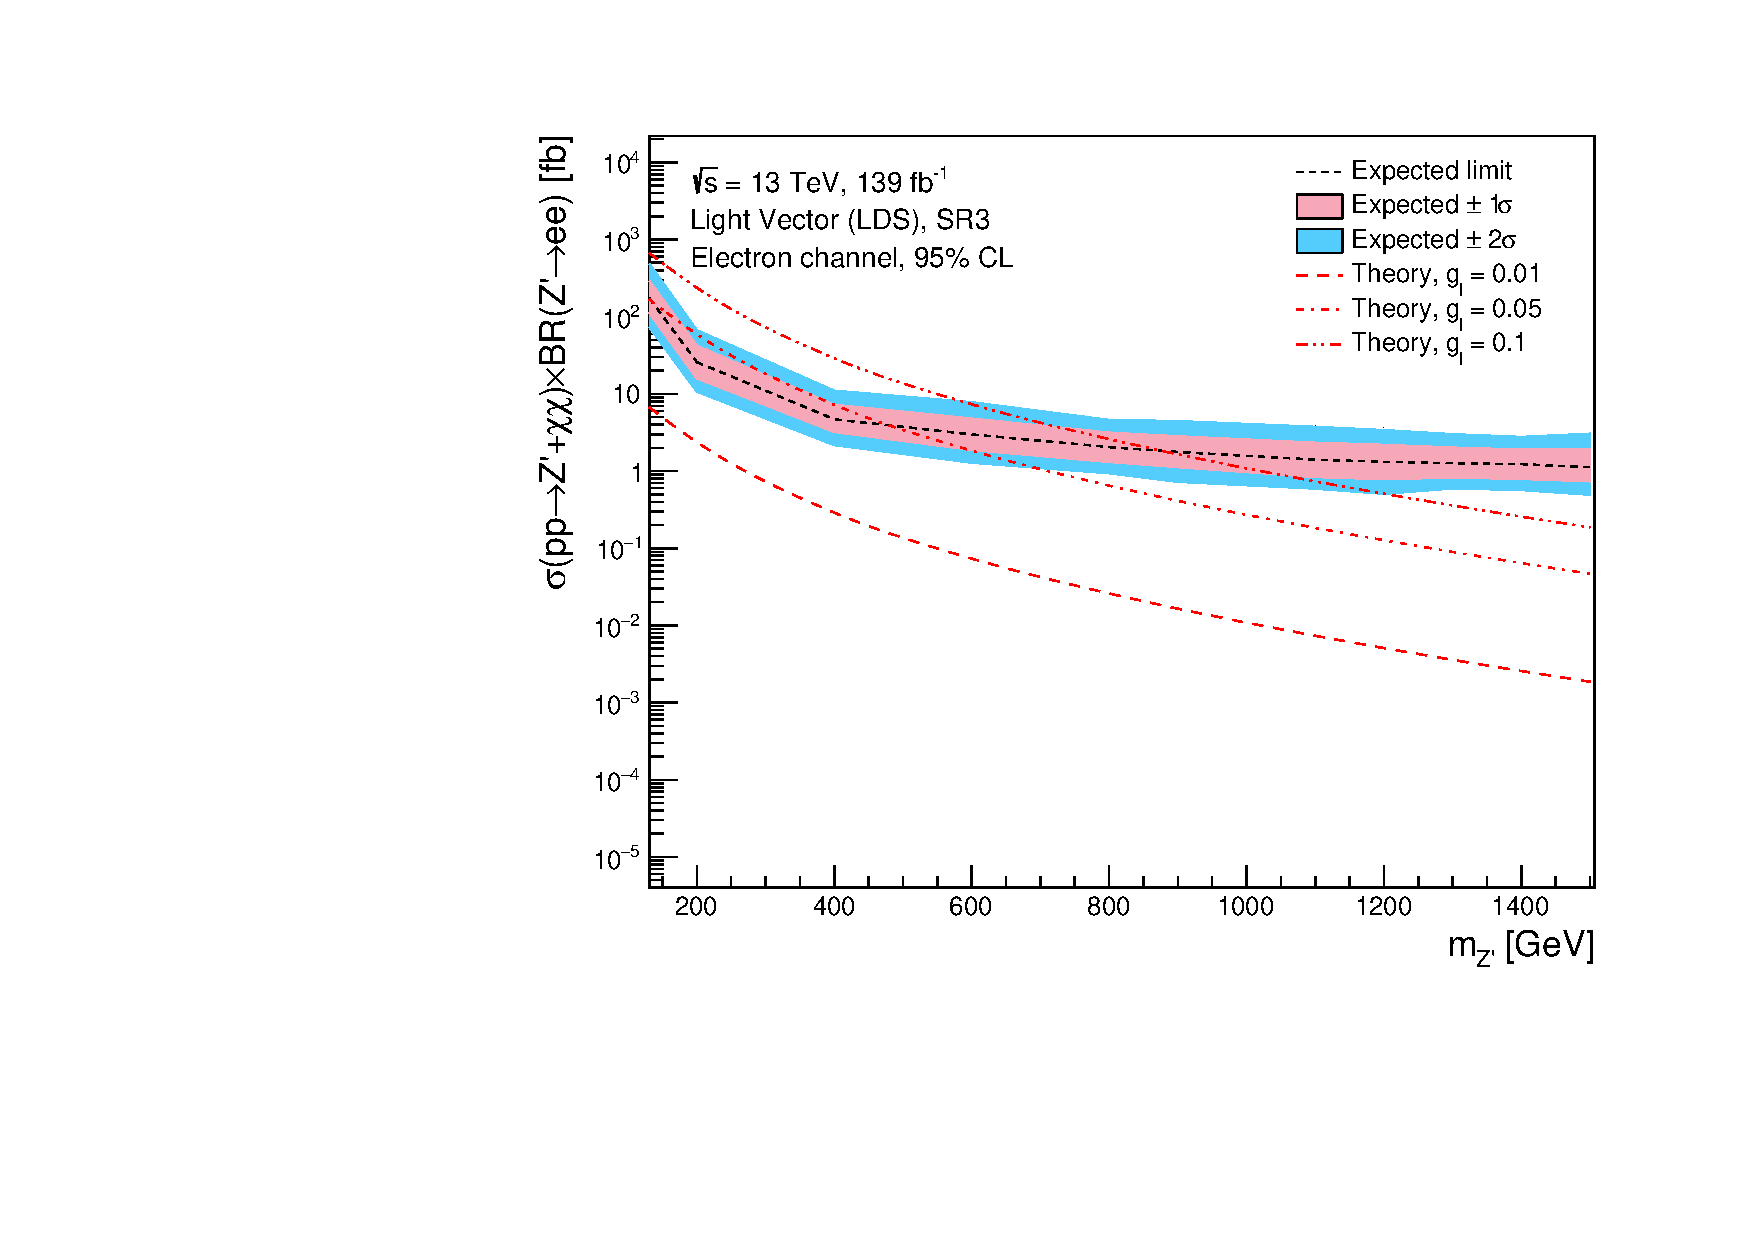
\includegraphics[width=1\textwidth]{Limits/Model_independent/150/LV_LDS/mass_exclusion_ee.pdf}
   \end{subfigure}
   \hfill
   \begin{subfigure}[b]{0.49\textwidth}
      \centering
      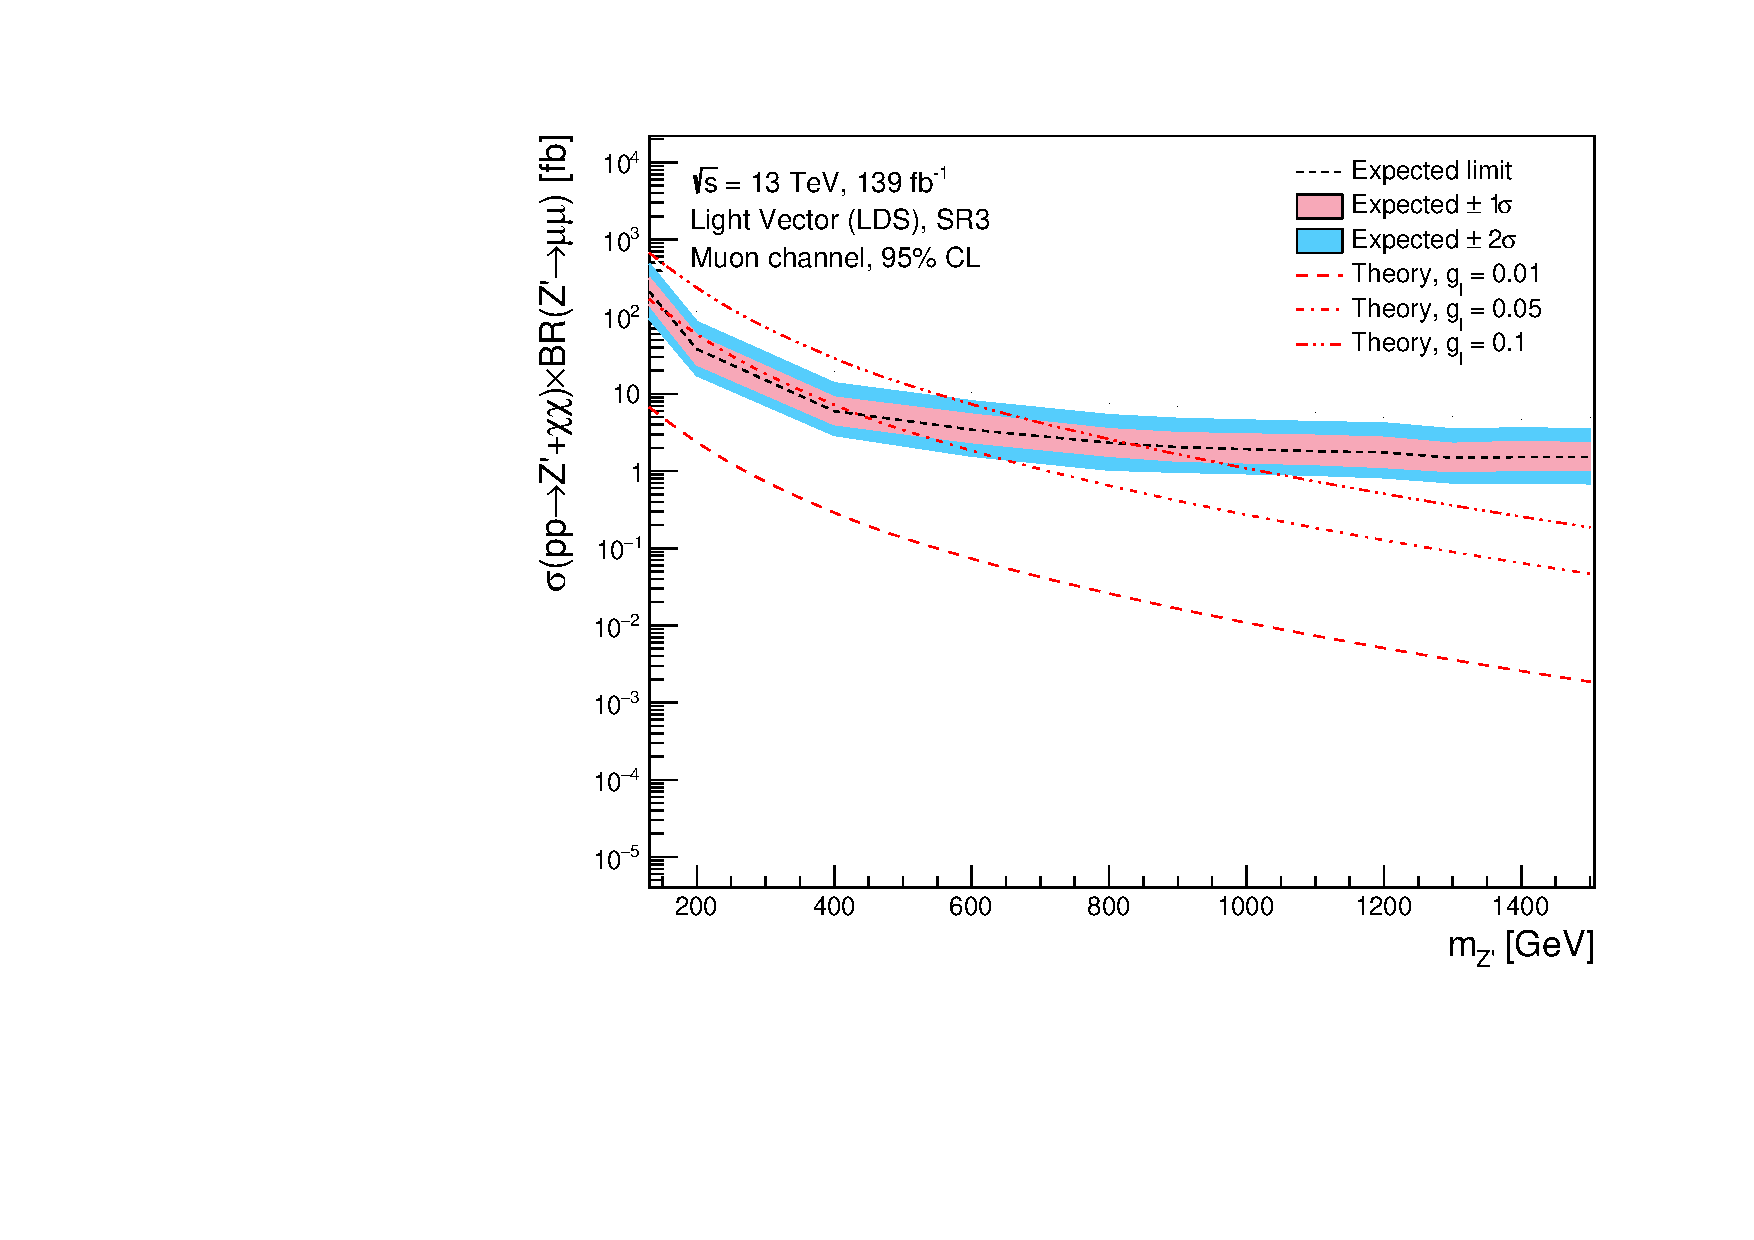
\includegraphics[width=1\textwidth]{Limits/Model_independent/150/LV_LDS/mass_exclusion_uu.pdf}
   \end{subfigure}
   \caption[Expected mass exclusion limits results for LV LDS model on $ee$ and $\mu\mu$ channel using the model independent approach]{Mass exclusion limits of $ee$ (left) and $\mu\mu$ (right) channel for Z' Light Vector Light Dark Sector model using the model independent approach. To remind what the SRs are: SR1 has $E_T^{miss}\in[50, 100]$ GeV, SR2 has $E_T^{miss}\in[100, 150]$ GeV, and SR3 has $E_T^{miss}>150$ GeV. The y-axis of both plots represents the cross-section times branching ratio of the process we are studying. The x-axis is the mass of the $Z'$ boson. We did not interpolate between the available masses we had simulated, 
   and have rather just connected the values calculated for each mass point by connecting the points. The dashed black line is the expected 95\% CL limit with a 1$\sigma$ and 2$\sigma$ variance. 
   The different red dashed lines represent the theoretical cross-section times branching ratio of the process when varying the value of the lepton coupling $g_l$ between the leptons and the $Z'$ boson. The simulated events in this thesis utilized the value $g_l=$ 0.01, we include the cross-section times branching ratio when increasing this coupling to 0.05 and 0.1 to see how the exclusions change.  }\label{fig:LV_LDS_me_SRS}
\end{figure}


\clearpage
\section{Effective Field Theory Heavy Dark Sector}
\begin{figure}[!ht]
	\centering
   \begin{subfigure}[b]{0.49\textwidth}
      \centering
      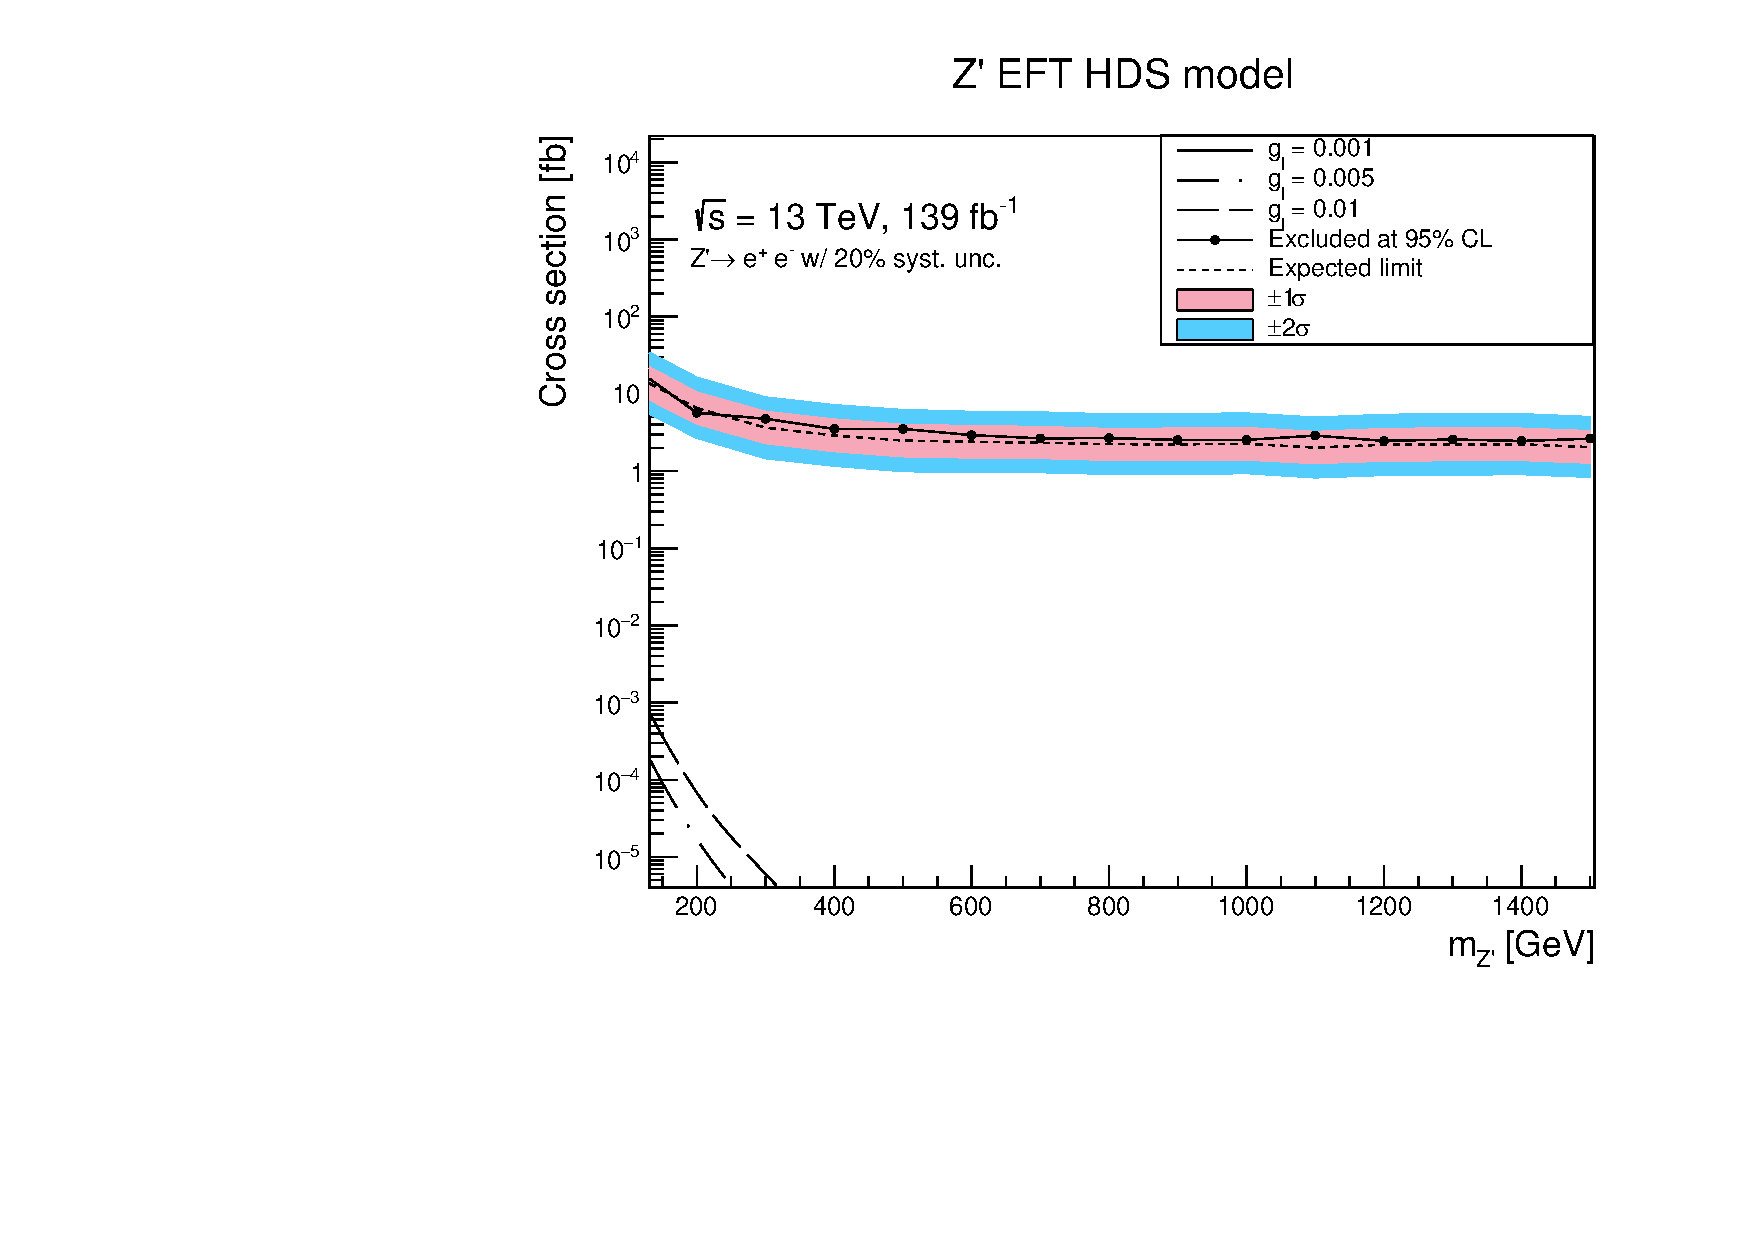
\includegraphics[width=1\textwidth]{Limits/EFT_HDS/mass_exclusion_ee.pdf}
      \end{subfigure}
   \hfill
   \begin{subfigure}[b]{0.49\textwidth}
      \centering
      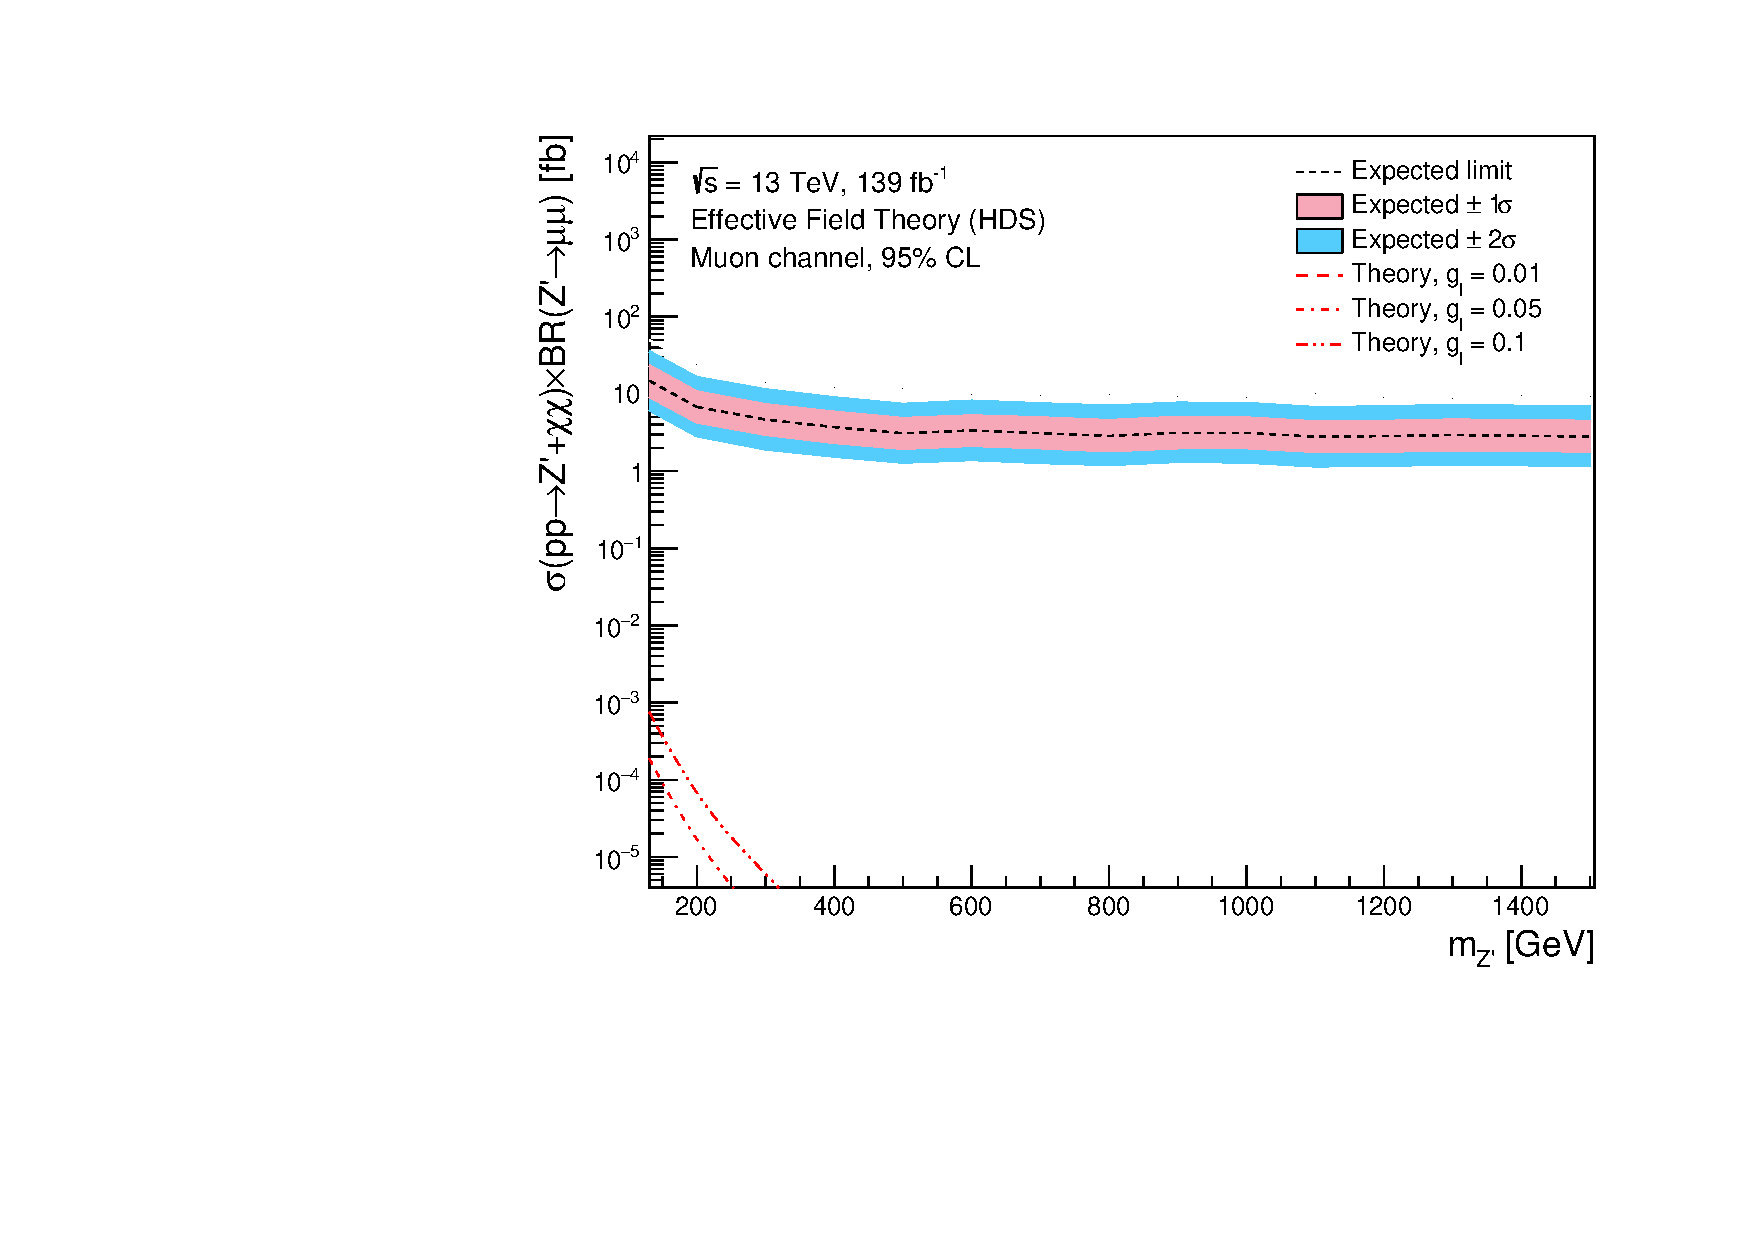
\includegraphics[width=1\textwidth]{Limits/EFT_HDS/mass_exclusion_uu.pdf}
      \end{subfigure}
   \caption[Expected mass exclusion limits of $ee$ and $\mu\mu$ channel for all Z' EFT HDS model using the model dependent approach]{Mass exclusion limits of $ee$ (left) and $\mu\mu$ (right) channel for Z' EFT Heavy Dark Sector model using the model dependent approach. The y-axis of both plots represents the cross-section times branching ratio of the process we are studying. The x-axis is the mass of the $Z'$ boson. We did not interpolate between the available masses we had simulated, 
   and have rather just connected the values calculated for each mass point by connecting the points. The dashed black line is the expected 95\% CL limit with a 1$\sigma$ and 2$\sigma$ variance. 
   The different red dashed lines represent the theoretical cross-section times branching ratio of the process when varying the value of the lepton coupling $g_l$ between the leptons and the $Z'$ boson. The simulated events in this thesis utilized the value $g_l=$ 0.01, we include the cross-section times branching ratio when increasing this coupling to 0.05 and 0.1 to see how the exclusions change.  }\label{fig:EFT_HDS_exclusion_ee_uu}
\end{figure}
\begin{figure}[!ht]
	\centering
	\begin{subfigure}[b]{0.49\textwidth}
      \centering
      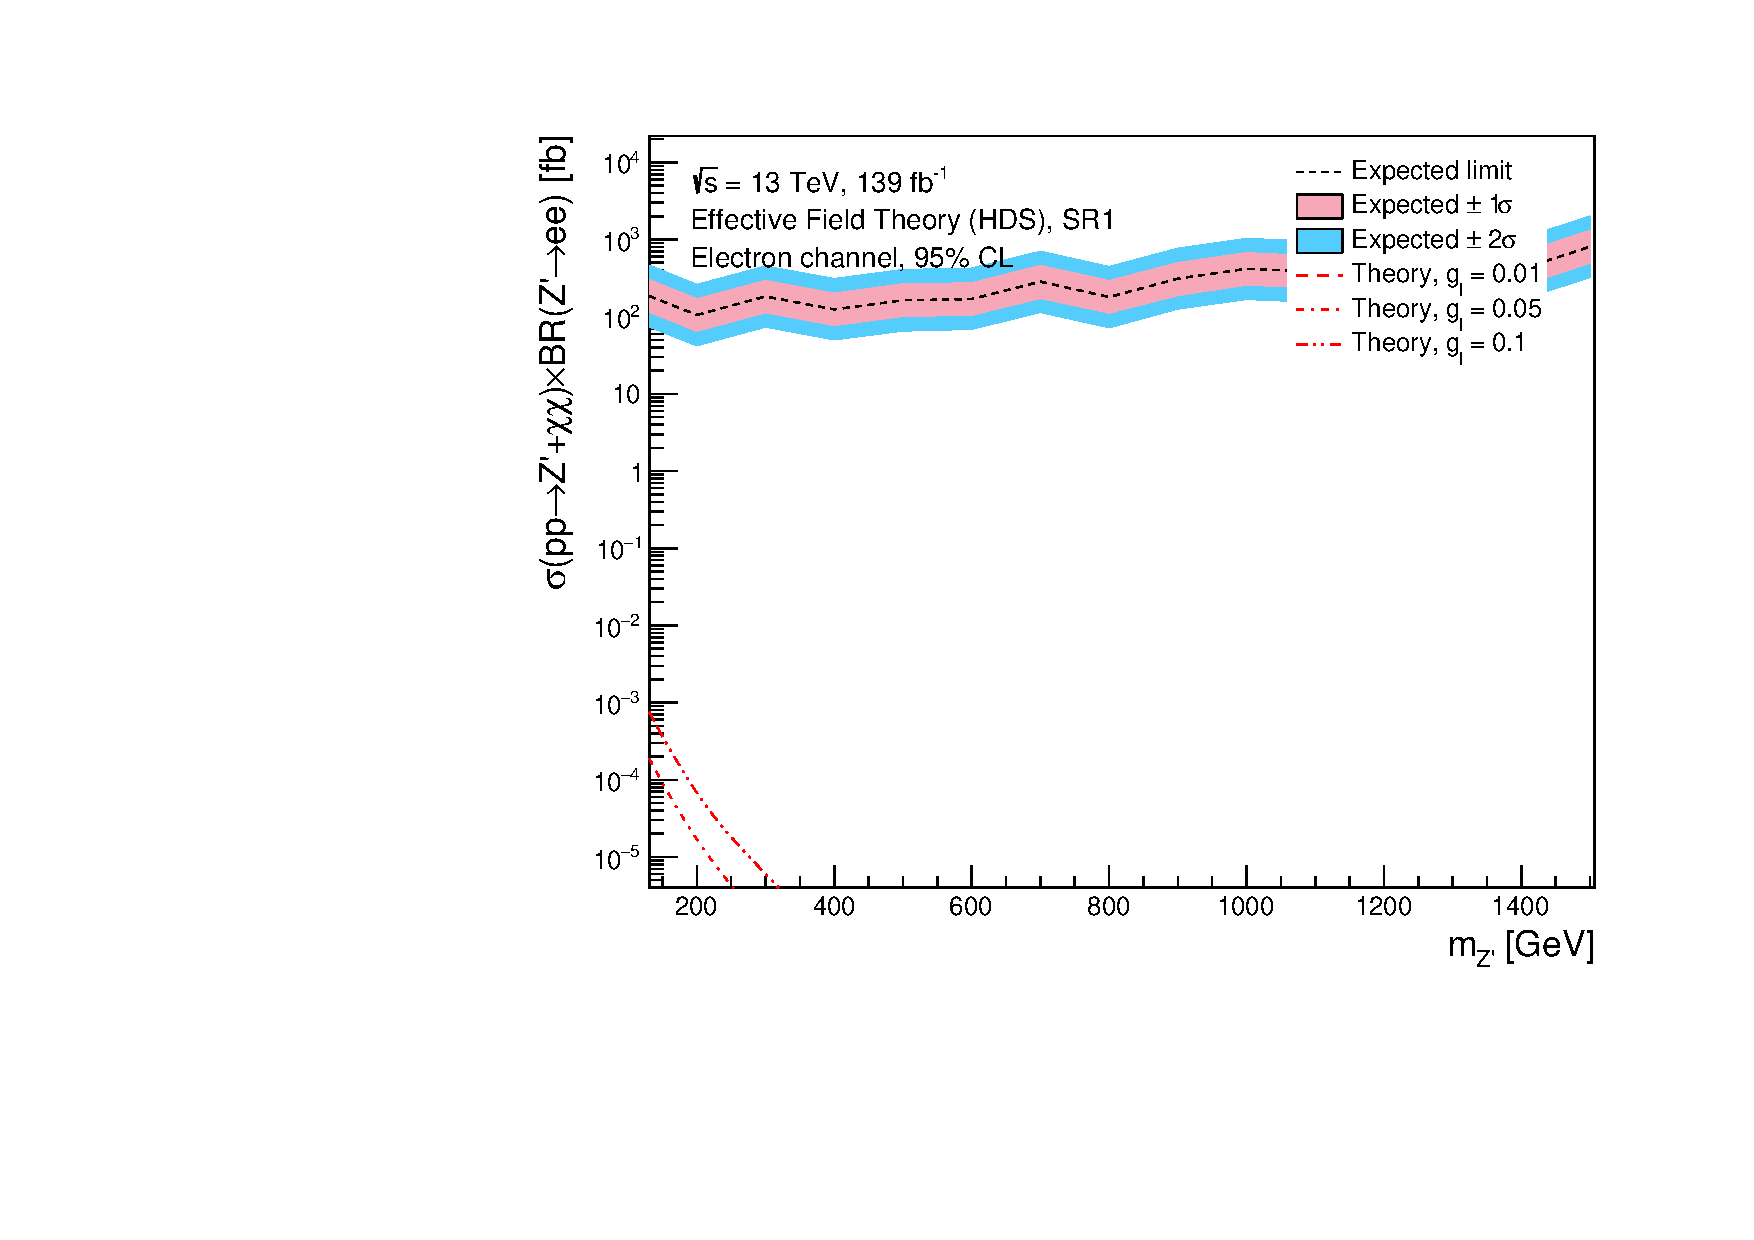
\includegraphics[width=1\textwidth]{Limits/Model_independent/50-100/EFT_HDS/mass_exclusion_ee.pdf}
   \end{subfigure}
   \hfill
   \begin{subfigure}[b]{0.49\textwidth}
      \centering
      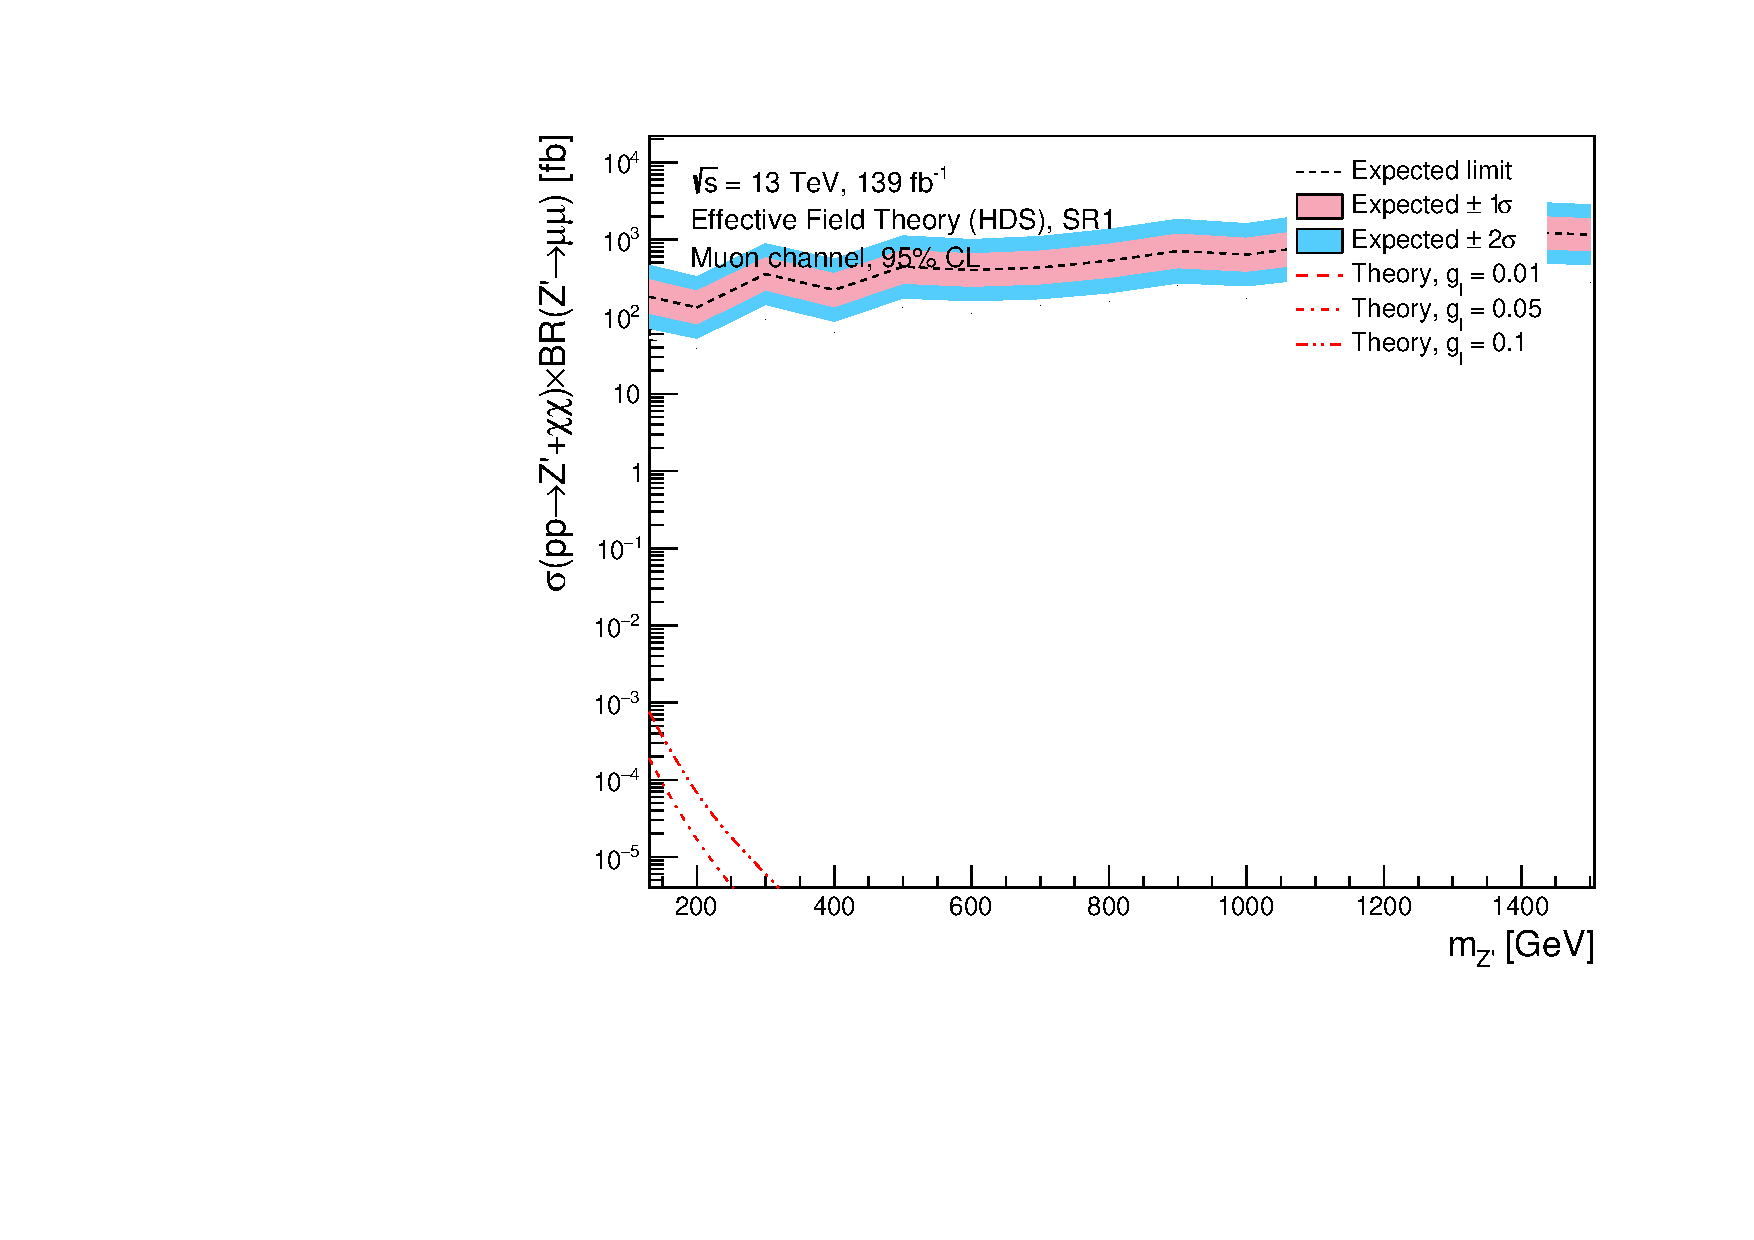
\includegraphics[width=1\textwidth]{Limits/Model_independent/50-100/EFT_HDS/mass_exclusion_uu.pdf}
   \end{subfigure}
   \hfill
   \begin{subfigure}[b]{0.49\textwidth}
      \centering
      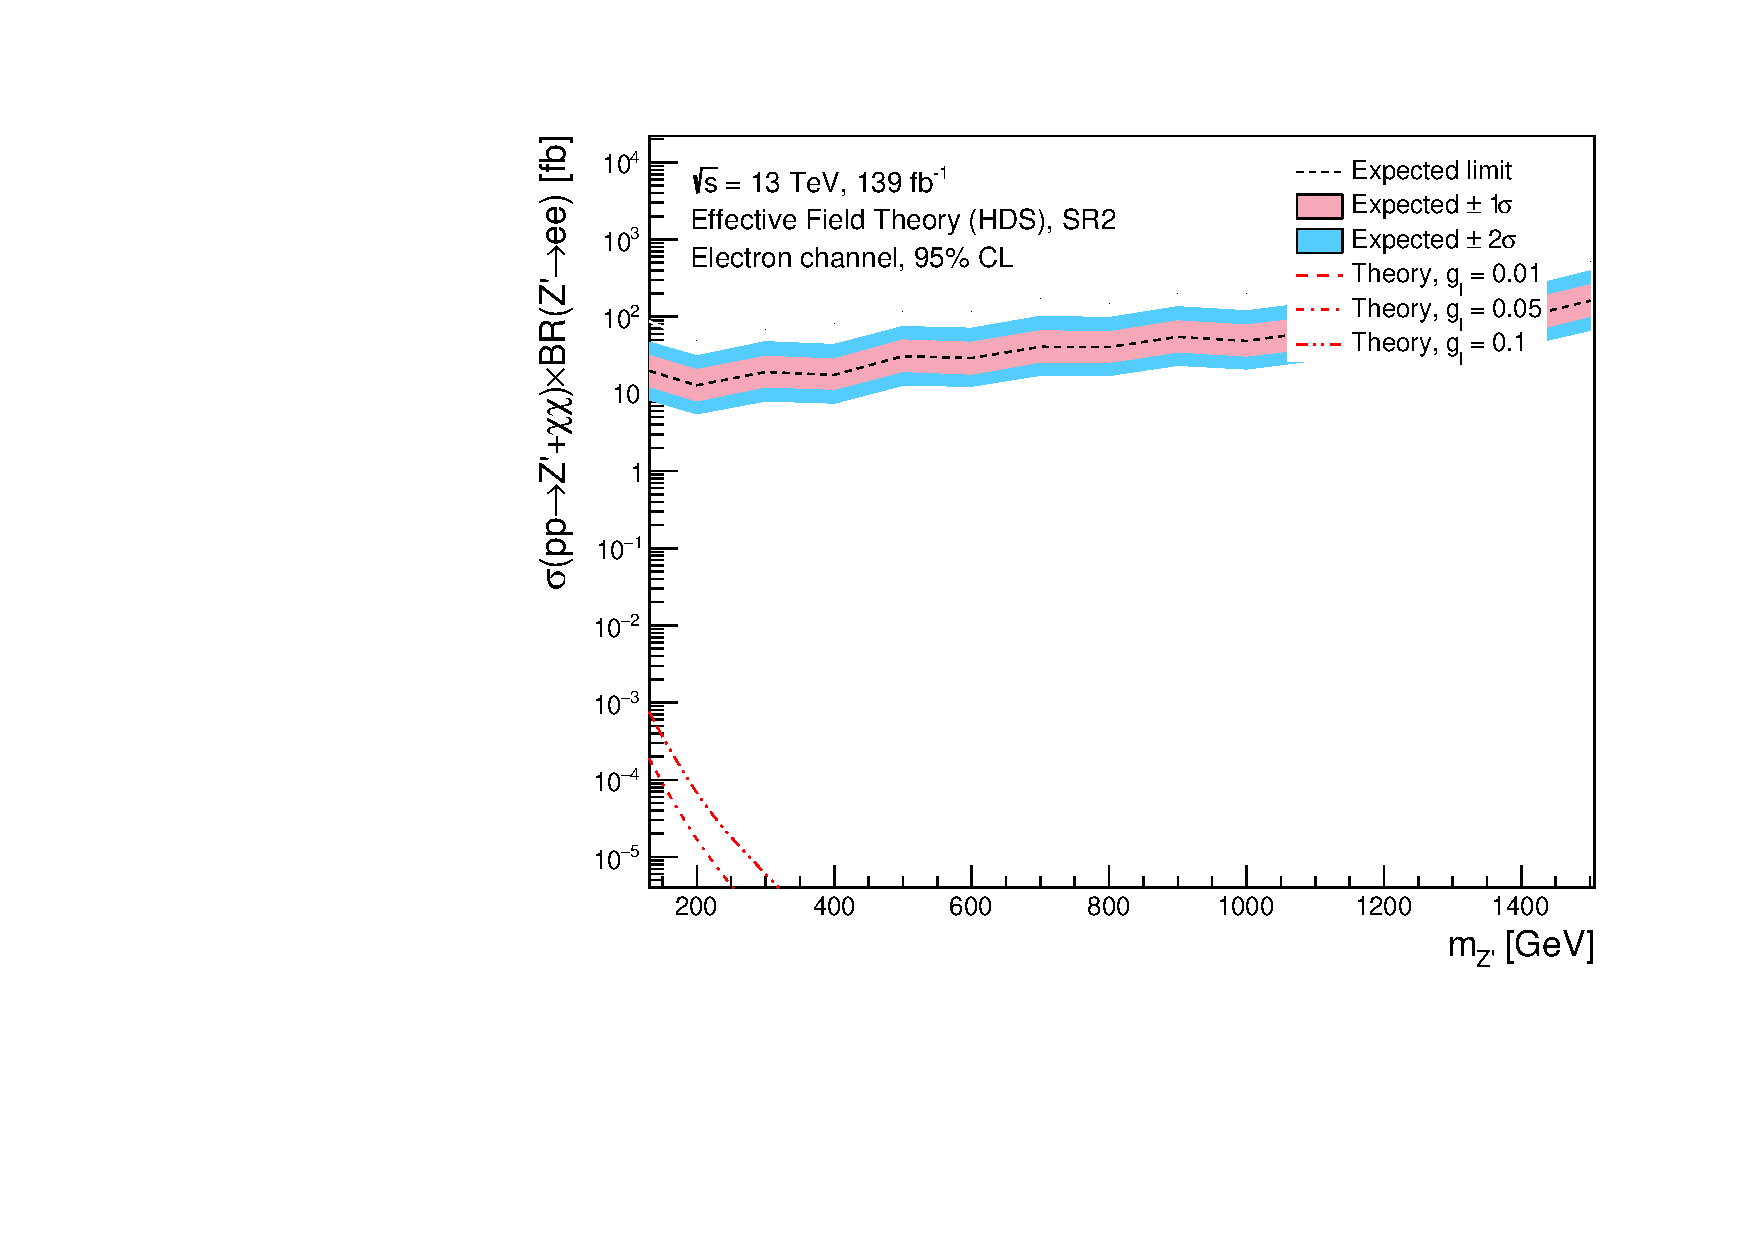
\includegraphics[width=1\textwidth]{Limits/Model_independent/100-150/EFT_HDS/mass_exclusion_ee.pdf}
   \end{subfigure}
   \hfill
   \begin{subfigure}[b]{0.49\textwidth}
      \centering
      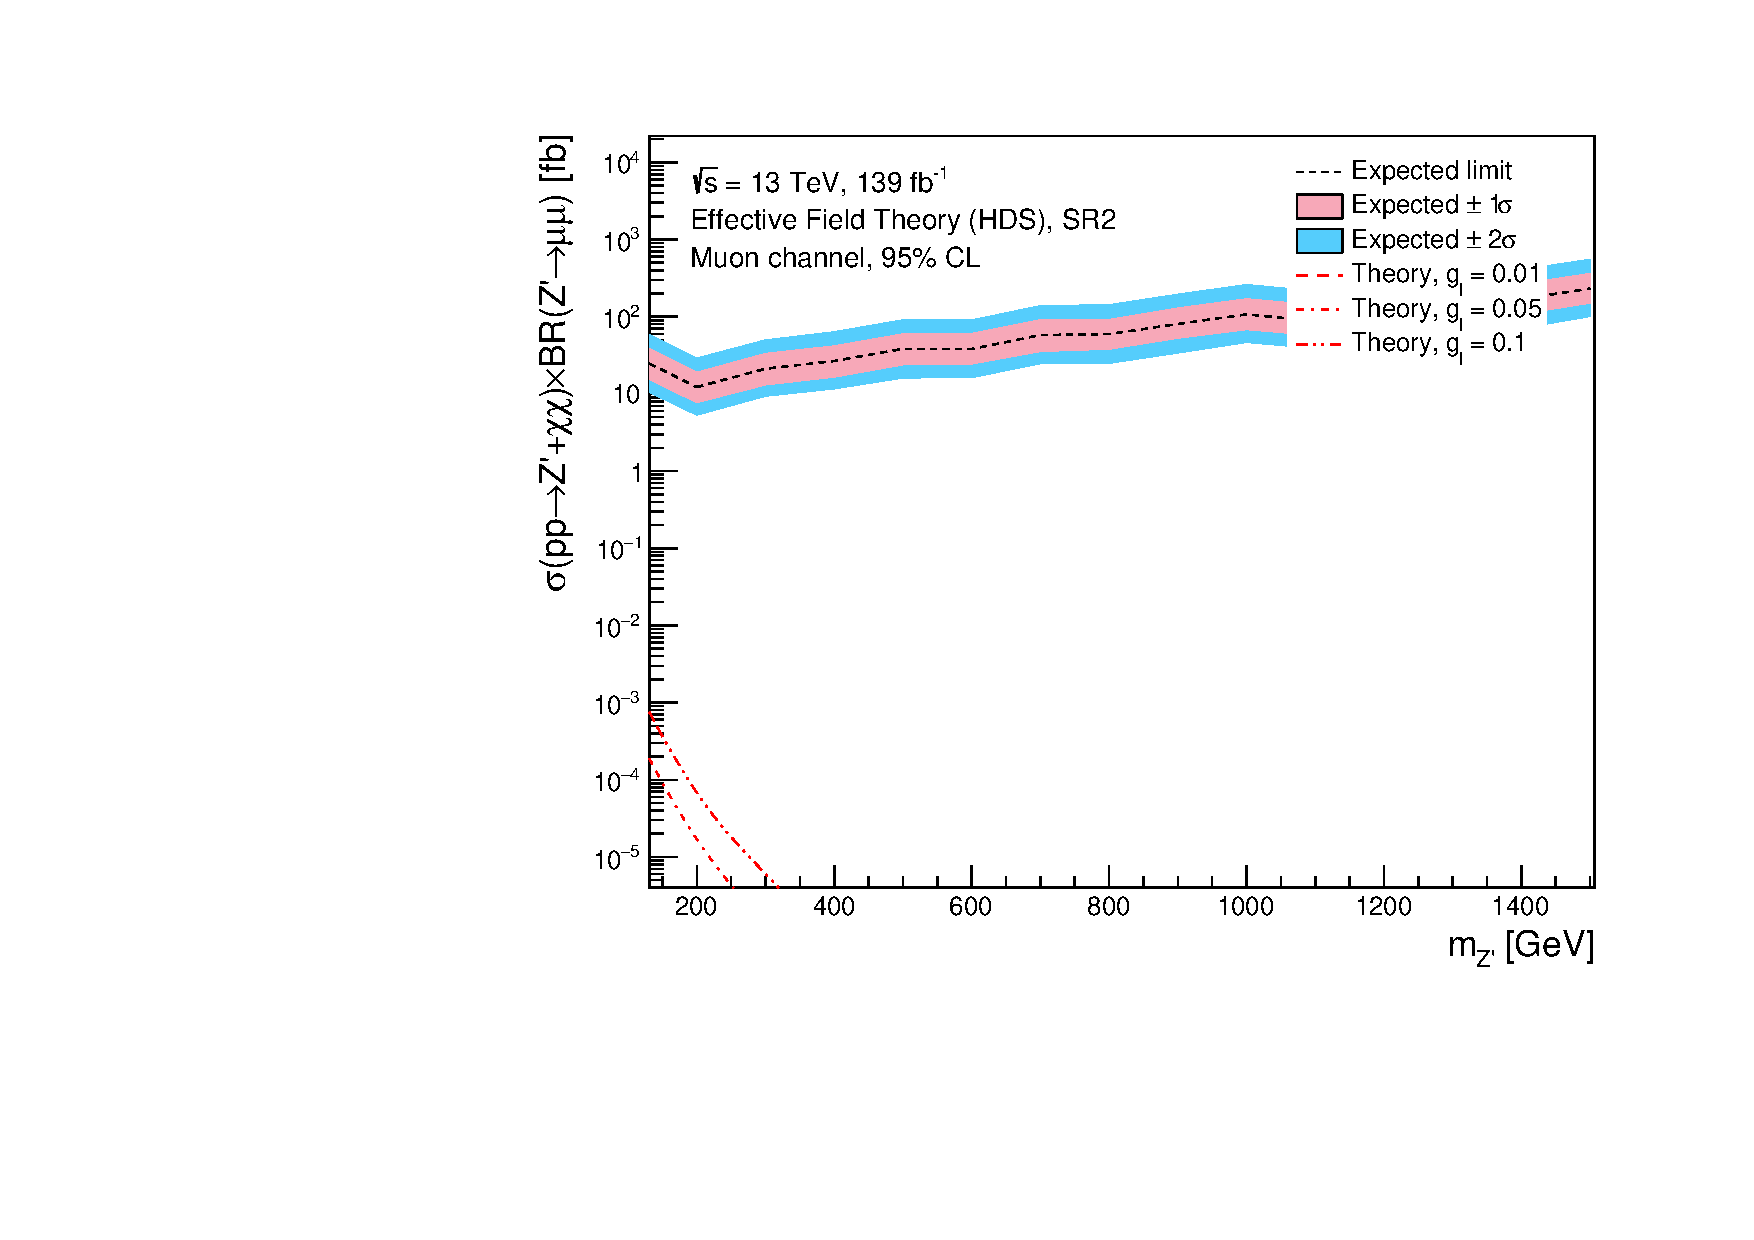
\includegraphics[width=1\textwidth]{Limits/Model_independent/100-150/EFT_HDS/mass_exclusion_uu.pdf}
   \end{subfigure}
   \hfill
	\begin{subfigure}[b]{0.49\textwidth}
      \centering
      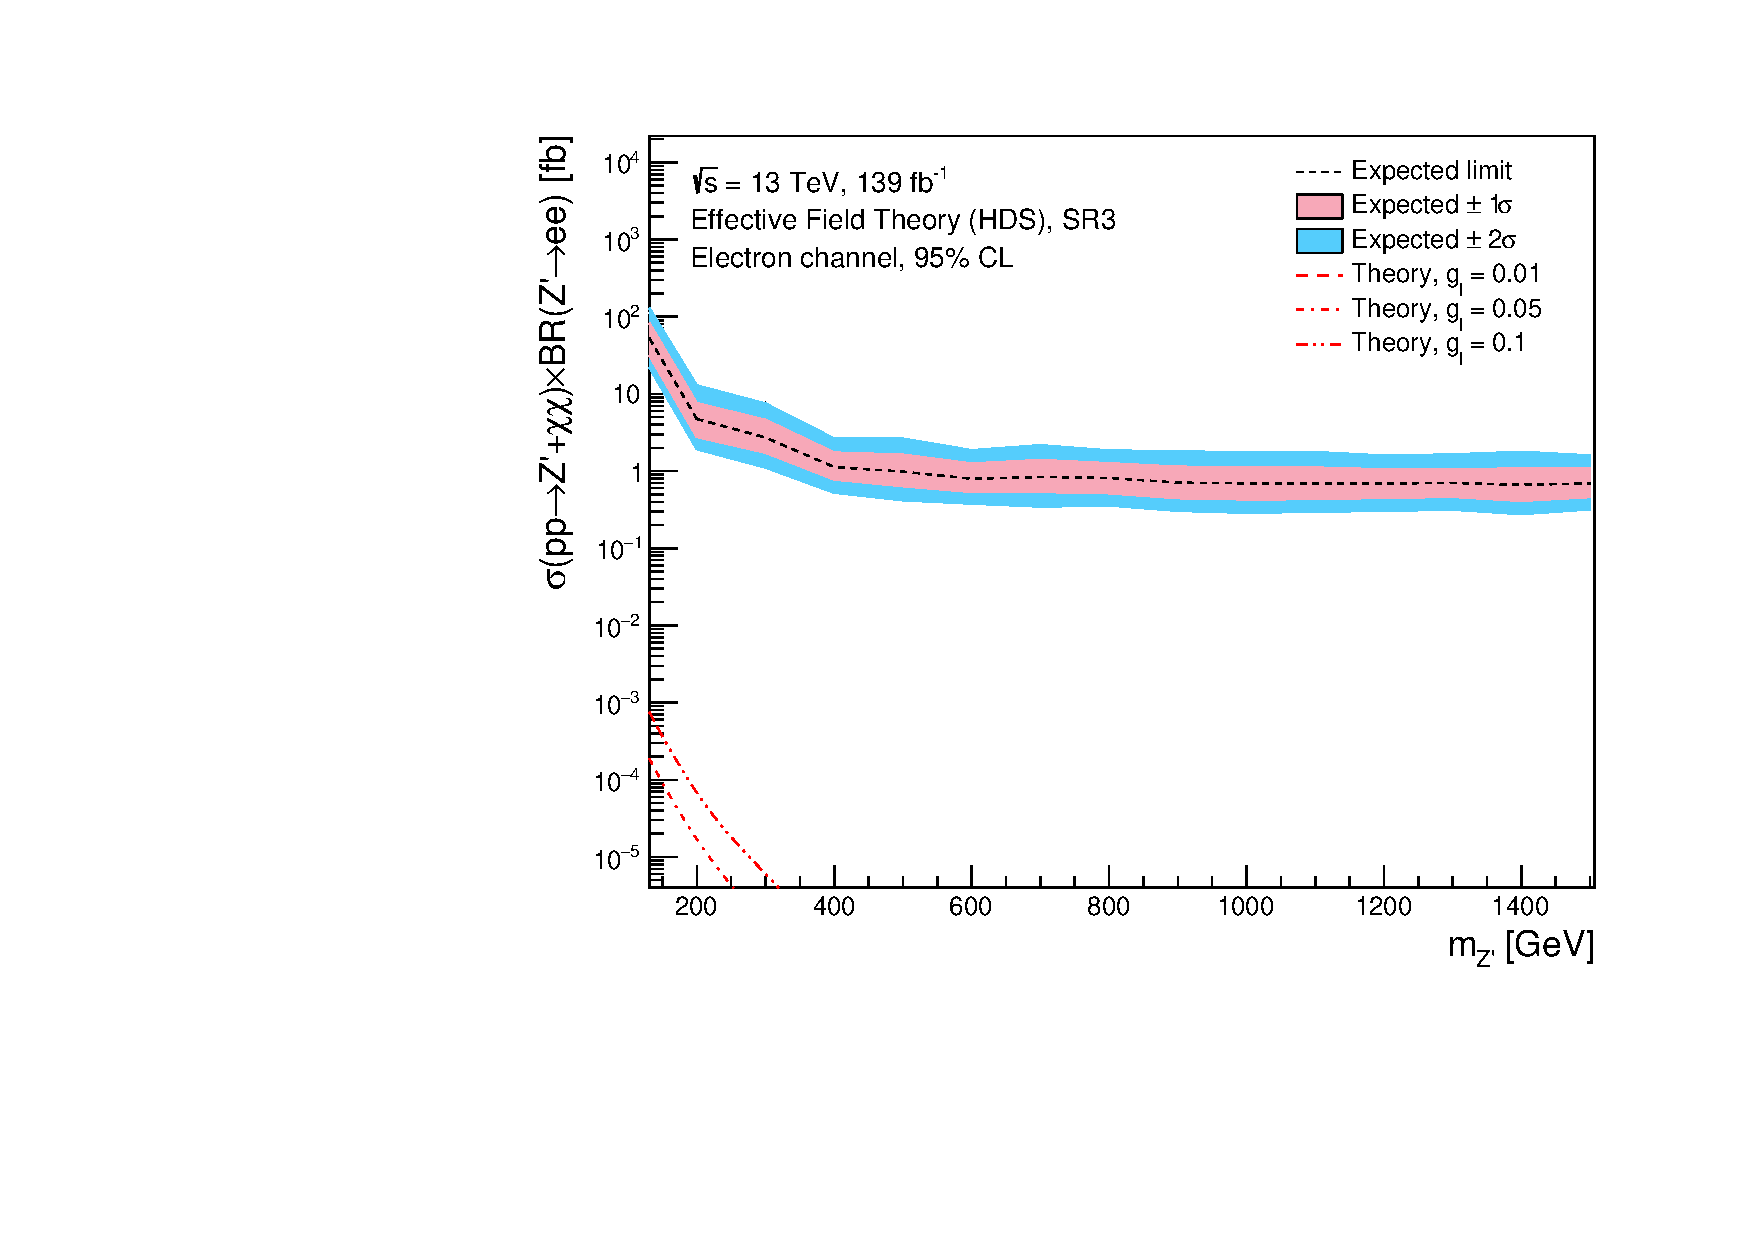
\includegraphics[width=1\textwidth]{Limits/Model_independent/150/EFT_HDS/mass_exclusion_ee.pdf}
   \end{subfigure}
   \hfill
   \begin{subfigure}[b]{0.49\textwidth}
      \centering
      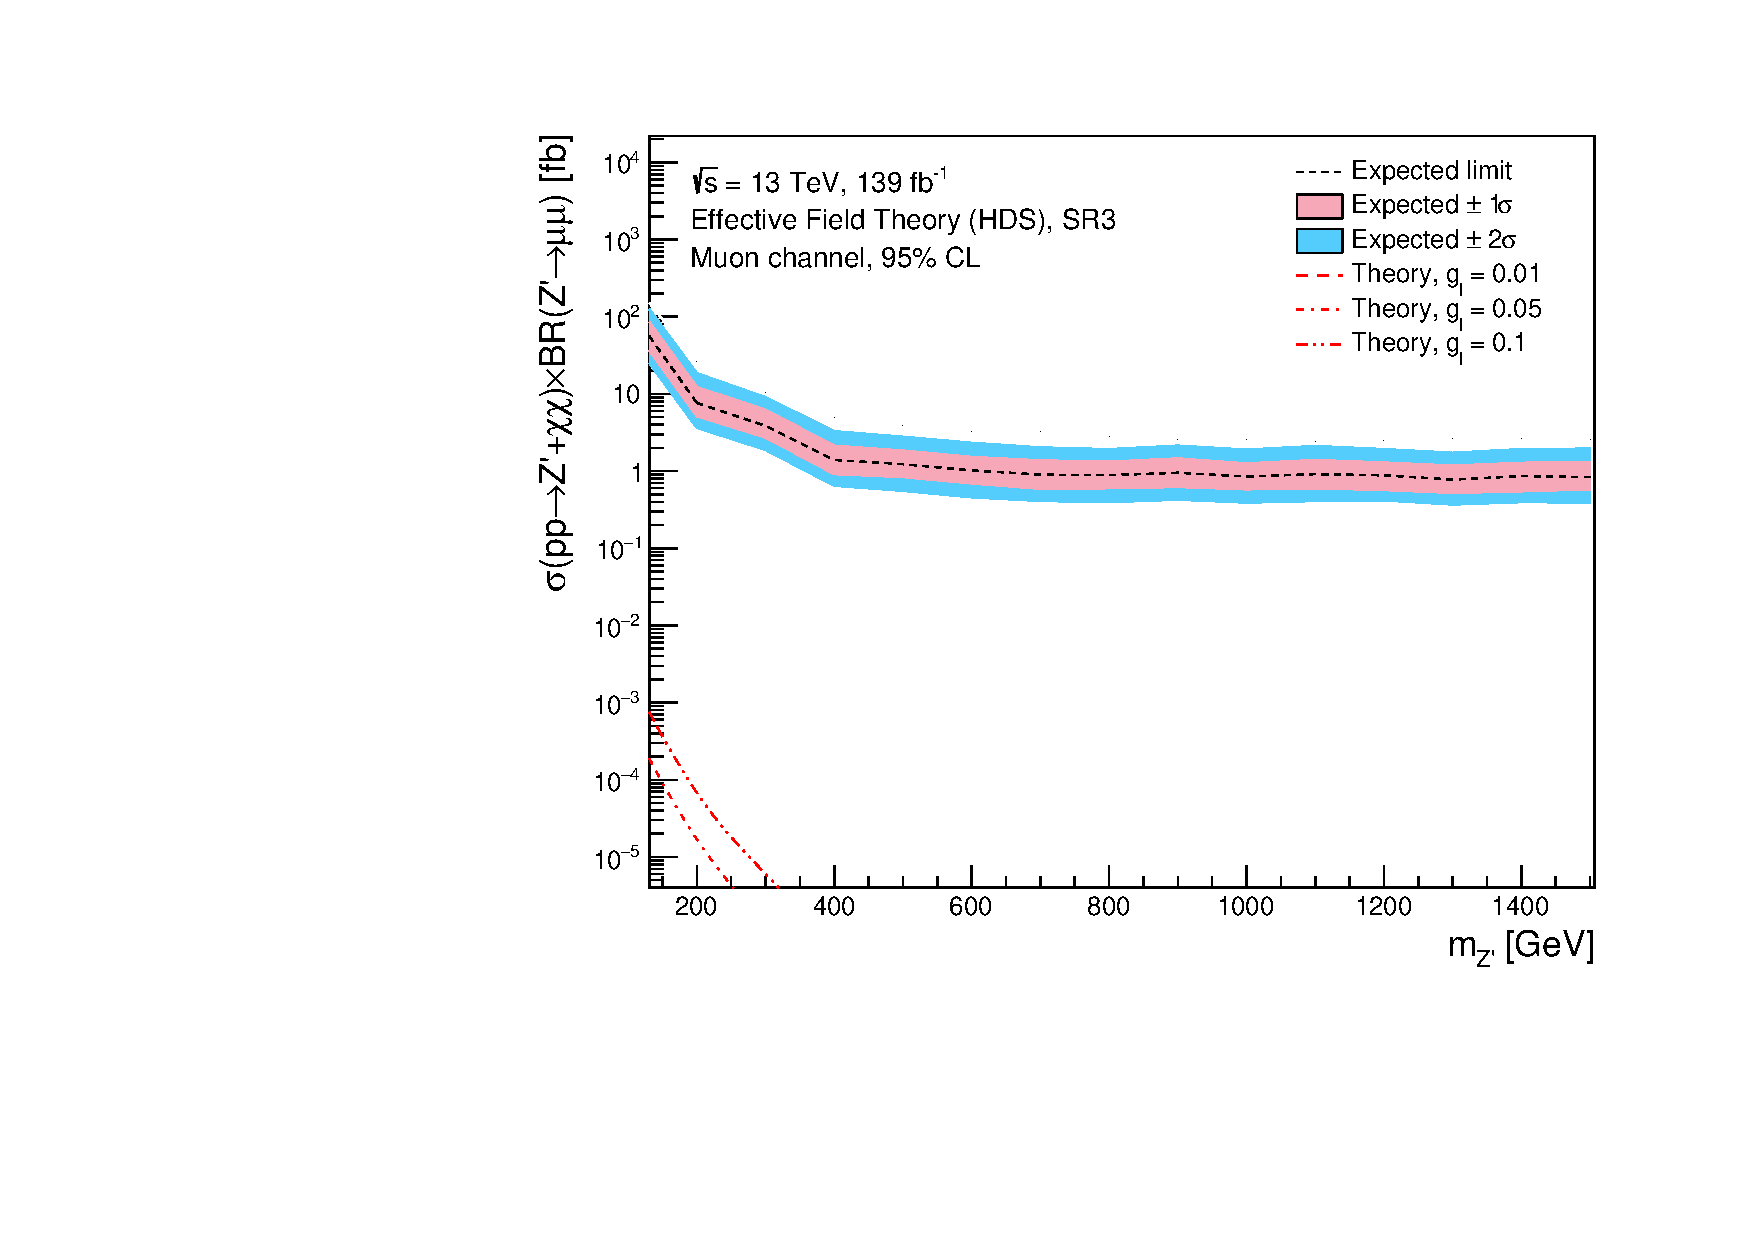
\includegraphics[width=1\textwidth]{Limits/Model_independent/150/EFT_HDS/mass_exclusion_uu.pdf}
   \end{subfigure}
   \caption[Expected mass exclusion limits results for EFT HDS model on $ee$ and $\mu\mu$ channel using the model independent approach]{Mass exclusion limits of $ee$ (left) and $\mu\mu$ (right) channel for Z' EFT Heavy Dark Sector model using the model independent approach. To remind what the SRs are: SR1 has $E_T^{miss}\in[50, 100]$ GeV, SR2 has $E_T^{miss}\in[100, 150]$ GeV, and SR3 has $E_T^{miss}>150$ GeV. The y-axis of both plots represents the cross-section times branching ratio of the process we are studying. The x-axis is the mass of the $Z'$ boson. We did not interpolate between the available masses we had simulated, 
   and have rather just connected the values calculated for each mass point by connecting the points. The dashed black line is the expected 95\% CL limit with a 1$\sigma$ and 2$\sigma$ variance. 
   The different red dashed lines represent the theoretical cross-section times branching ratio of the process when varying the value of the lepton coupling $g_l$ between the leptons and the $Z'$ boson. The simulated events in this thesis utilized the value $g_l=$ 0.01, we include the cross-section times branching ratio when increasing this coupling to 0.05 and 0.1 to see how the exclusions change.  }\label{fig:EFT_HDS_me_SRS}
\end{figure}







\clearpage
\section{Effective Field Theory Light Dark Sector}
\begin{figure}[!ht]
	\centering
   \begin{subfigure}[b]{0.49\textwidth}
      \centering
      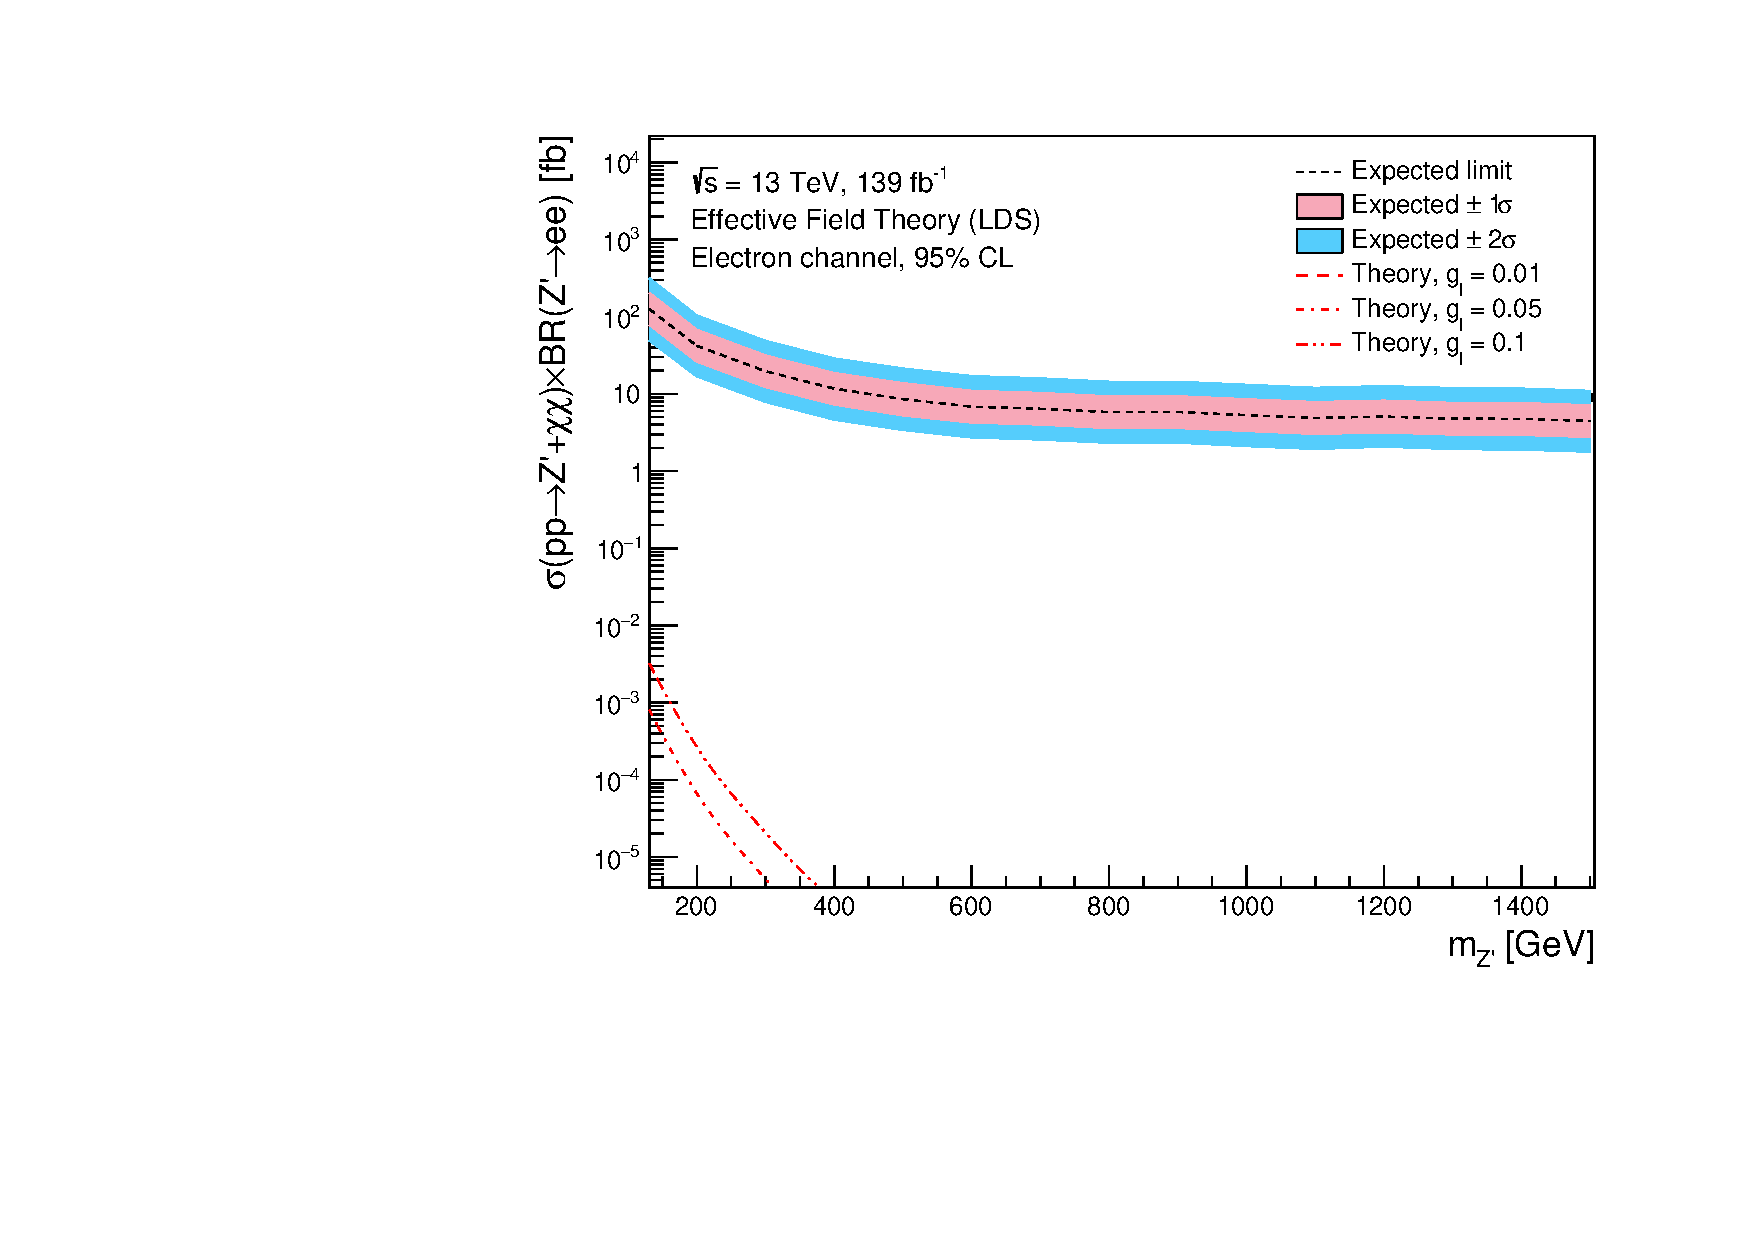
\includegraphics[width=1\textwidth]{Limits/EFT_LDS/mass_exclusion_ee.pdf}
      \end{subfigure}
   \hfill
   \begin{subfigure}[b]{0.49\textwidth}
      \centering
      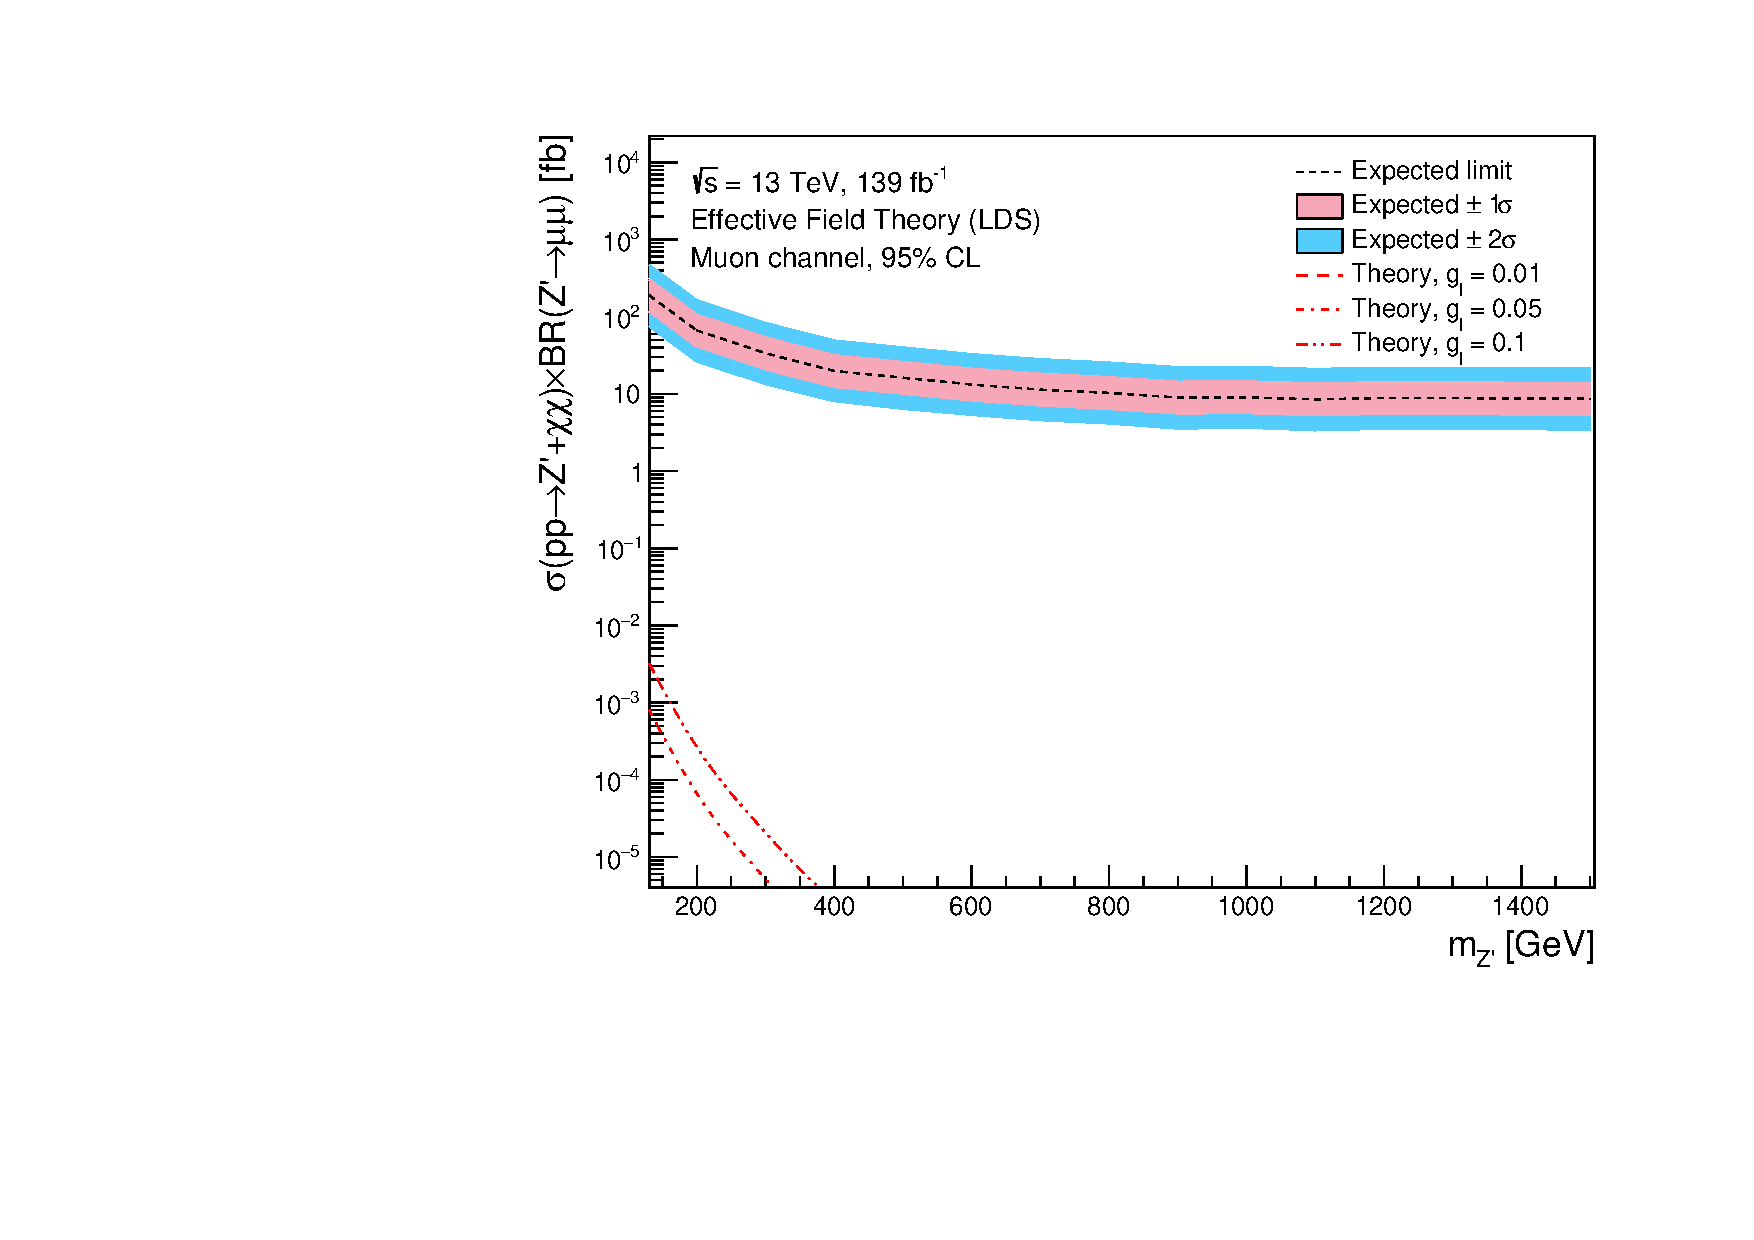
\includegraphics[width=1\textwidth]{Limits/EFT_LDS/mass_exclusion_uu.pdf}
      \end{subfigure}
   \caption[Expected mass exclusion limits of $ee$ and $\mu\mu$ channel for Z' EFT LDS model using the model dependent approach]{Mass exclusion limits of $ee$ (left) and $\mu\mu$ (right) channel for Z' EFT Light Dark Sector model using the model dependent approach. The y-axis of both plots represents the cross-section times branching ratio of the process we are studying. The x-axis is the mass of the $Z'$ boson. We did not interpolate between the available masses we had simulated, 
   and have rather just connected the values calculated for each mass point by connecting the points. The dashed black line is the expected 95\% CL limit with a 1$\sigma$ and 2$\sigma$ variance. 
   The different red dashed lines represent the theoretical cross-section times branching ratio of the process when varying the value of the lepton coupling $g_l$ between the leptons and the $Z'$ boson. The simulated events in this thesis utilized the value $g_l=$ 0.01, we include the cross-section times branching ratio when increasing this coupling to 0.05 and 0.1 to see how the exclusions change.  }
\end{figure}

\begin{figure}[!ht]
	\centering
	\begin{subfigure}[b]{0.49\textwidth}
      \centering
      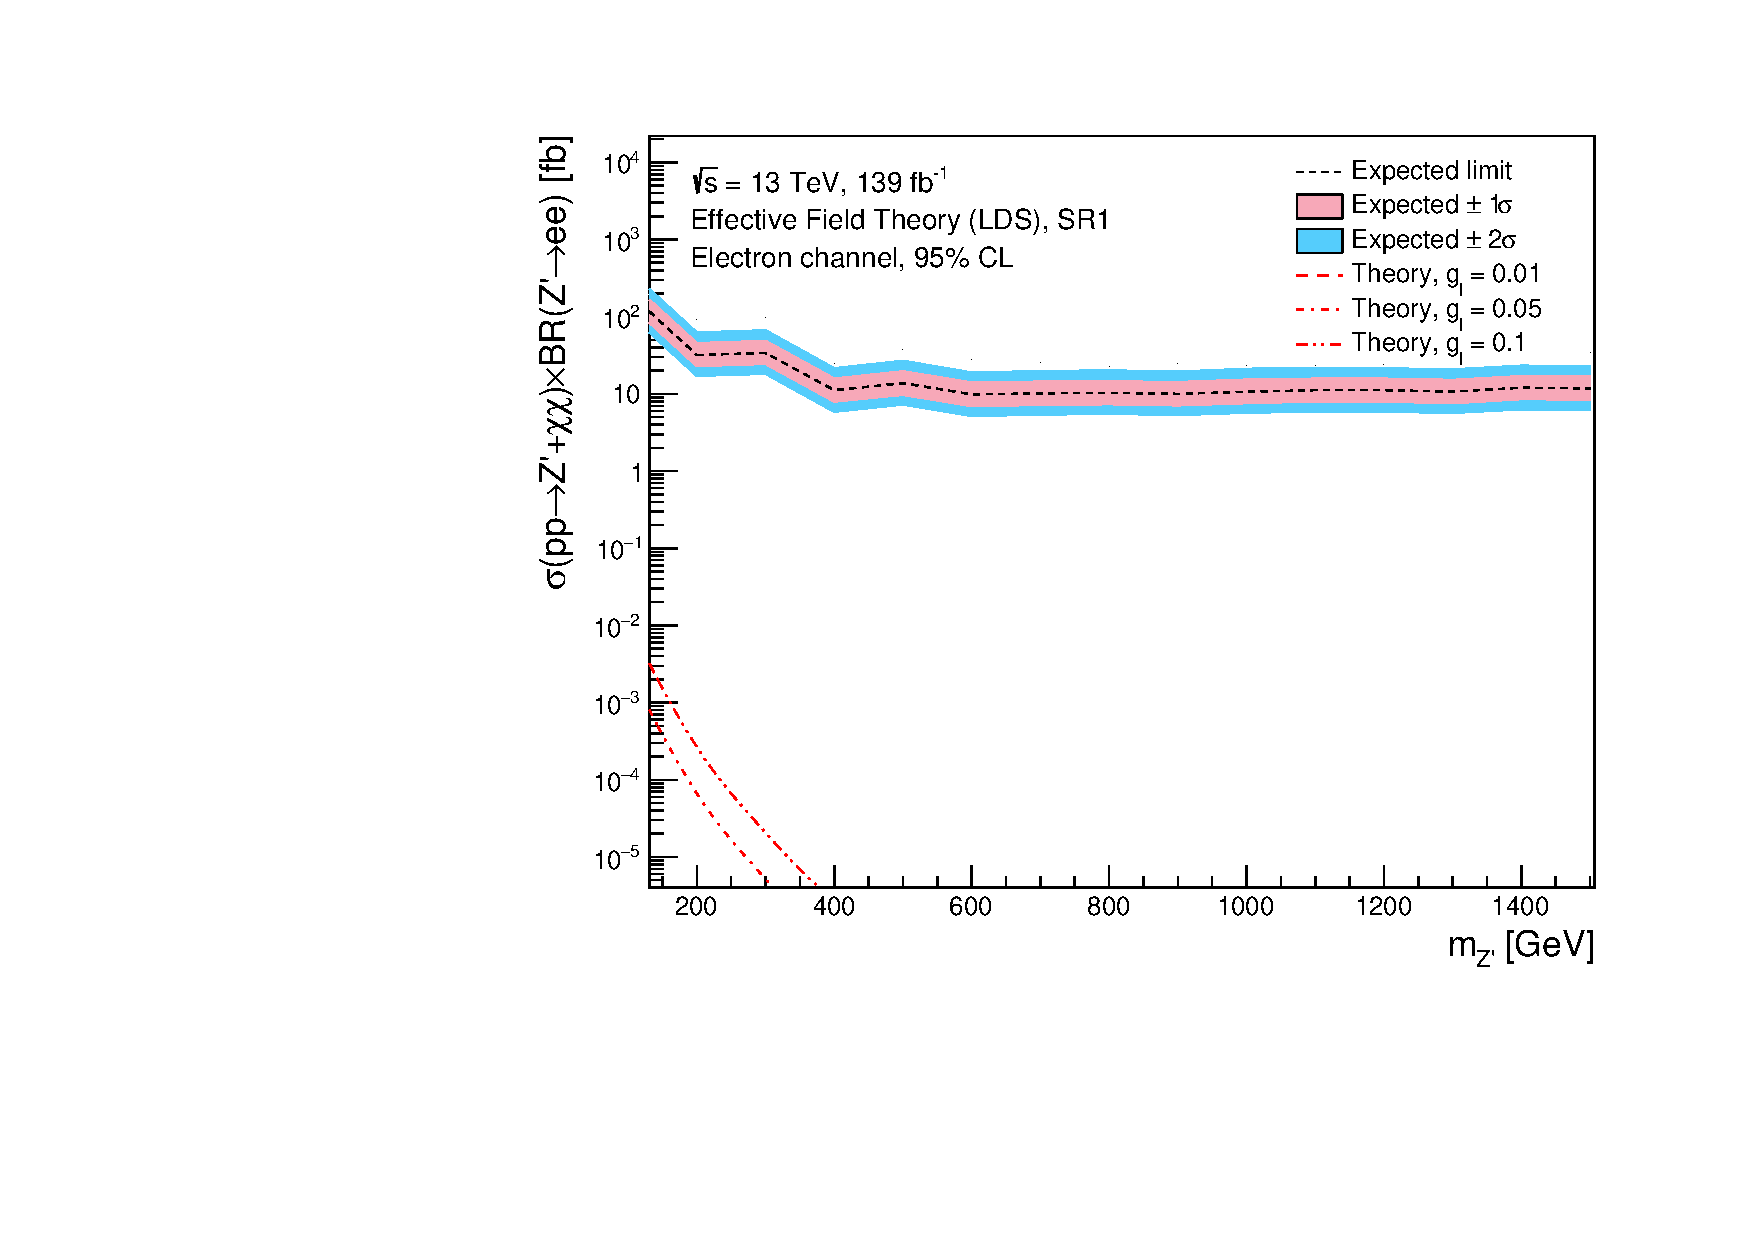
\includegraphics[width=1\textwidth]{Limits/Model_independent/50-100/EFT_LDS/mass_exclusion_ee.pdf}
   \end{subfigure}
   \hfill
   \begin{subfigure}[b]{0.49\textwidth}
      \centering
      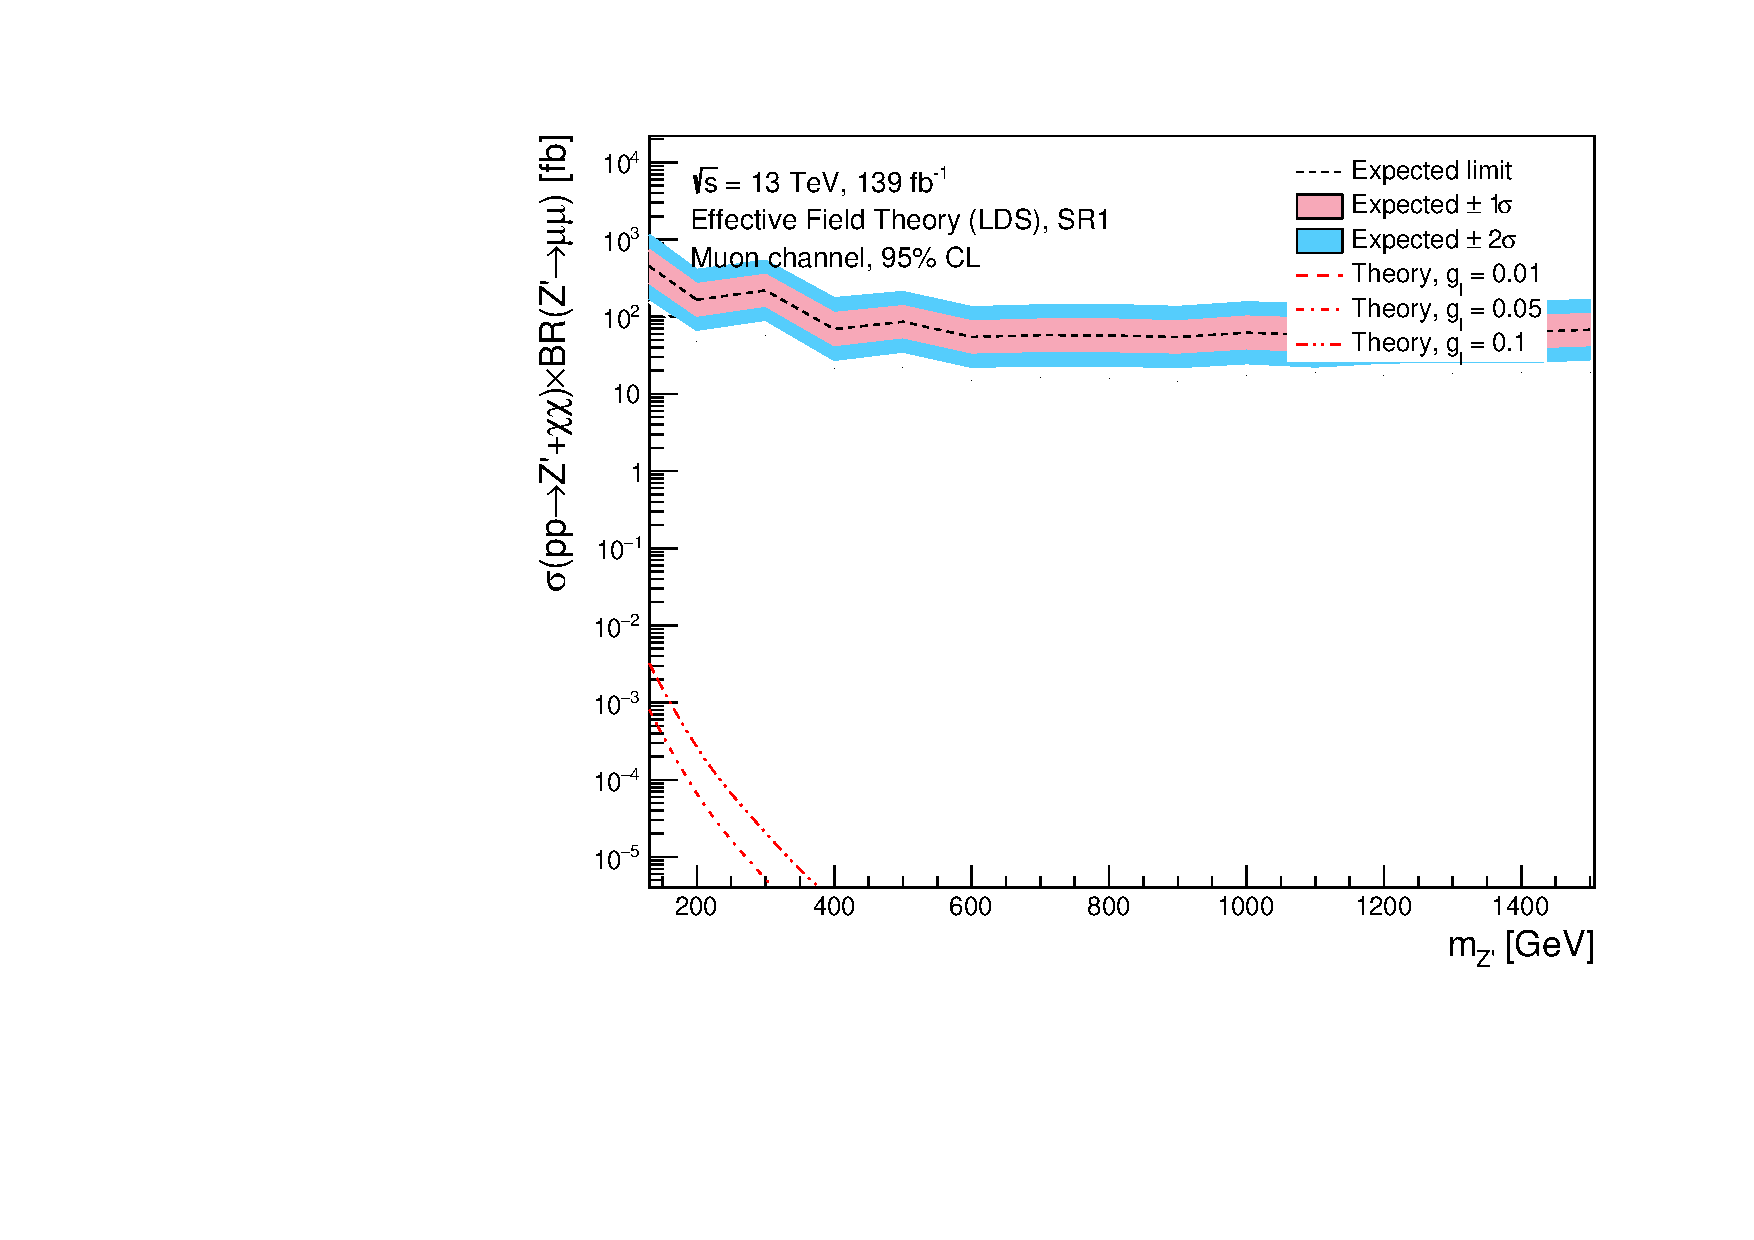
\includegraphics[width=1\textwidth]{Limits/Model_independent/50-100/EFT_LDS/mass_exclusion_uu.pdf}
   \end{subfigure}
   \hfill
   \begin{subfigure}[b]{0.49\textwidth}
      \centering
      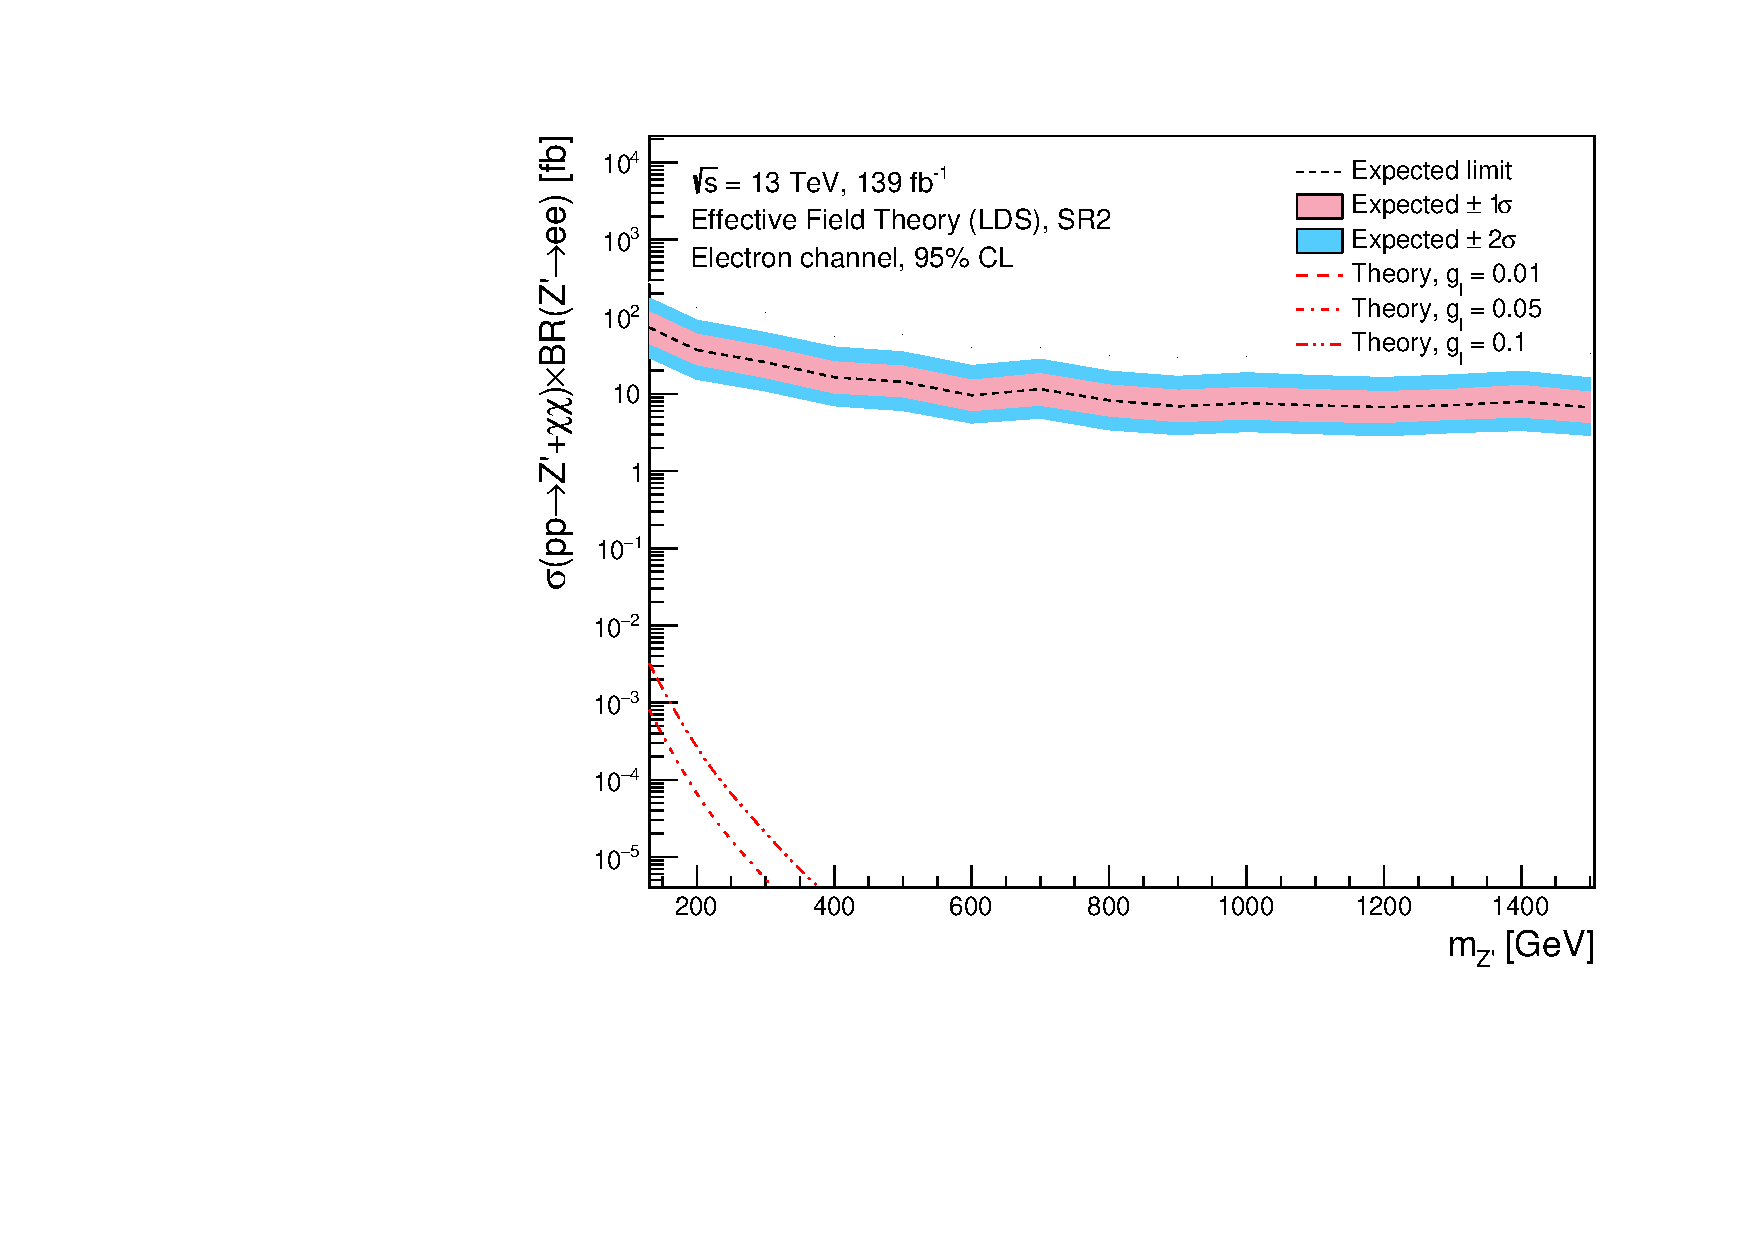
\includegraphics[width=1\textwidth]{Limits/Model_independent/100-150/EFT_LDS/mass_exclusion_ee.pdf}
   \end{subfigure}
   \hfill
   \begin{subfigure}[b]{0.49\textwidth}
      \centering
      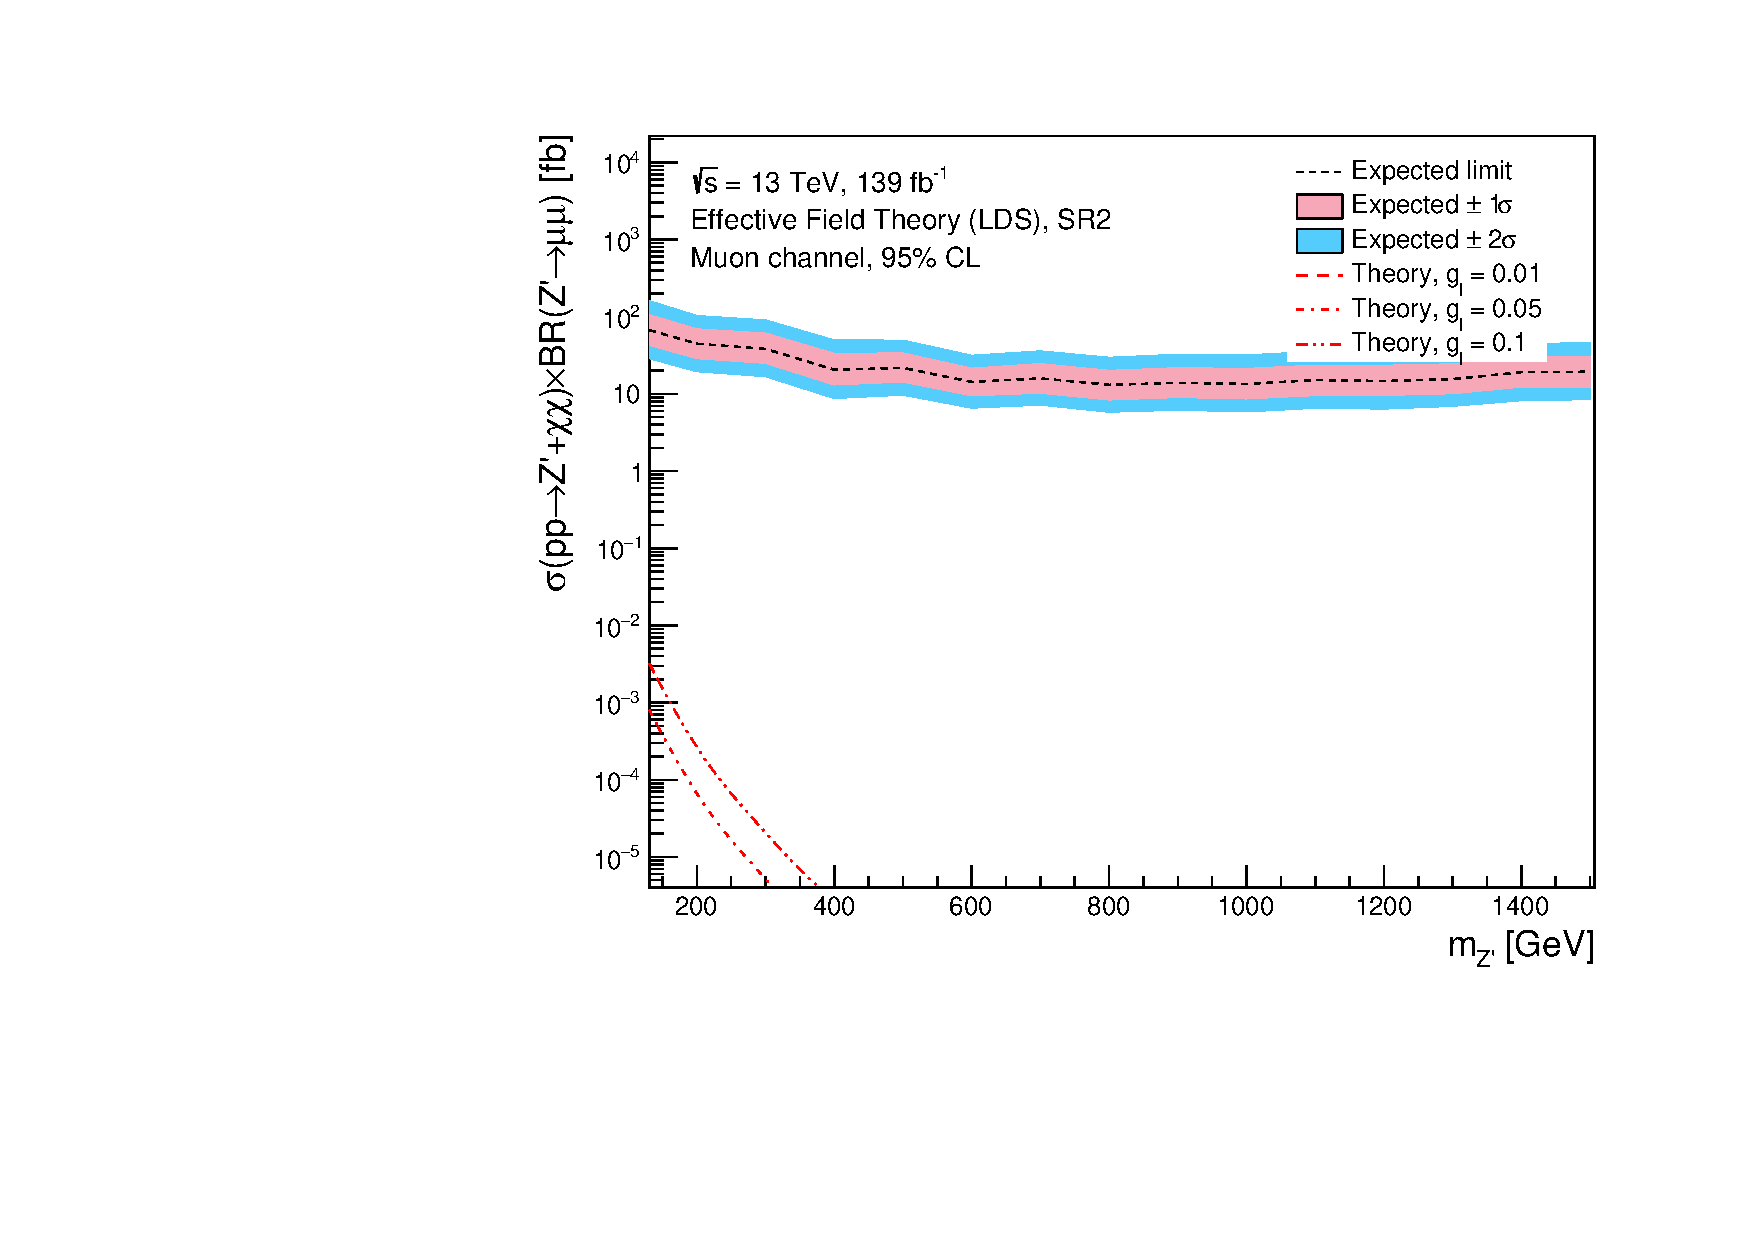
\includegraphics[width=1\textwidth]{Limits/Model_independent/100-150/EFT_LDS/mass_exclusion_uu.pdf}
   \end{subfigure}
   \hfill
	\begin{subfigure}[b]{0.49\textwidth}
      \centering
      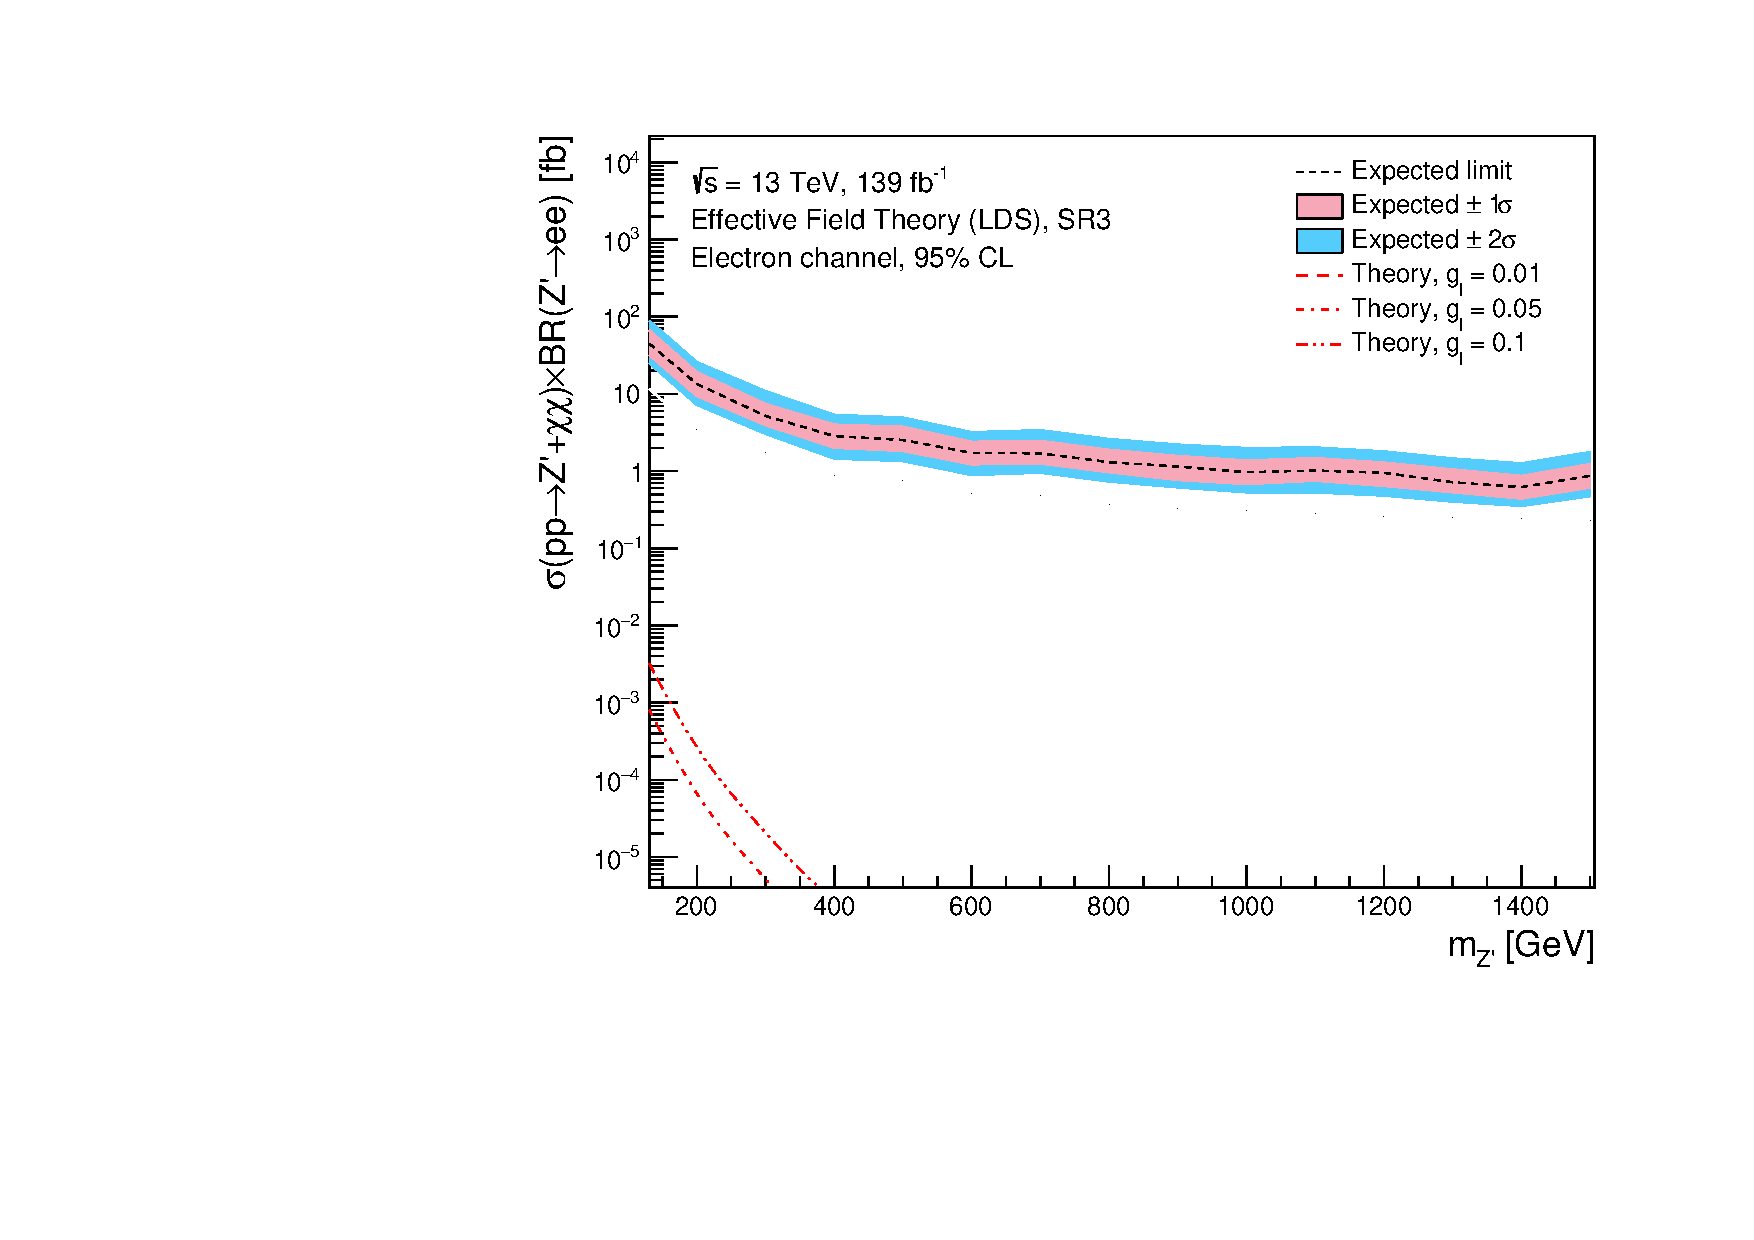
\includegraphics[width=1\textwidth]{Limits/Model_independent/150/EFT_LDS/mass_exclusion_ee.pdf}
   \end{subfigure}
   \hfill
   \begin{subfigure}[b]{0.49\textwidth}
      \centering
      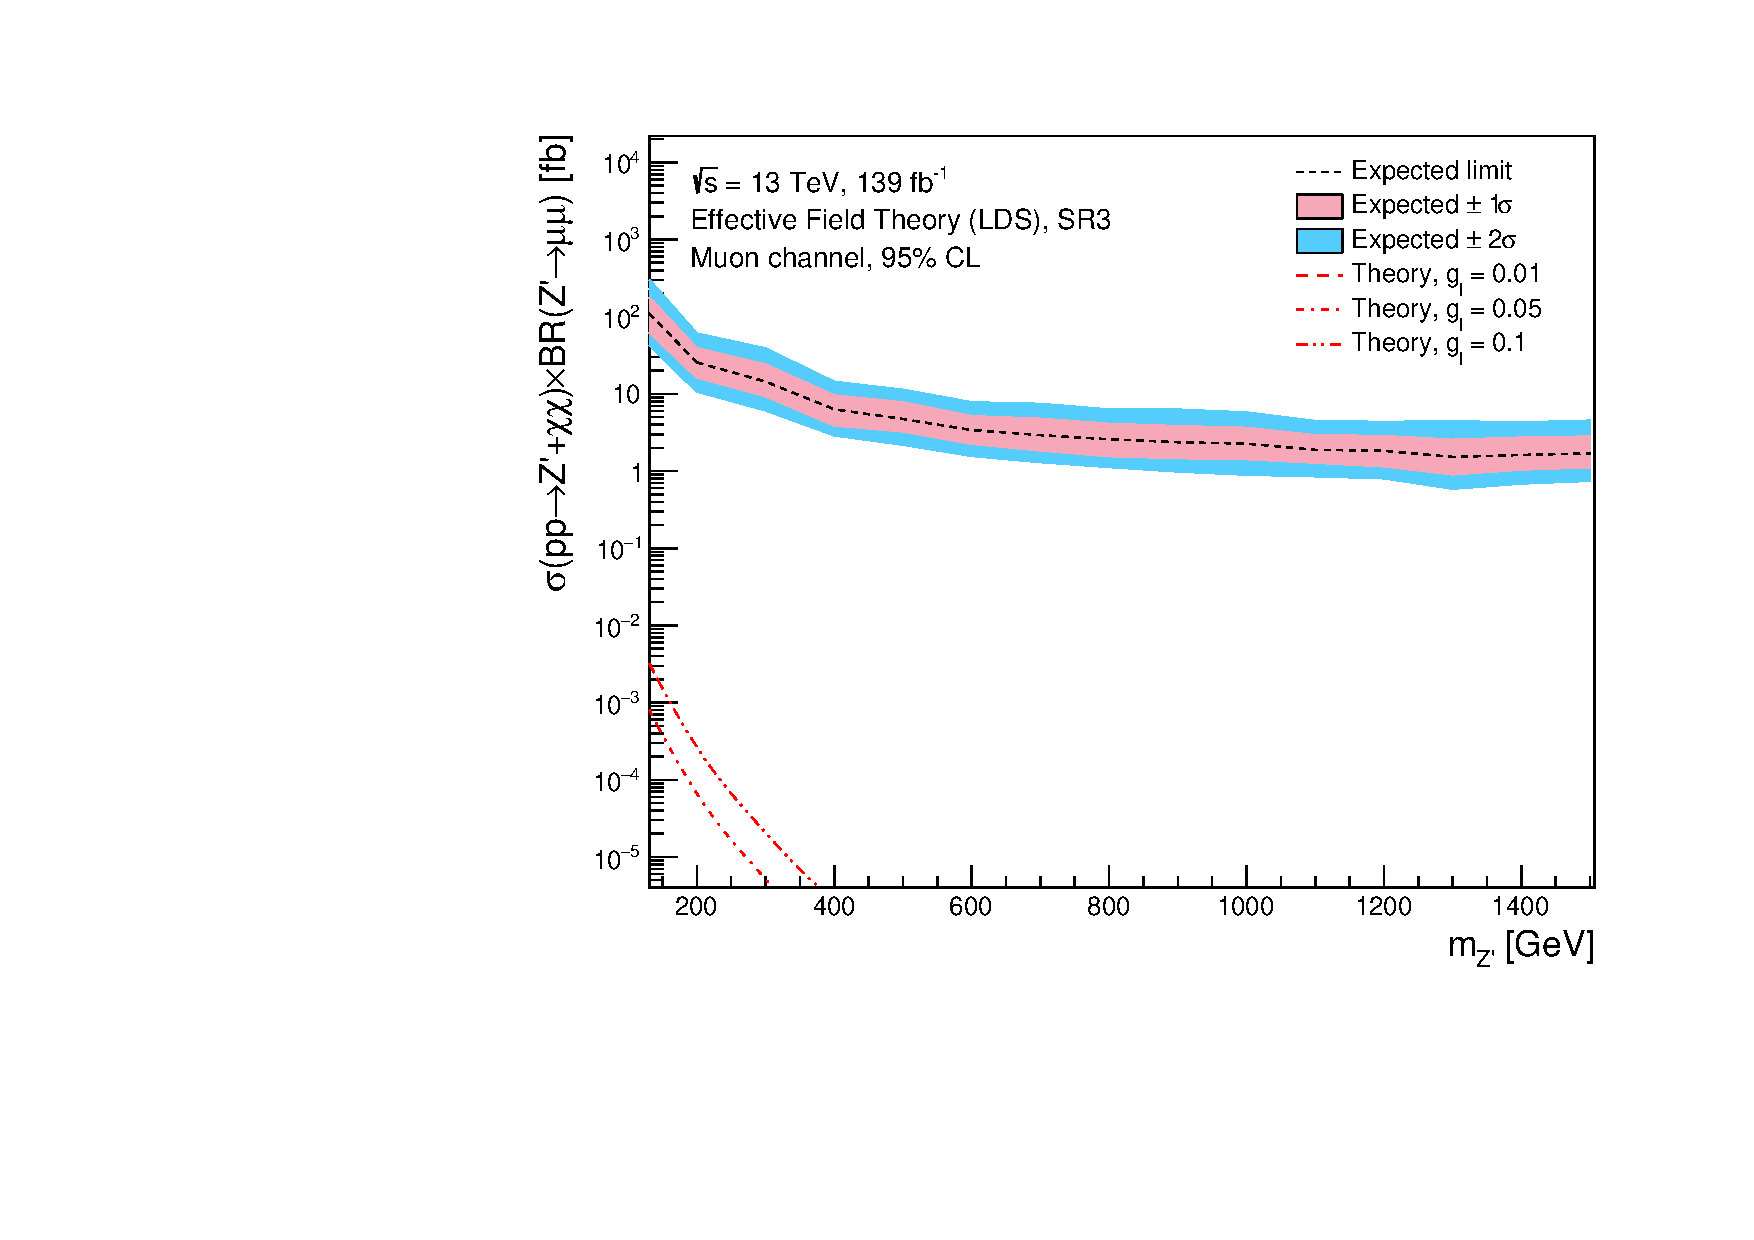
\includegraphics[width=1\textwidth]{Limits/Model_independent/150/EFT_LDS/mass_exclusion_uu.pdf}
   \end{subfigure}
   \caption[Expected mass exclusion limits results for EFT LDS model on $ee$ and $\mu\mu$ channel using the model independent approach]{Mass exclusion limits of $ee$ (left) and $\mu\mu$ (right) channel for Z' EFT Light Dark Sector model using the model independent approach. To remind what the SRs are: SR1 has $E_T^{miss}\in[50, 100]$ GeV, SR2 has $E_T^{miss}\in[100, 150]$ GeV, and SR3 has $E_T^{miss}>150$ GeV. The y-axis of both plots represents the cross-section times branching ratio of the process we are studying. The x-axis is the mass of the $Z'$ boson. We did not interpolate between the available masses we had simulated, 
   and have rather just connected the values calculated for each mass point by connecting the points. The dashed black line is the expected 95\% CL limit with a 1$\sigma$ and 2$\sigma$ variance. 
   The different red dashed lines represent the theoretical cross-section times branching ratio of the process when varying the value of the lepton coupling $g_l$ between the leptons and the $Z'$ boson. The simulated events in this thesis utilized the value $g_l=$ 0.01, we include the cross-section times branching ratio when increasing this coupling to 0.05 and 0.1 to see how the exclusions change.  }\label{fig:EFT_LDS_me_SRS}
\end{figure}


\clearpage
\section{Direct slepton production}
\begin{figure}[!ht]
	\centering
   \begin{subfigure}[b]{0.49\textwidth}
      \centering
      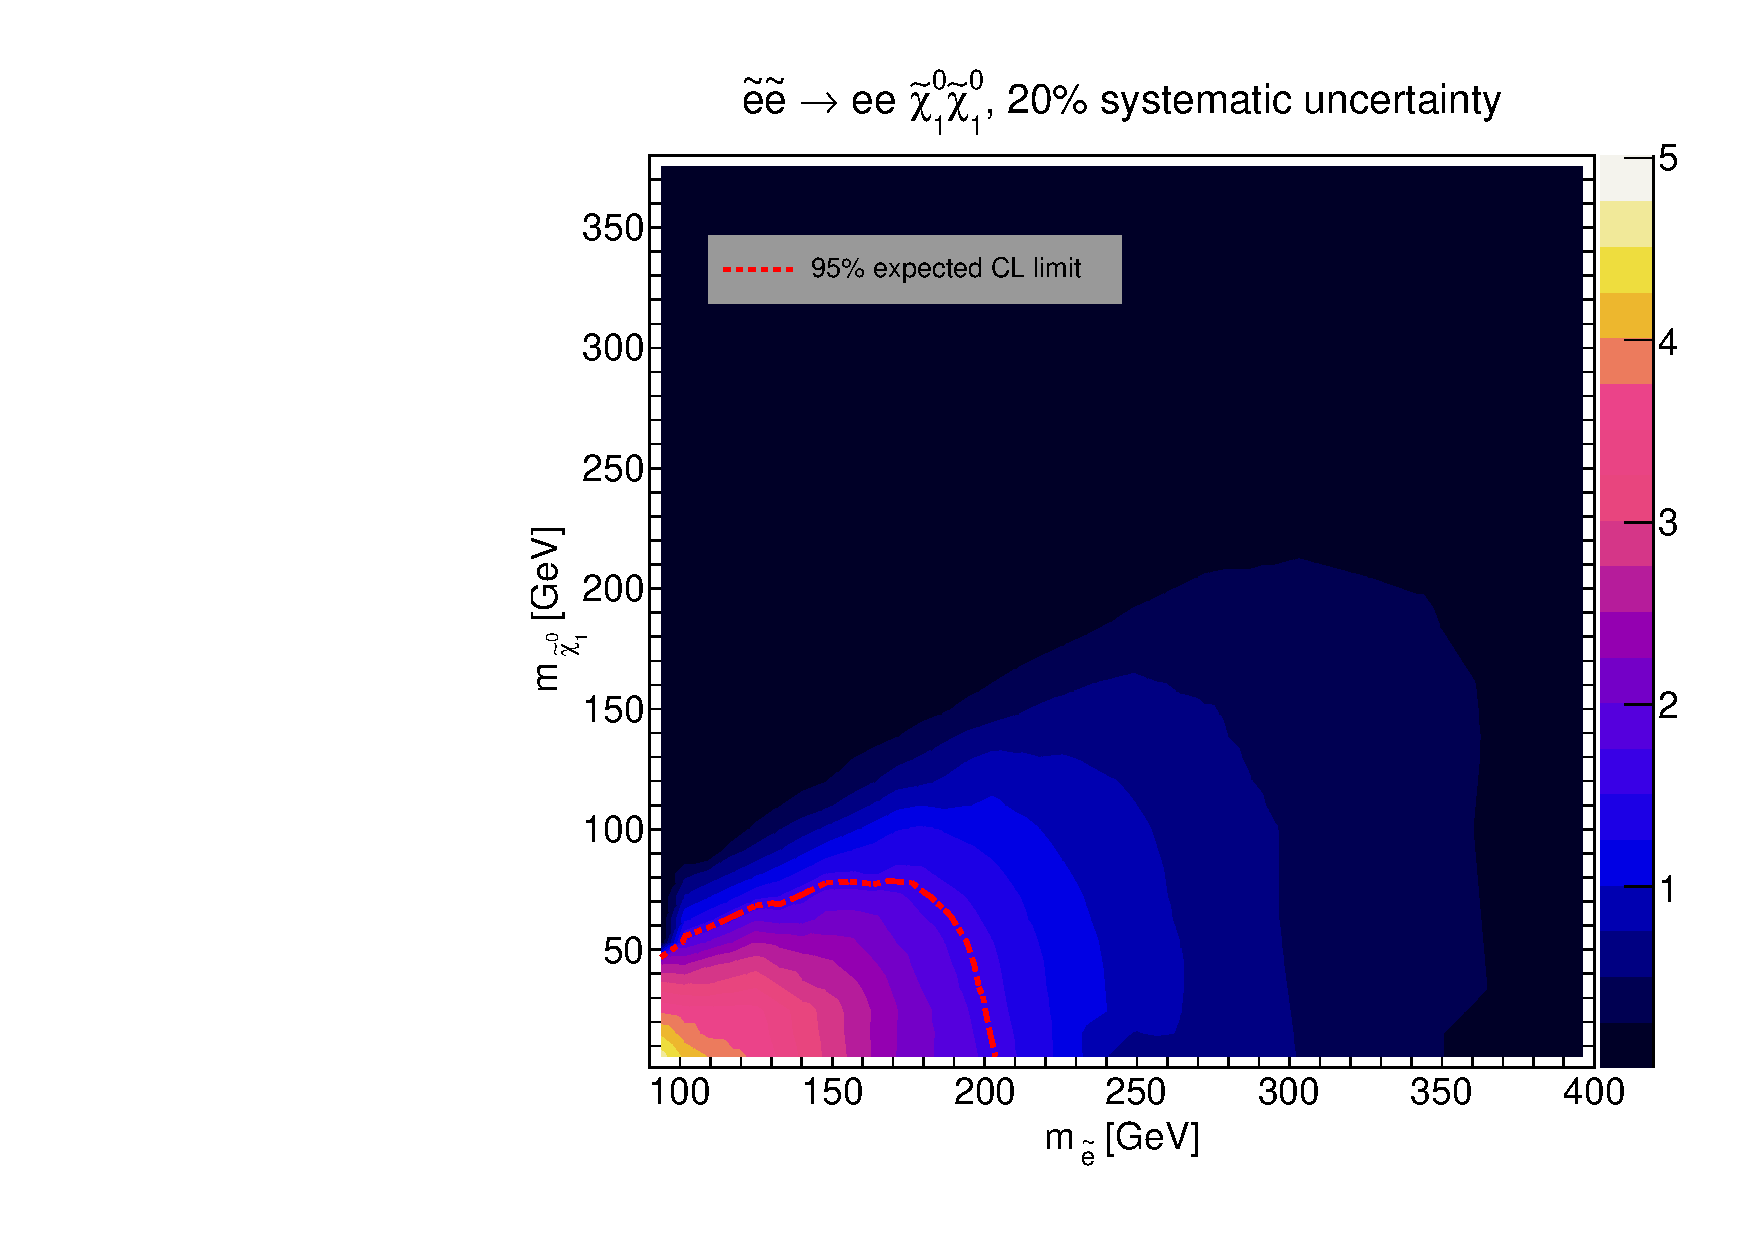
\includegraphics[width=1\textwidth]{Limits/SlepSlep/SlepSlep_ee.pdf}
      \end{subfigure}
   \hfill
   \begin{subfigure}[b]{0.49\textwidth}
      \centering
      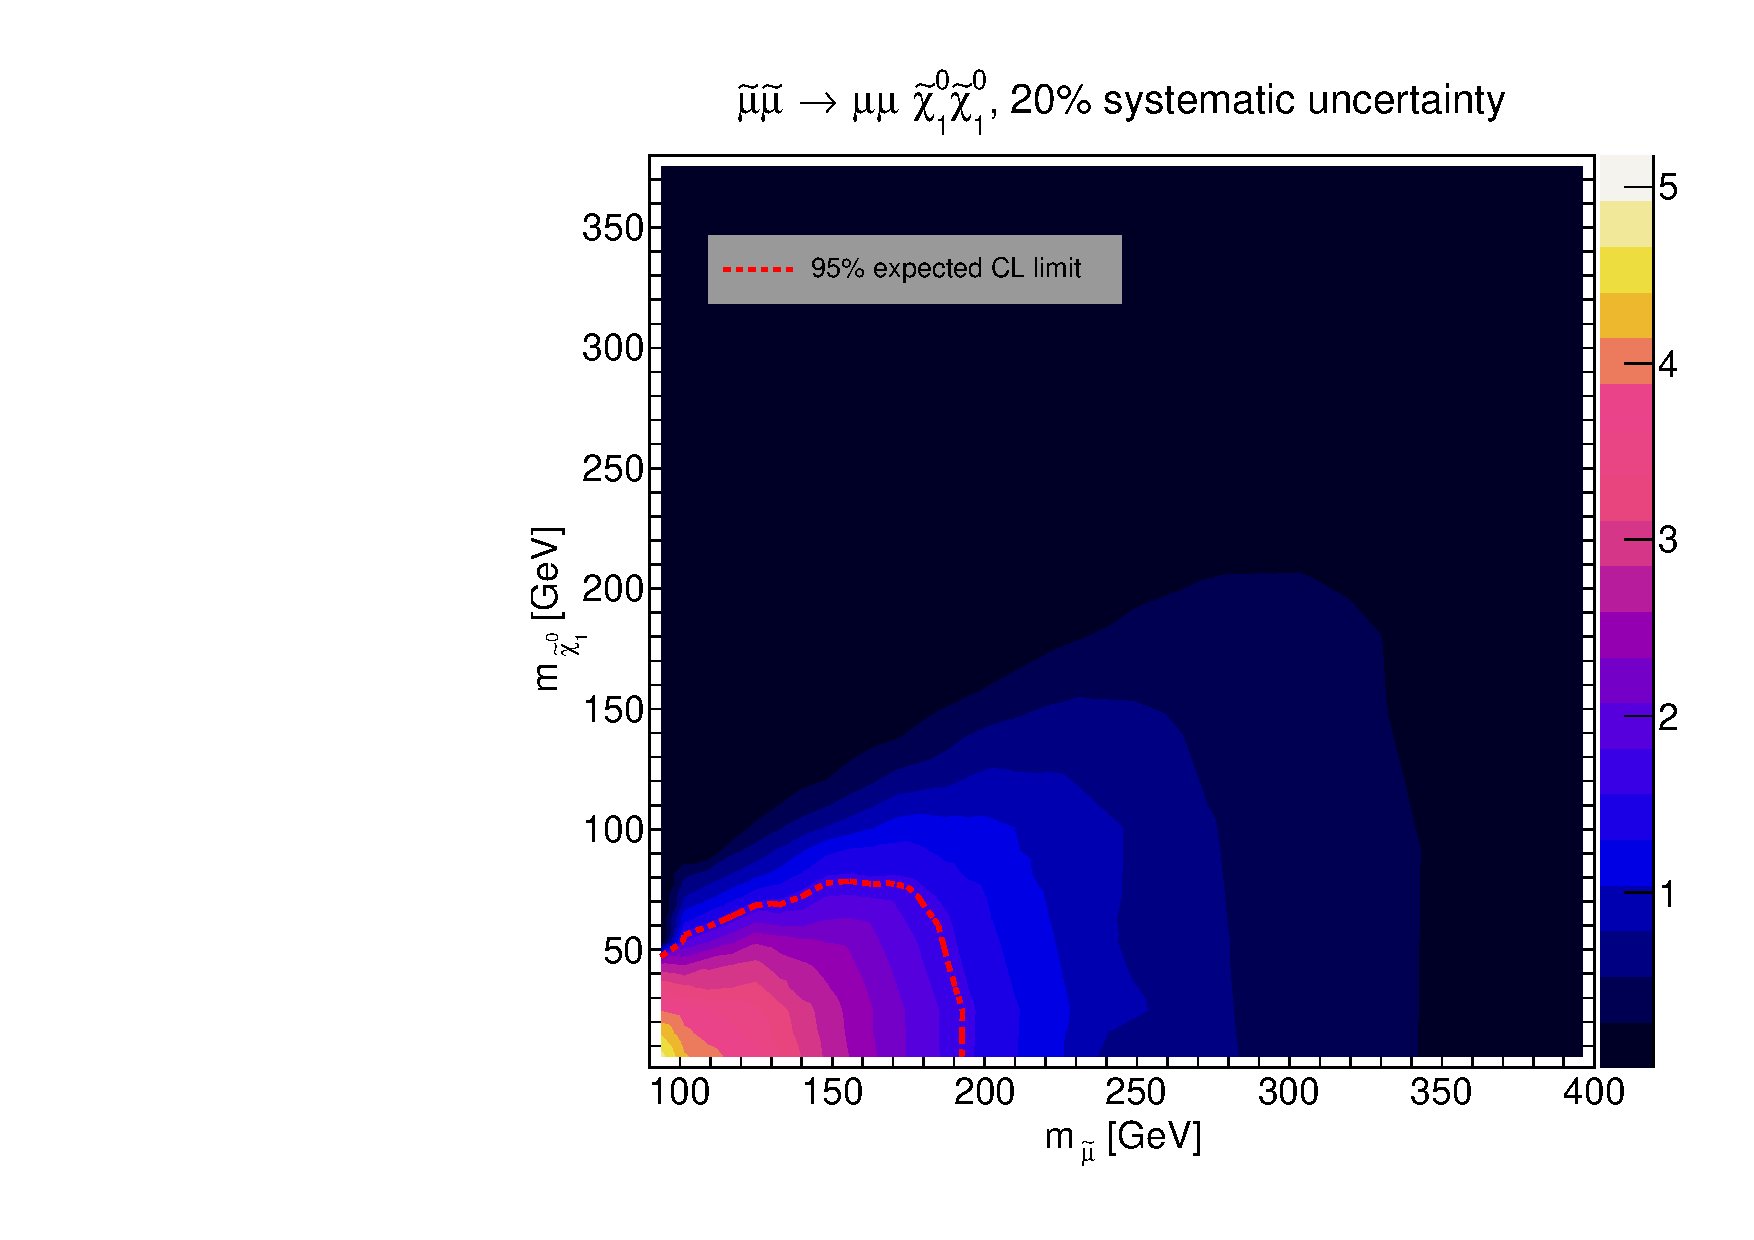
\includegraphics[width=1\textwidth]{Limits/SlepSlep/SlepSlep_uu.pdf}
      \end{subfigure}
   \caption[Expected mass exclusion limits of $ee$ and $\mu\mu$ channel for all direct slepton production model using the model dependent approach]{Mass exclusion limits of $ee$ (left) and $\mu\mu$ (right) channel for direct slepton production model using the model dependent approach. 
   The plots here have the two varying masses as the axes, the z-axis is the expected significance calculated using Eq. (\ref{eq:significance}) with uncertainties. The expected 95\% CL limit was chosen using Frequentist statistics using the significance $Z=$ 1.645.   
   We have the slepton mass, $m_{\tilde{\ell}}$, on the x-axis, and the neutralino mass on $m_{\tilde{\chi}_1^0}$ the y-axis.}
\end{figure}

\begin{figure}[!ht]
	\centering
	\begin{subfigure}[b]{0.49\textwidth}
      \centering
      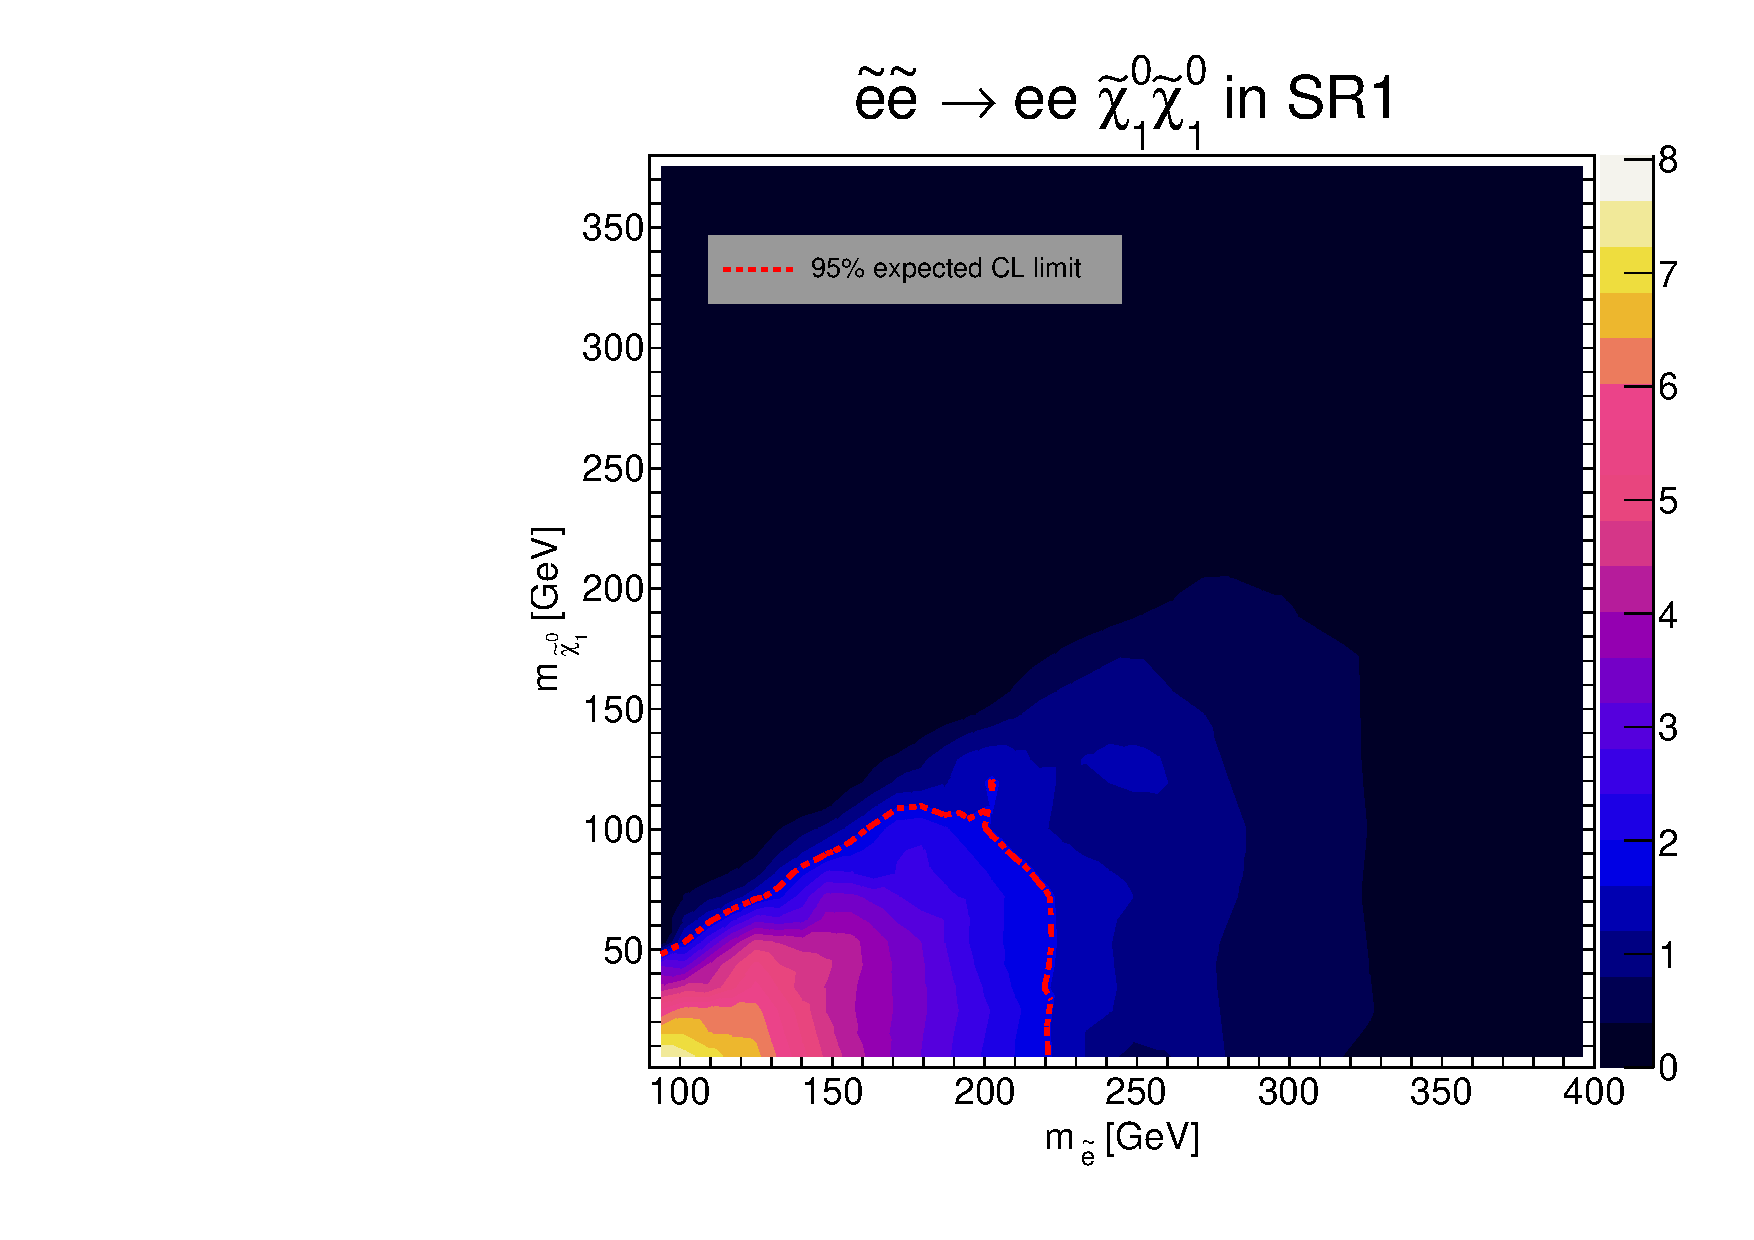
\includegraphics[width=1\textwidth]{Limits/Model_independent/50-100/SlepSlep/SlepSlep_ee.pdf}
   \end{subfigure}
   \hfill
   \begin{subfigure}[b]{0.49\textwidth}
      \centering
      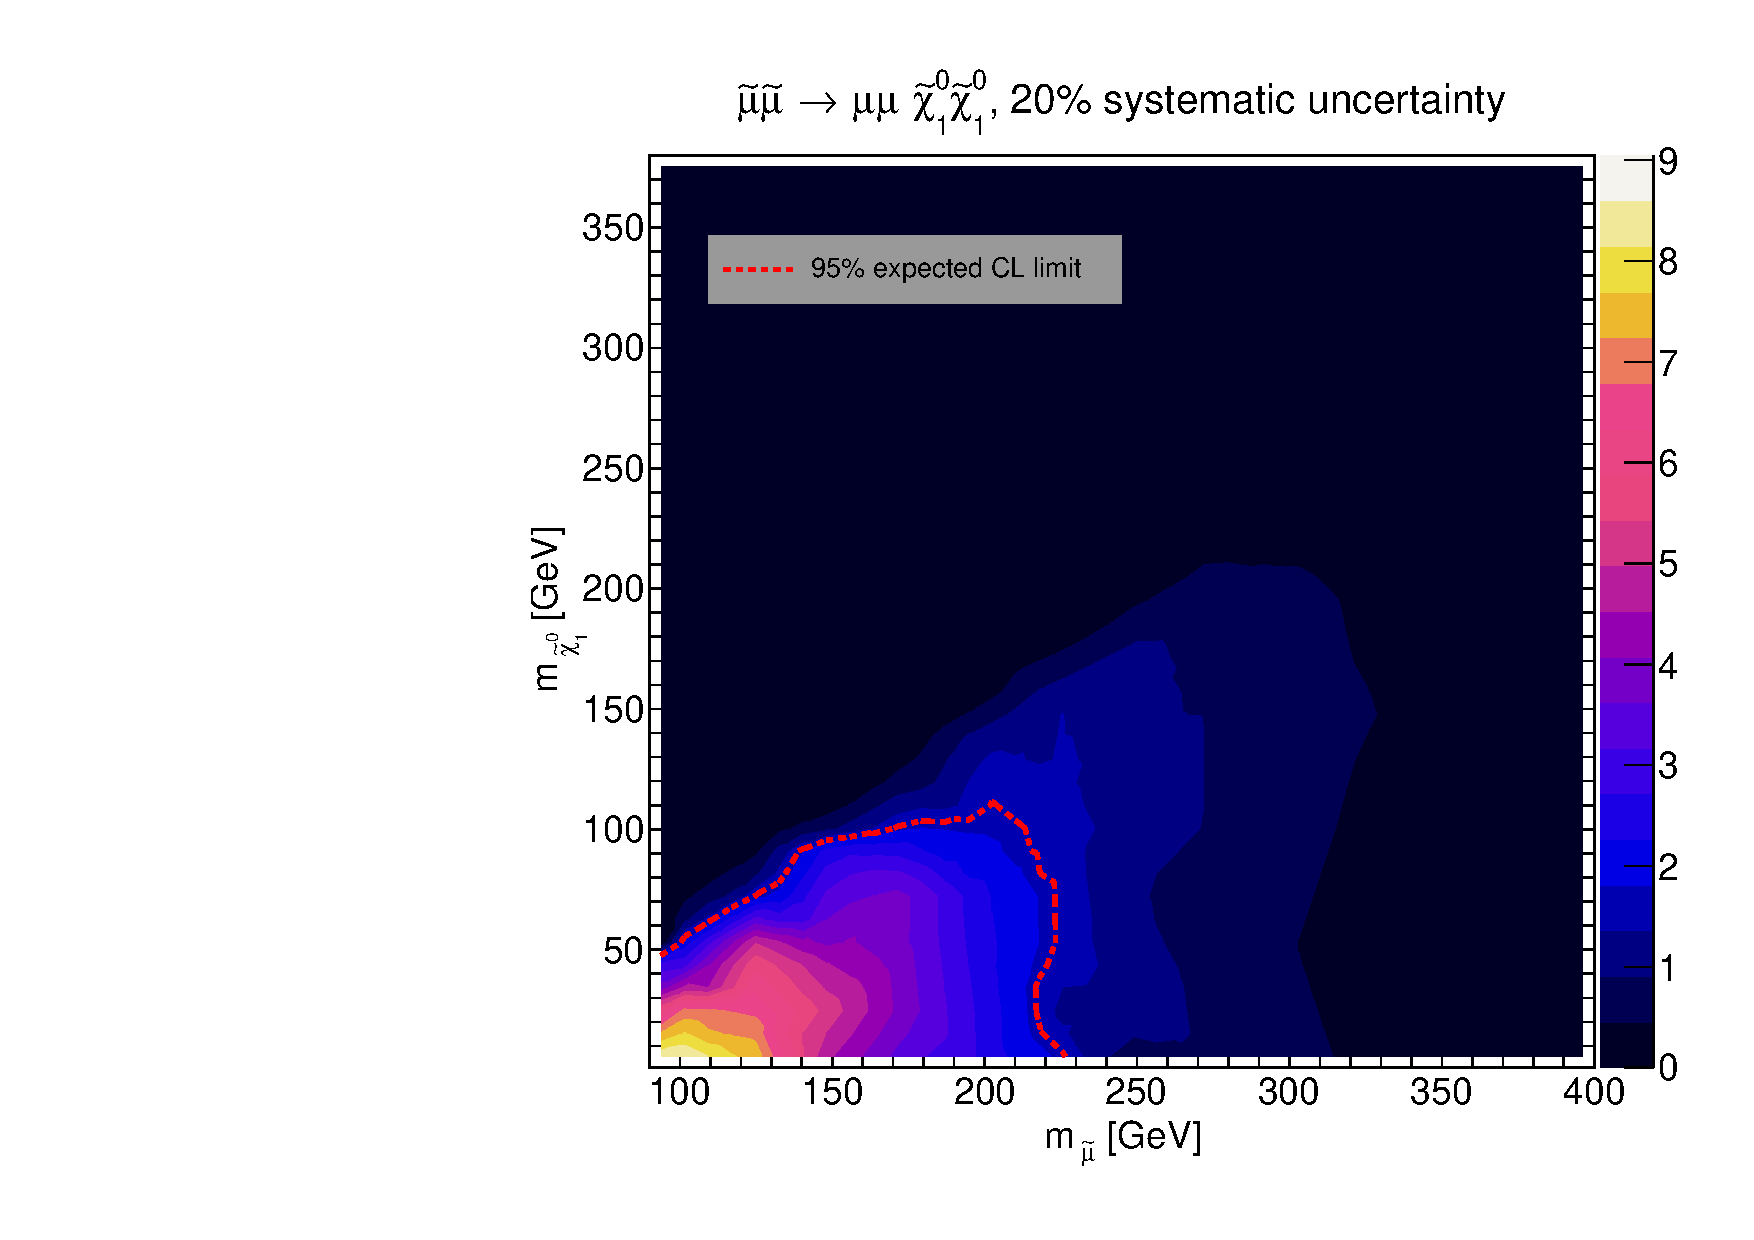
\includegraphics[width=1\textwidth]{Limits/Model_independent/50-100/SlepSlep/SlepSlep_uu.pdf}
   \end{subfigure}
   \hfill
   \begin{subfigure}[b]{0.49\textwidth}
      \centering
      \includegraphics[width=1\textwidth]{Limits/Model_independent/100-150/SlepSlep/SlepSlep_ee.pdf}
   \end{subfigure}
   \hfill
   \begin{subfigure}[b]{0.49\textwidth}
      \centering
      \includegraphics[width=1\textwidth]{Limits/Model_independent/100-150/SlepSlep/SlepSlep_uu.pdf}
   \end{subfigure}
   \hfill
	\begin{subfigure}[b]{0.49\textwidth}
      \centering
      \includegraphics[width=1\textwidth]{Limits/Model_independent/150/SlepSlep/SlepSlep_ee.pdf}
   \end{subfigure}
   \hfill
   \begin{subfigure}[b]{0.49\textwidth}
      \centering
      \includegraphics[width=1\textwidth]{Limits/Model_independent/150/SlepSlep/SlepSlep_uu.pdf}
   \end{subfigure}
   \caption[Expected mass exclusion limits results for direct slepton production model on $ee$ and $\mu\mu$ channel using the model independent approach]{Mass exclusion limits of $ee$ (left) and $\mu\mu$ (right) channel for direct slepton production model using the model independent approach. To remind what the SRs are: SR1 has $E_T^{miss}\in[50, 100]$ GeV, SR2 has $E_T^{miss}\in[100, 150]$ GeV, and SR3 has $E_T^{miss}>150$ GeV. 
   The plots here have the two varying masses as the axes, the z-axis is the expected significance calculated using Eq. (\ref{eq:significance}) with uncertainties. The expected 95\% CL limit was chosen using Frequentist statistics using the significance $Z=$ 1.645.   
   We have the slepton mass, $m_{\tilde{\ell}}$, on the x-axis, and the neutralino mass on $m_{\tilde{\chi}_1^0}$ the y-axis.}
\end{figure}


\clearpage
\section{2HDM + a}
\subsection{Setting $\tan\beta=1$}
\begin{figure}[!ht]
	\centering
   \begin{subfigure}[b]{0.49\textwidth}
      \centering
      \includegraphics[width=1\textwidth]{Limits/2HDM/2HDM_ee_tb1.pdf}
      \end{subfigure}
   \hfill
   \begin{subfigure}[b]{0.49\textwidth}
      \centering
      \includegraphics[width=1\textwidth]{Limits/2HDM/2HDM_uu_tb1.pdf}
      \end{subfigure}
   \caption[Expected mass exclusion limits of $ee$ and $\mu\mu$ channel for all 2HDM + a model with $\tan\beta=1$ model using the model dependent approach]{Mass exclusion limits of $ee$ (left) and $\mu\mu$ (right) channel for 2HDM + a model with $\tan\beta=1$ using the model dependent approach. 
   The plots here have the two varying masses as the axes, the z-axis is the expected significance calculated using Eq. (\ref{eq:significance}) with uncertainties. The expected 95\% CL limit was chosen using Frequentist statistics using the significance $Z=$ 1.645.   
   We have the charged Higgs mass, $m_{H^-}$, on the x-axis, and the pseudoscalar $a$ mass $m_{a}$ on the y-axis.}
\end{figure}

\begin{figure}[!ht]
	\centering
	\begin{subfigure}[b]{0.49\textwidth}
      \centering
      \includegraphics[width=1\textwidth]{Limits/Model_independent/50-100/2HDM/2HDM_ee_tb1.pdf}
   \end{subfigure}
   \hfill
   \begin{subfigure}[b]{0.49\textwidth}
      \centering
      \includegraphics[width=1\textwidth]{Limits/Model_independent/50-100/2HDM/2HDM_uu_tb1.pdf}
   \end{subfigure}
   \hfill
   \begin{subfigure}[b]{0.49\textwidth}
      \centering
      \includegraphics[width=1\textwidth]{Limits/Model_independent/100-150/2HDM/2HDM_ee_tb1.pdf}
   \end{subfigure}
   \hfill
   \begin{subfigure}[b]{0.49\textwidth}
      \centering
      \includegraphics[width=1\textwidth]{Limits/Model_independent/100-150/2HDM/2HDM_uu_tb1.pdf}
   \end{subfigure}
   \hfill
	\begin{subfigure}[b]{0.49\textwidth}
      \centering
      \includegraphics[width=1\textwidth]{Limits/Model_independent/150/2HDM/2HDM_ee_tb1.pdf}
   \end{subfigure}
   \hfill
   \begin{subfigure}[b]{0.49\textwidth}
      \centering
      \includegraphics[width=1\textwidth]{Limits/Model_independent/150/2HDM/2HDM_uu_tb1.pdf}
   \end{subfigure}
   \caption[Expected mass exclusion limits results for the 2HDM + a model with $\tan\beta=5$ on $ee$ and $\mu\mu$ channel using the model independent approach]{Mass exclusion limits of $ee$ (left) and $\mu\mu$ (right) channel for 2HDM + a model with $\tan\beta=1$ using the model independent approach. To remind what the SRs are: SR1 has $E_T^{miss}\in[50, 100]$ GeV, SR2 has $E_T^{miss}\in[100, 150]$ GeV, and SR3 has $E_T^{miss}>150$ GeV. The plots here have the two varying masses as the axes, the z-axis is the expected significance calculated using Eq. (\ref{eq:significance}) with uncertainties. The expected 95\% CL limit was chosen using Frequentist statistics using the significance $Z=$ 1.645.   
   We have the charged Higgs mass, $m_{H^-}$, on the x-axis, and the pseudoscalar $a$ mass $m_{a}$ on the y-axis.}
\end{figure}

\clearpage
\subsection{Setting $\tan\beta=5$}
\begin{figure}[!ht]
	\centering
   \begin{subfigure}[b]{0.49\textwidth}
      \centering
      \includegraphics[width=1\textwidth]{Limits/2HDM/2HDM_ee_tb5.pdf}
      \end{subfigure}
   \hfill
   \begin{subfigure}[b]{0.49\textwidth}
      \centering
      \includegraphics[width=1\textwidth]{Limits/2HDM/2HDM_uu_tb5.pdf}
      \end{subfigure}
   \caption[Expected mass exclusion limits of $ee$ and $\mu\mu$ channel for 2HDM + a model with $\tan\beta=5$ using the model dependent approach]{Mass exclusion limits of $ee$ (left) and $\mu\mu$ (right) channel for 2HDM + a model with $\tan\beta=5$ using the model dependent approach. The y-axis of both plots represents the cross-section times branching ratio of the process we are studying. The x-axis is the mass of the $Z'$ boson. We did not interpolate between the available masses we had simulated, 
   and have rather just connected the values calculated for each mass point by connecting the points. The dashed black line is the expected 95\% CL limit with a 1$\sigma$ and 2$\sigma$ variance. 
   The different red dashed lines represent the theoretical cross-section times branching ratio of the process when varying the value of the lepton coupling $g_l$ between the leptons and the $Z'$ boson. The simulated events in this thesis utilized the value $g_l=$ 0.01, we include the cross-section times branching ratio when increasing this coupling to 0.05 and 0.1 to see how the exclusions change.  }
\end{figure}

\begin{figure}[!ht]
	\centering
	\begin{subfigure}[b]{0.49\textwidth}
      \centering
      \includegraphics[width=1\textwidth]{Limits/Model_independent/50-100/2HDM/2HDM_ee_tb5.pdf}
   \end{subfigure}
   \hfill
   \begin{subfigure}[b]{0.49\textwidth}
      \centering
      \includegraphics[width=1\textwidth]{Limits/Model_independent/50-100/2HDM/2HDM_uu_tb5.pdf}
   \end{subfigure}
   \hfill
   \begin{subfigure}[b]{0.49\textwidth}
      \centering
      \includegraphics[width=1\textwidth]{Limits/Model_independent/100-150/2HDM/2HDM_ee_tb5.pdf}
   \end{subfigure}
   \hfill
   \begin{subfigure}[b]{0.49\textwidth}
      \centering
      \includegraphics[width=1\textwidth]{Limits/Model_independent/100-150/2HDM/2HDM_uu_tb5.pdf}
   \end{subfigure}
   \hfill
	\begin{subfigure}[b]{0.49\textwidth}
      \centering
      \includegraphics[width=1\textwidth]{Limits/Model_independent/150/2HDM/2HDM_ee_tb5.pdf}
   \end{subfigure}
   \hfill
   \begin{subfigure}[b]{0.49\textwidth}
      \centering
      \includegraphics[width=1\textwidth]{Limits/Model_independent/150/2HDM/2HDM_uu_tb5.pdf}
   \end{subfigure}
   \caption[Expected mass exclusion limits results for 2HDM + a model with $\tan\beta=5$ on $ee$ and $\mu\mu$ channel using the model independent approach]{Mass exclusion limits of $ee$ (left) and $\mu\mu$ (right) channel for 2HDM + a model with $\tan\beta=5$ using the model independent approach. To remind what the SRs are: SR1 has $E_T^{miss}\in[50, 100]$ GeV, SR2 has $E_T^{miss}\in[100, 150]$ GeV, and SR3 has $E_T^{miss}>150$ GeV. The plots here have the two varying masses as the axes, the z-axis is the expected significance calculated using Eq. (\ref{eq:significance}) with uncertainties. The expected 95\% CL limit was chosen using Frequentist statistics using the significance $Z=$ 1.645.   
   We have the charged Higgs mass, $m_{H^-}$, on the x-axis, and the pseudoscalar $a$ mass $m_{a}$ on the y-axis.}
\end{figure}

\clearpage
\subsection{Setting $\tan\beta=10$}
\begin{figure}[!ht]
	\centering
   \begin{subfigure}[b]{0.49\textwidth}
      \centering
      \includegraphics[width=1\textwidth]{Limits/2HDM/2HDM_ee_tb10.pdf}
      \end{subfigure}
   \hfill
   \begin{subfigure}[b]{0.49\textwidth}
      \centering
      \includegraphics[width=1\textwidth]{Limits/2HDM/2HDM_uu_tb10.pdf}
      \end{subfigure}
   \caption[Expected mass exclusion limits of $ee$ and $\mu\mu$ channel for all 2HDM + a model with $\tan\beta=10$ using the model dependent approach]{Mass exclusion limits of $ee$ (left) and $\mu\mu$ (right) channel for 2HDM + a model with $\tan\beta=10$ using the model dependent approach. The y-axis of both plots represents the cross-section times branching ratio of the process we are studying. The x-axis is the mass of the $Z'$ boson. We did not interpolate between the available masses we had simulated, 
   and have rather just connected the values calculated for each mass point by connecting the points. The dashed black line is the expected 95\% CL limit with a 1$\sigma$ and 2$\sigma$ variance. 
   The different red dashed lines represent the theoretical cross-section times branching ratio of the process when varying the value of the lepton coupling $g_l$ between the leptons and the $Z'$ boson. The simulated events in this thesis utilized the value $g_l=$ 0.01, we include the cross-section times branching ratio when increasing this coupling to 0.05 and 0.1 to see how the exclusions change.  }
\end{figure}

\begin{figure}[!ht]
	\centering
	\begin{subfigure}[b]{0.49\textwidth}
      \centering
      \includegraphics[width=1\textwidth]{Limits/Model_independent/50-100/2HDM/2HDM_ee_tb10.pdf}
   \end{subfigure}
   \hfill
   \begin{subfigure}[b]{0.49\textwidth}
      \centering
      \includegraphics[width=1\textwidth]{Limits/Model_independent/50-100/2HDM/2HDM_uu_tb10.pdf}
   \end{subfigure}
   \hfill
   \begin{subfigure}[b]{0.49\textwidth}
      \centering
      \includegraphics[width=1\textwidth]{Limits/Model_independent/100-150/2HDM/2HDM_ee_tb10.pdf}
   \end{subfigure}
   \hfill
   \begin{subfigure}[b]{0.49\textwidth}
      \centering
      \includegraphics[width=1\textwidth]{Limits/Model_independent/100-150/2HDM/2HDM_uu_tb10.pdf}
   \end{subfigure}
   \hfill
	\begin{subfigure}[b]{0.49\textwidth}
      \centering
      \includegraphics[width=1\textwidth]{Limits/Model_independent/150/2HDM/2HDM_ee_tb10.pdf}
   \end{subfigure}
   \hfill
   \begin{subfigure}[b]{0.49\textwidth}
      \centering
      \includegraphics[width=1\textwidth]{Limits/Model_independent/150/2HDM/2HDM_uu_tb10.pdf}
   \end{subfigure}
   \caption[Expected mass exclusion limits results for 2HDM + a model with $\tan\beta=10$ on $ee$ and $\mu\mu$ channel using the model independent approach]{Mass exclusion limits of $ee$ (left) and $\mu\mu$ (right) channel for 2HDM + a model with $\tan\beta=10$ using the model independent approach. To remind what the SRs are: SR1 has $E_T^{miss}\in[50, 100]$ GeV, SR2 has $E_T^{miss}\in[100, 150]$ GeV, and SR3 has $E_T^{miss}>150$ GeV. The plots here have the two varying masses as the axes, the z-axis is the expected significance calculated using Eq. (\ref{eq:significance}) with uncertainties. The expected 95\% CL limit was chosen using Frequentist statistics using the significance $Z=$ 1.645.   
   We have the charged Higgs mass, $m_{H^-}$, on the x-axis, and the pseudoscalar $a$ mass $m_{a}$ on the y-axis.}
\end{figure}

\clearpage
\subsection{Setting $\tan\beta=20$}
\begin{figure}[!ht]
	\centering
   \begin{subfigure}[b]{0.49\textwidth}
      \centering
      \includegraphics[width=1\textwidth]{Limits/2HDM/2HDM_ee_tb20.pdf}
      \end{subfigure}
   \hfill
   \begin{subfigure}[b]{0.49\textwidth}
      \centering
      \includegraphics[width=1\textwidth]{Limits/2HDM/2HDM_uu_tb20.pdf}
      \end{subfigure}
   \caption[Expected mass exclusion limits of $ee$ and $\mu\mu$ channel for all 2HDM + a model with $\tan\beta=20$ using the model dependent approach]{Mass exclusion limits of $ee$ (left) and $\mu\mu$ (right) channel for 2HDM + a model with $\tan\beta=20$ using the model dependent approach. The y-axis of both plots represents the cross-section times branching ratio of the process we are studying. The x-axis is the mass of the $Z'$ boson. We did not interpolate between the available masses we had simulated, 
   and have rather just connected the values calculated for each mass point by connecting the points. The dashed black line is the expected 95\% CL limit with a 1$\sigma$ and 2$\sigma$ variance. 
   The different red dashed lines represent the theoretical cross-section times branching ratio of the process when varying the value of the lepton coupling $g_l$ between the leptons and the $Z'$ boson. The simulated events in this thesis utilized the value $g_l=$ 0.01, we include the cross-section times branching ratio when increasing this coupling to 0.05 and 0.1 to see how the exclusions change.  }
\end{figure}

\begin{figure}[!ht]
	\centering
	\begin{subfigure}[b]{0.49\textwidth}
      \centering
      \includegraphics[width=1\textwidth]{Limits/Model_independent/50-100/2HDM/2HDM_ee_tb20.pdf}
   \end{subfigure}
   \hfill
   \begin{subfigure}[b]{0.49\textwidth}
      \centering
      \includegraphics[width=1\textwidth]{Limits/Model_independent/50-100/2HDM/2HDM_uu_tb20.pdf}
   \end{subfigure}
   \hfill
   \begin{subfigure}[b]{0.49\textwidth}
      \centering
      \includegraphics[width=1\textwidth]{Limits/Model_independent/100-150/2HDM/2HDM_ee_tb20.pdf}
   \end{subfigure}
   \hfill
   \begin{subfigure}[b]{0.49\textwidth}
      \centering
      \includegraphics[width=1\textwidth]{Limits/Model_independent/100-150/2HDM/2HDM_uu_tb20.pdf}
   \end{subfigure}
   \hfill
	\begin{subfigure}[b]{0.49\textwidth}
      \centering
      \includegraphics[width=1\textwidth]{Limits/Model_independent/150/2HDM/2HDM_ee_tb20.pdf}
   \end{subfigure}
   \hfill
   \begin{subfigure}[b]{0.49\textwidth}
      \centering
      \includegraphics[width=1\textwidth]{Limits/Model_independent/150/2HDM/2HDM_uu_tb20.pdf}
   \end{subfigure}
   \caption[Expected mass exclusion limits results for 2HDM + a model with $\tan\beta=20$ on $ee$ and $\mu\mu$ channel using the model independent approach]{Mass exclusion limits of $ee$ (left) and $\mu\mu$ (right) channel for 2HDM + a model with $\tan\beta=20$ using the model independent approach. To remind what the SRs are: SR1 has $E_T^{miss}\in[50, 100]$ GeV, SR2 has $E_T^{miss}\in[100, 150]$ GeV, and SR3 has $E_T^{miss}>150$ GeV. The plots here have the two varying masses as the axes, the z-axis is the expected significance calculated using Eq. (\ref{eq:significance}) with uncertainties. The expected 95\% CL limit was chosen using Frequentist statistics using the significance $Z=$ 1.645.   
   We have the charged Higgs mass, $m_{H^-}$, on the x-axis, and the pseudoscalar $a$ mass $m_{a}$ on the y-axis.}
\end{figure}

\clearpage
\subsection{Setting $\tan\beta=30$}
\begin{figure}[!ht]
	\centering
   \begin{subfigure}[b]{0.49\textwidth}
      \centering
      \includegraphics[width=1\textwidth]{Limits/2HDM/2HDM_ee_tb30.pdf}
      \end{subfigure}
   \hfill
   \begin{subfigure}[b]{0.49\textwidth}
      \centering
      \includegraphics[width=1\textwidth]{Limits/2HDM/2HDM_uu_tb30.pdf}
      \end{subfigure}
   \caption[Expected mass exclusion limits of $ee$ and $\mu\mu$ channel for all 2HDM + a model with $\tan\beta=30$ using the model dependent approach]{Mass exclusion limits of $ee$ (left) and $\mu\mu$ (right) channel for 2HDM + a model with $\tan\beta=30$ using the model dependent approach. The y-axis of both plots represents the cross-section times branching ratio of the process we are studying. The x-axis is the mass of the $Z'$ boson. We did not interpolate between the available masses we had simulated, 
   and have rather just connected the values calculated for each mass point by connecting the points. The dashed black line is the expected 95\% CL limit with a 1$\sigma$ and 2$\sigma$ variance. 
   The different red dashed lines represent the theoretical cross-section times branching ratio of the process when varying the value of the lepton coupling $g_l$ between the leptons and the $Z'$ boson. The simulated events in this thesis utilized the value $g_l=$ 0.01, we include the cross-section times branching ratio when increasing this coupling to 0.05 and 0.1 to see how the exclusions change.  }
\end{figure}

\begin{figure}[!ht]
	\centering
	\begin{subfigure}[b]{0.49\textwidth}
      \centering
      \includegraphics[width=1\textwidth]{Limits/Model_independent/50-100/2HDM/2HDM_ee_tb30.pdf}
   \end{subfigure}
   \hfill
   \begin{subfigure}[b]{0.49\textwidth}
      \centering
      \includegraphics[width=1\textwidth]{Limits/Model_independent/50-100/2HDM/2HDM_uu_tb30.pdf}
   \end{subfigure}
   \hfill
   \begin{subfigure}[b]{0.49\textwidth}
      \centering
      \includegraphics[width=1\textwidth]{Limits/Model_independent/100-150/2HDM/2HDM_ee_tb30.pdf}
   \end{subfigure}
   \hfill
   \begin{subfigure}[b]{0.49\textwidth}
      \centering
      \includegraphics[width=1\textwidth]{Limits/Model_independent/100-150/2HDM/2HDM_uu_tb30.pdf}
   \end{subfigure}
   \hfill
	\begin{subfigure}[b]{0.49\textwidth}
      \centering
      \includegraphics[width=1\textwidth]{Limits/Model_independent/150/2HDM/2HDM_ee_tb30.pdf}
   \end{subfigure}
   \hfill
   \begin{subfigure}[b]{0.49\textwidth}
      \centering
      \includegraphics[width=1\textwidth]{Limits/Model_independent/150/2HDM/2HDM_uu_tb30.pdf}
   \end{subfigure}
   \caption[Expected mass exclusion limits results for 2HDM + a model with $\tan\beta=30$ on $ee$ and $\mu\mu$ channel using the model independent approach]{Mass exclusion limits of $ee$ (left) and $\mu\mu$ (right) channel for 2HDM + a model with $\tan\beta=30$ using the model independent approach. To remind what the SRs are: SR1 has $E_T^{miss}\in[50, 100]$ GeV, SR2 has $E_T^{miss}\in[100, 150]$ GeV, and SR3 has $E_T^{miss}>150$ GeV. The plots here have the two varying masses as the axes, the z-axis is the expected significance calculated using Eq. (\ref{eq:significance}) with uncertainties. The expected 95\% CL limit was chosen using Frequentist statistics using the significance $Z=$ 1.645.   
   We have the charged Higgs mass, $m_{H^-}$, on the x-axis, and the pseudoscalar $a$ mass $m_{a}$ on the y-axis.}
\end{figure}



\end{document}